% Options for packages loaded elsewhere
\PassOptionsToPackage{unicode}{hyperref}
\PassOptionsToPackage{hyphens}{url}
%
\documentclass[
]{article}
\usepackage{amsmath,amssymb}
\usepackage{lmodern}
\usepackage{iftex}
\ifPDFTeX
  \usepackage[T1]{fontenc}
  \usepackage[utf8]{inputenc}
  \usepackage{textcomp} % provide euro and other symbols
\else % if luatex or xetex
  \usepackage{unicode-math}
  \defaultfontfeatures{Scale=MatchLowercase}
  \defaultfontfeatures[\rmfamily]{Ligatures=TeX,Scale=1}
\fi
% Use upquote if available, for straight quotes in verbatim environments
\IfFileExists{upquote.sty}{\usepackage{upquote}}{}
\IfFileExists{microtype.sty}{% use microtype if available
  \usepackage[]{microtype}
  \UseMicrotypeSet[protrusion]{basicmath} % disable protrusion for tt fonts
}{}
\makeatletter
\@ifundefined{KOMAClassName}{% if non-KOMA class
  \IfFileExists{parskip.sty}{%
    \usepackage{parskip}
  }{% else
    \setlength{\parindent}{0pt}
    \setlength{\parskip}{6pt plus 2pt minus 1pt}}
}{% if KOMA class
  \KOMAoptions{parskip=half}}
\makeatother
\usepackage{xcolor}
\usepackage[margin=1in]{geometry}
\usepackage{color}
\usepackage{fancyvrb}
\newcommand{\VerbBar}{|}
\newcommand{\VERB}{\Verb[commandchars=\\\{\}]}
\DefineVerbatimEnvironment{Highlighting}{Verbatim}{commandchars=\\\{\}}
% Add ',fontsize=\small' for more characters per line
\usepackage{framed}
\definecolor{shadecolor}{RGB}{248,248,248}
\newenvironment{Shaded}{\begin{snugshade}}{\end{snugshade}}
\newcommand{\AlertTok}[1]{\textcolor[rgb]{0.94,0.16,0.16}{#1}}
\newcommand{\AnnotationTok}[1]{\textcolor[rgb]{0.56,0.35,0.01}{\textbf{\textit{#1}}}}
\newcommand{\AttributeTok}[1]{\textcolor[rgb]{0.77,0.63,0.00}{#1}}
\newcommand{\BaseNTok}[1]{\textcolor[rgb]{0.00,0.00,0.81}{#1}}
\newcommand{\BuiltInTok}[1]{#1}
\newcommand{\CharTok}[1]{\textcolor[rgb]{0.31,0.60,0.02}{#1}}
\newcommand{\CommentTok}[1]{\textcolor[rgb]{0.56,0.35,0.01}{\textit{#1}}}
\newcommand{\CommentVarTok}[1]{\textcolor[rgb]{0.56,0.35,0.01}{\textbf{\textit{#1}}}}
\newcommand{\ConstantTok}[1]{\textcolor[rgb]{0.00,0.00,0.00}{#1}}
\newcommand{\ControlFlowTok}[1]{\textcolor[rgb]{0.13,0.29,0.53}{\textbf{#1}}}
\newcommand{\DataTypeTok}[1]{\textcolor[rgb]{0.13,0.29,0.53}{#1}}
\newcommand{\DecValTok}[1]{\textcolor[rgb]{0.00,0.00,0.81}{#1}}
\newcommand{\DocumentationTok}[1]{\textcolor[rgb]{0.56,0.35,0.01}{\textbf{\textit{#1}}}}
\newcommand{\ErrorTok}[1]{\textcolor[rgb]{0.64,0.00,0.00}{\textbf{#1}}}
\newcommand{\ExtensionTok}[1]{#1}
\newcommand{\FloatTok}[1]{\textcolor[rgb]{0.00,0.00,0.81}{#1}}
\newcommand{\FunctionTok}[1]{\textcolor[rgb]{0.00,0.00,0.00}{#1}}
\newcommand{\ImportTok}[1]{#1}
\newcommand{\InformationTok}[1]{\textcolor[rgb]{0.56,0.35,0.01}{\textbf{\textit{#1}}}}
\newcommand{\KeywordTok}[1]{\textcolor[rgb]{0.13,0.29,0.53}{\textbf{#1}}}
\newcommand{\NormalTok}[1]{#1}
\newcommand{\OperatorTok}[1]{\textcolor[rgb]{0.81,0.36,0.00}{\textbf{#1}}}
\newcommand{\OtherTok}[1]{\textcolor[rgb]{0.56,0.35,0.01}{#1}}
\newcommand{\PreprocessorTok}[1]{\textcolor[rgb]{0.56,0.35,0.01}{\textit{#1}}}
\newcommand{\RegionMarkerTok}[1]{#1}
\newcommand{\SpecialCharTok}[1]{\textcolor[rgb]{0.00,0.00,0.00}{#1}}
\newcommand{\SpecialStringTok}[1]{\textcolor[rgb]{0.31,0.60,0.02}{#1}}
\newcommand{\StringTok}[1]{\textcolor[rgb]{0.31,0.60,0.02}{#1}}
\newcommand{\VariableTok}[1]{\textcolor[rgb]{0.00,0.00,0.00}{#1}}
\newcommand{\VerbatimStringTok}[1]{\textcolor[rgb]{0.31,0.60,0.02}{#1}}
\newcommand{\WarningTok}[1]{\textcolor[rgb]{0.56,0.35,0.01}{\textbf{\textit{#1}}}}
\usepackage{longtable,booktabs,array}
\usepackage{calc} % for calculating minipage widths
% Correct order of tables after \paragraph or \subparagraph
\usepackage{etoolbox}
\makeatletter
\patchcmd\longtable{\par}{\if@noskipsec\mbox{}\fi\par}{}{}
\makeatother
% Allow footnotes in longtable head/foot
\IfFileExists{footnotehyper.sty}{\usepackage{footnotehyper}}{\usepackage{footnote}}
\makesavenoteenv{longtable}
\usepackage{graphicx}
\makeatletter
\def\maxwidth{\ifdim\Gin@nat@width>\linewidth\linewidth\else\Gin@nat@width\fi}
\def\maxheight{\ifdim\Gin@nat@height>\textheight\textheight\else\Gin@nat@height\fi}
\makeatother
% Scale images if necessary, so that they will not overflow the page
% margins by default, and it is still possible to overwrite the defaults
% using explicit options in \includegraphics[width, height, ...]{}
\setkeys{Gin}{width=\maxwidth,height=\maxheight,keepaspectratio}
% Set default figure placement to htbp
\makeatletter
\def\fps@figure{htbp}
\makeatother
\setlength{\emergencystretch}{3em} % prevent overfull lines
\providecommand{\tightlist}{%
  \setlength{\itemsep}{0pt}\setlength{\parskip}{0pt}}
\setcounter{secnumdepth}{-\maxdimen} % remove section numbering
\ifLuaTeX
  \usepackage{selnolig}  % disable illegal ligatures
\fi
\IfFileExists{bookmark.sty}{\usepackage{bookmark}}{\usepackage{hyperref}}
\IfFileExists{xurl.sty}{\usepackage{xurl}}{} % add URL line breaks if available
\urlstyle{same} % disable monospaced font for URLs
\hypersetup{
  pdftitle={GC-MS Data Processing with PipMet},
  pdfauthor={Anna Clara Couto},
  hidelinks,
  pdfcreator={LaTeX via pandoc}}

\title{GC-MS Data Processing with PipMet}
\author{Anna Clara Couto}
\date{23 agosto, 2022}

\begin{document}
\maketitle

{
\setcounter{tocdepth}{2}
\tableofcontents
}
\hypertarget{introduction}{%
\section{Introduction}\label{introduction}}

The PipMet is a package with functions wrappers for xcms and CAMERA
GC-MS data processing workflow with additional packages in order to
generate automatic images for data and algorithm evaluation, as well as
the evaluation of final results. It can work entirely based on pop-ups
windows after initiating the main function \texttt{workData()} if the
information is not previously provided by arguments. It also provides a
quantification method which rely on a representative ion (most intense
ion) for each spectrum proposed and it is confirmed by the presence os
the second most intense ion. In the case of derivatization, the software
can remove ions introduced by the derivatization reactions from the
quantification process, such as m/z 73 for the trimethylsilyl groups.

This vignette describes the usage of the global function
\texttt{workData()} from the PipMet R package in order to process GC-MS
acquired data. The \texttt{workData()} is a wrapper for files readings,
preprocessing raw data into viable spectra and a quantification table
and normalization. The user may provide the information required through
parameters to the \texttt{workData()} function or through pop-up
windows.

Therefore, the only function the user needs to call is as follows:

\begin{Shaded}
\begin{Highlighting}[]
\NormalTok{result }\OtherTok{\textless{}{-}} \FunctionTok{workData}\NormalTok{()}
\end{Highlighting}
\end{Shaded}

\hypertarget{data-processing-example}{%
\section{Data processing example}\label{data-processing-example}}

The PipMet R package accompanies eight GC-MS analysis file of sugarcane
gems and its commercial variety energycane. The samples were collected
and analysed as described by Abreu and colleagues\textsuperscript{1}.
The files contain data from 630s to 690s. Bellow we load the package and
initialize the processing data function.

\begin{Shaded}
\begin{Highlighting}[]
\FunctionTok{library}\NormalTok{(PipMet)}
\NormalTok{result }\OtherTok{\textless{}{-}} \FunctionTok{workData}\NormalTok{()}
\end{Highlighting}
\end{Shaded}

One of the first steps is to locate files, determine files extension and
read a metadata table. The examples files are located in the `inst/ext'
folder in the PipMet installation folder. To avoid searching through the
installation files, we can set \texttt{example\ =\ TRUE} in the main
function. That can be done such as:

\begin{Shaded}
\begin{Highlighting}[]
\FunctionTok{library}\NormalTok{(PipMet)}
\NormalTok{result }\OtherTok{\textless{}{-}} \FunctionTok{workData}\NormalTok{(}\AttributeTok{example =} \ConstantTok{TRUE}\NormalTok{)}
\end{Highlighting}
\end{Shaded}

This way, the sample directory, metadata path and extension will not be
asked to the user.

\hypertarget{files-reading}{%
\subsection{Files reading}\label{files-reading}}

Before the processing starts, the user must point what kind of
parallelization he must apply to the process. For more information, read
on the the BiocParallel package.

\begin{figure}

{\centering 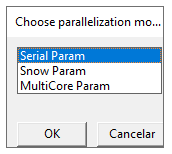
\includegraphics[width=0.25\linewidth]{01} 

}

\caption{PipMet parallelization options.}\label{fig:unnamed-chunk-4}
\end{figure}

Furthermore, the user may inform m/z and rt (retentions time) for
specific ions to be monitored throuhout the entire processing. For
example, internal standards can be monitored through the `Monitor EIC'
option.

\begin{figure}

{\centering 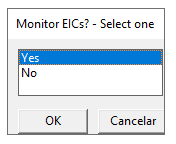
\includegraphics[width=0.25\linewidth]{02} 

}

\caption{Peak monitoring.}\label{fig:unnamed-chunk-5}
\end{figure}

As a first step, the user will be asked to point the folder where the
files to be processed are located. Once we set
\texttt{example\ =\ TRUE}, this pop-up will be supressed.

\begin{figure}

{\centering 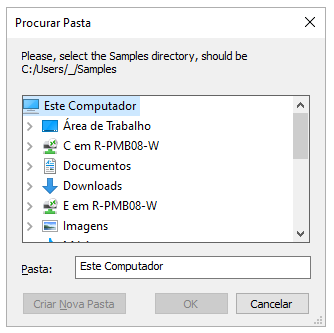
\includegraphics[width=0.4\linewidth]{1} 

}

\caption{Choose the samples folder.}\label{fig:unnamed-chunk-6}
\end{figure}

Following that, the user is asked to provide a name for the processing
project, which will be used as the name of the folder where the
processing will occur and create the output files. For the example, the
project will be named `Example'.

\begin{figure}

{\centering 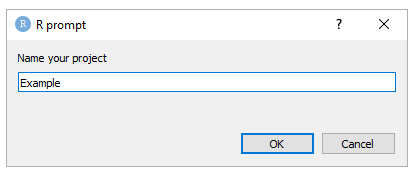
\includegraphics[width=0.4\linewidth]{2} 

}

\caption{Project folder name.}\label{fig:unnamed-chunk-7}
\end{figure}

The files extension will be asked, then, if the \texttt{example} is not
set as TRUE. The PipMet package is capable of reading `.mzML' and
`.mzXML' files through the \emph{xcms}, \emph{MSnbase} and \emph{mzR}
packages. Files with different extensions may be converted using the
\emph{Mass++} \textsuperscript{3} or \emph{Proteowizard
Softwares}\textsuperscript{4}, for example. The files provided for the
examples are .mzXML files.

\begin{figure}

{\centering 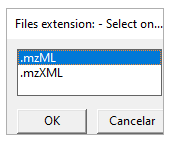
\includegraphics[width=0.25\linewidth]{3} 

}

\caption{File extensions accepted.}\label{fig:unnamed-chunk-8}
\end{figure}

The metadata file must be provided in order to proper process the
analysis files. It is a sheet .csv file containing a `sample' column for
the samples names and the `file' column with the file path to each of
the samples. Each row represent a sample. More columns can and should be
added in order to enhance grouping-demanding steps. In the set of
examples, we have two replicates of samples collected from Energycane
and two from Sugarcane, two Pool and two Blank samples. The metadata.csv
file will be as follow:

\begin{longtable}[]{@{}lll@{}}
\toprule()
sample & group & file \\
\midrule()
\endhead
20009cg02\_1 & Blank & 20009cg02\_1.mzXML \\
20009cg03\_1 & Pool & 20009cg03\_1.mzXML \\
20009cg08\_1 & Energy & 20009cg08\_1.mzXML \\
20009cg09\_1 & Energy & 20009cg09\_1.mzXML \\
20010cg02\_1 & Blank & 20010cg02\_1.mzXML \\
20010cg03\_1 & Pool & 20010cg03\_1.mzXML \\
20009cg17\_1 & Sugar & 20009cg17\_1.mzXML \\
20009cg22\_1 & Sugar & 20009cg22\_1.mzXML \\
\bottomrule()
\end{longtable}

The PipMet asks if the user already have a metadata.csv file prepared,
if the \texttt{example} is not set as TRUE. If `Yes', the user will be
asked to point the path to the metadata file. Though, if `No', a
metadat.csv file will be created with basic names for files with the
extension given in the sample\_dir so the user can fill it.

\begin{figure}

{\centering 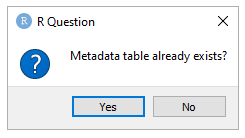
\includegraphics[width=0.35\linewidth]{4} 

}

\caption{Metadata table.}\label{fig:unnamed-chunk-10}
\end{figure}

Here, the user may create different categories to describe the samples
with simples name as column names. It is important to make sure there is
no other filled columns or rows except those containing the samples. For
that, select the empty columns and rows and delete its content before
saving. If there is the content, the software will alert the user to
delete and reupload the metadata file.

\begin{figure}

{\centering 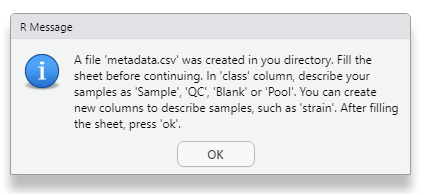
\includegraphics[width=0.5\linewidth]{5} 

}

\caption{Metadata information.}\label{fig:unnamed-chunk-11}
\end{figure}

When the files are properly read, a `Visualization\_results' folder will
be created in your project folder the software saves generated pictures
for the user to evaluate the quality of the initial data, such as total
ion count and base peak chromatograms and heatmaps

\begin{figure}

{\centering 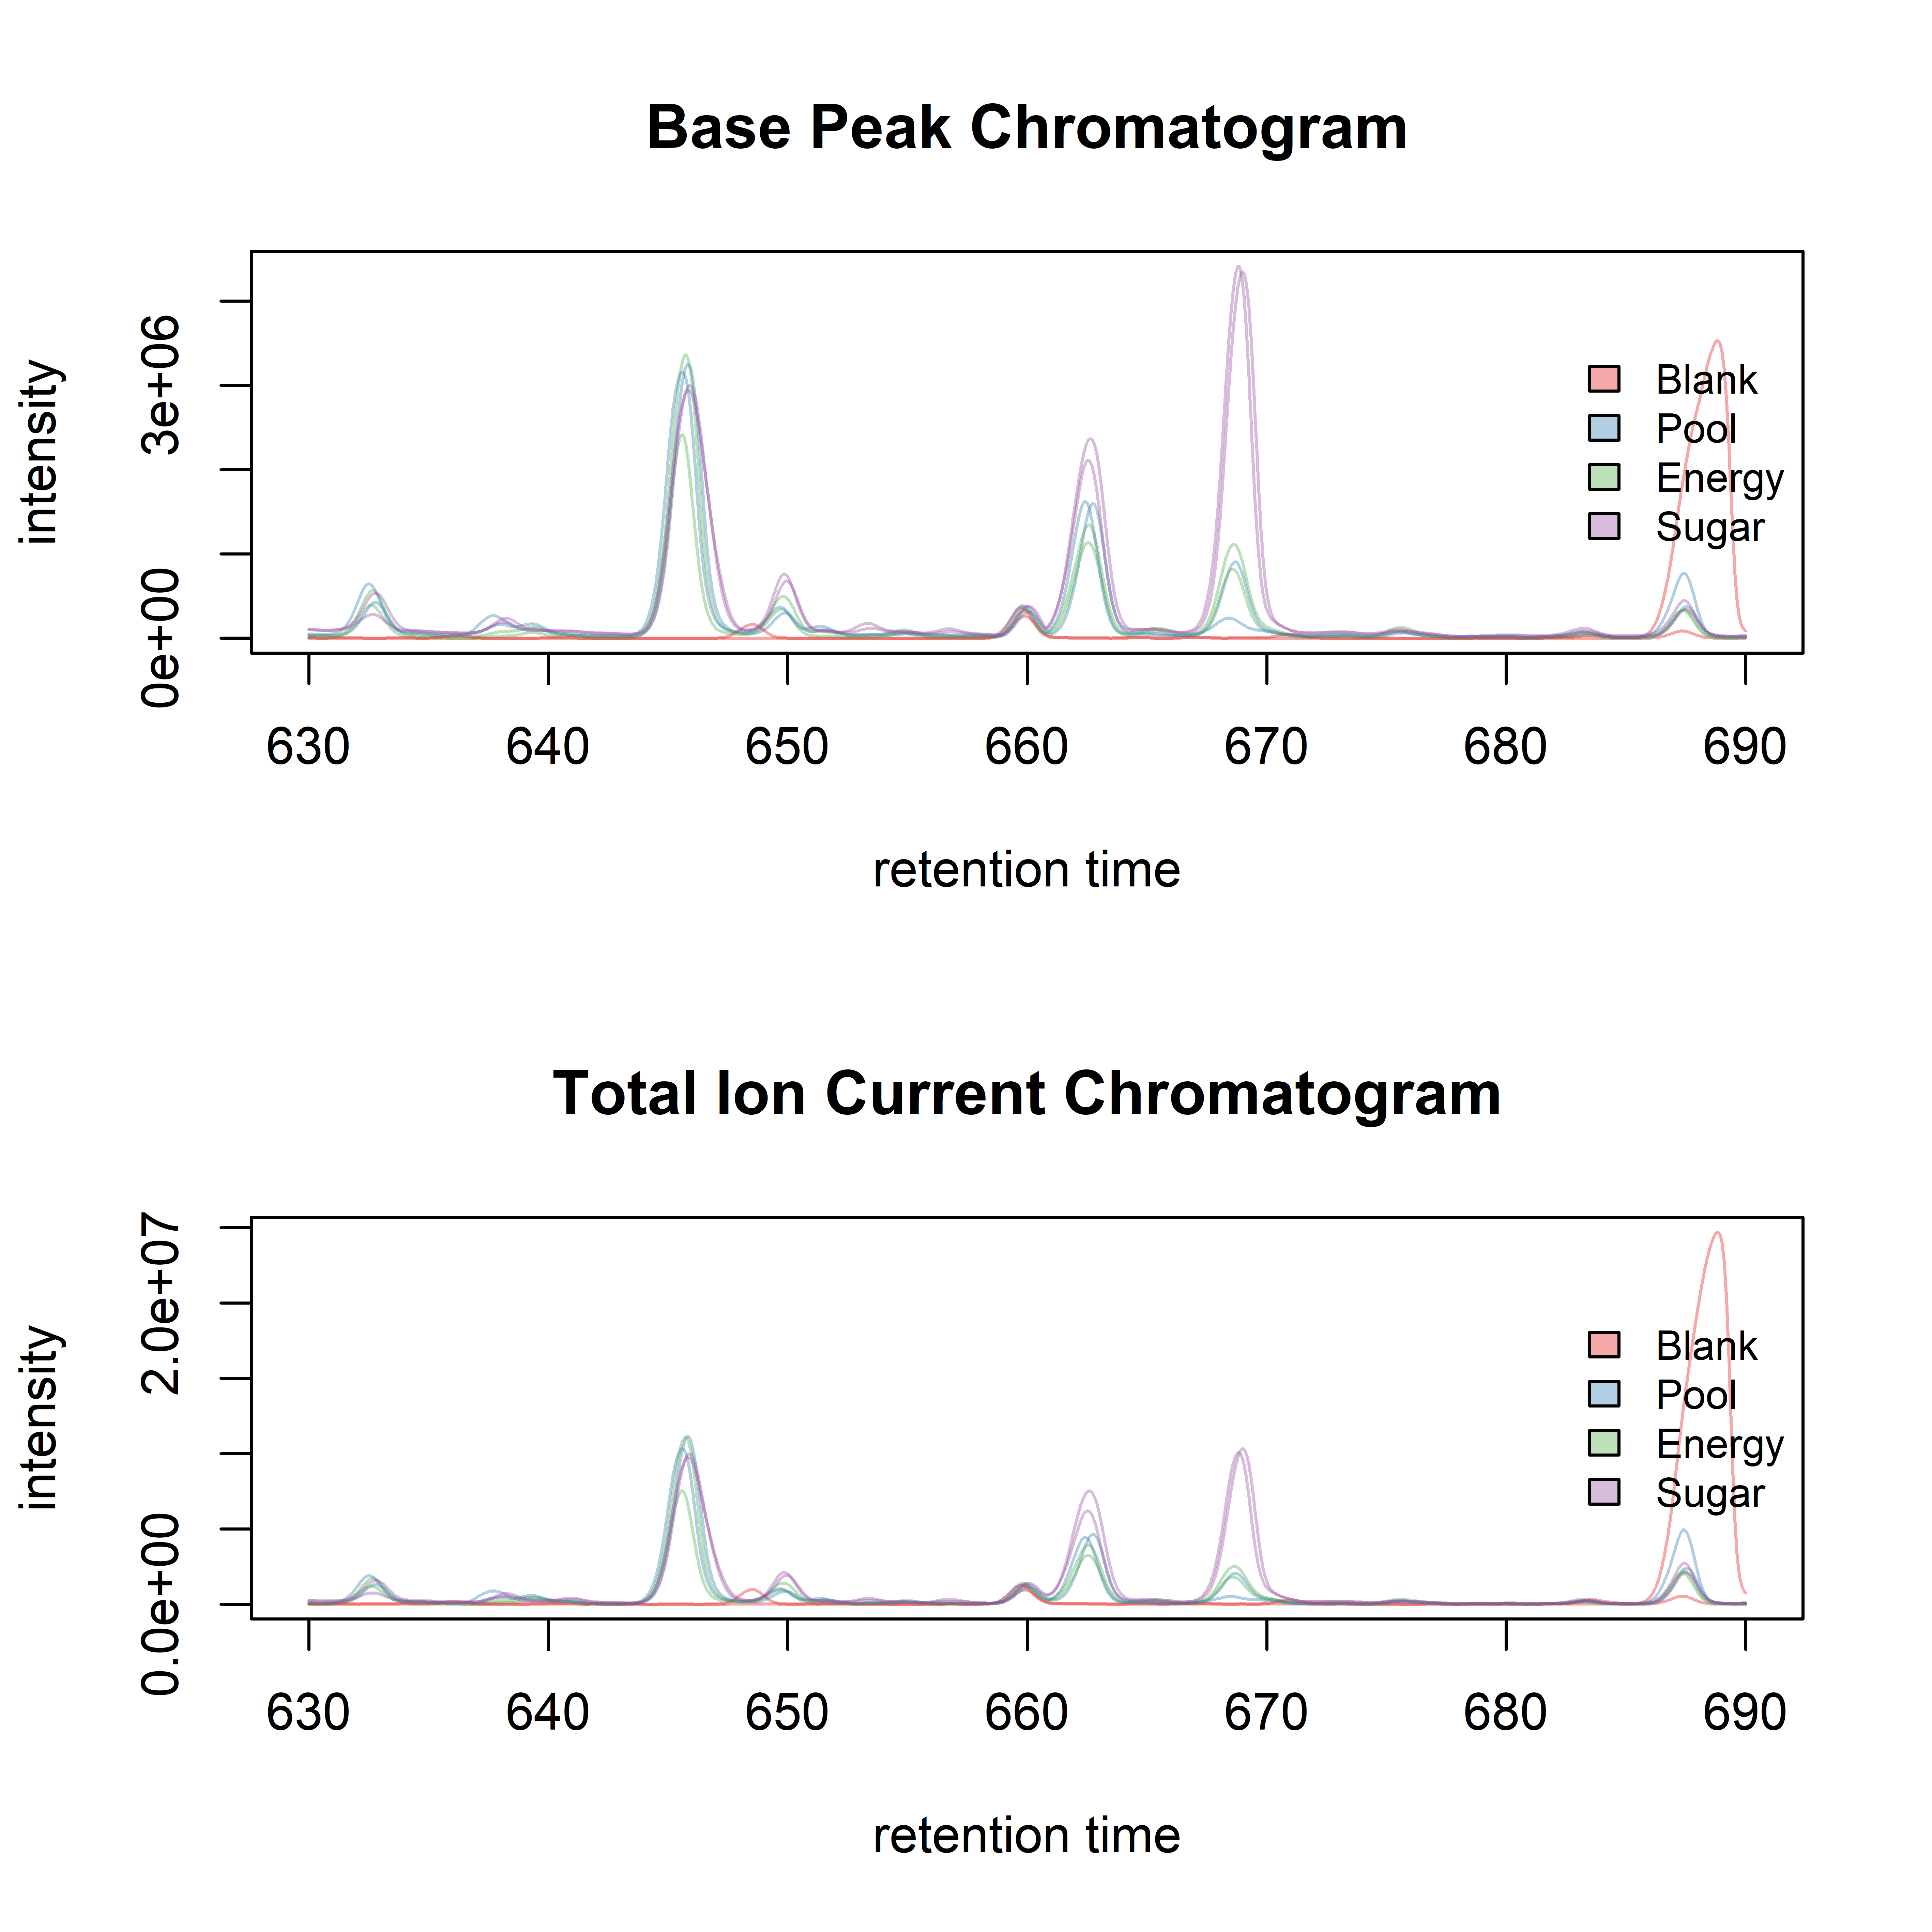
\includegraphics[width=0.8\linewidth]{group_chromatograms} 

}

\caption{Chromatograms of the samples.}\label{fig:unnamed-chunk-12}
\end{figure}
\begin{figure}

{\centering 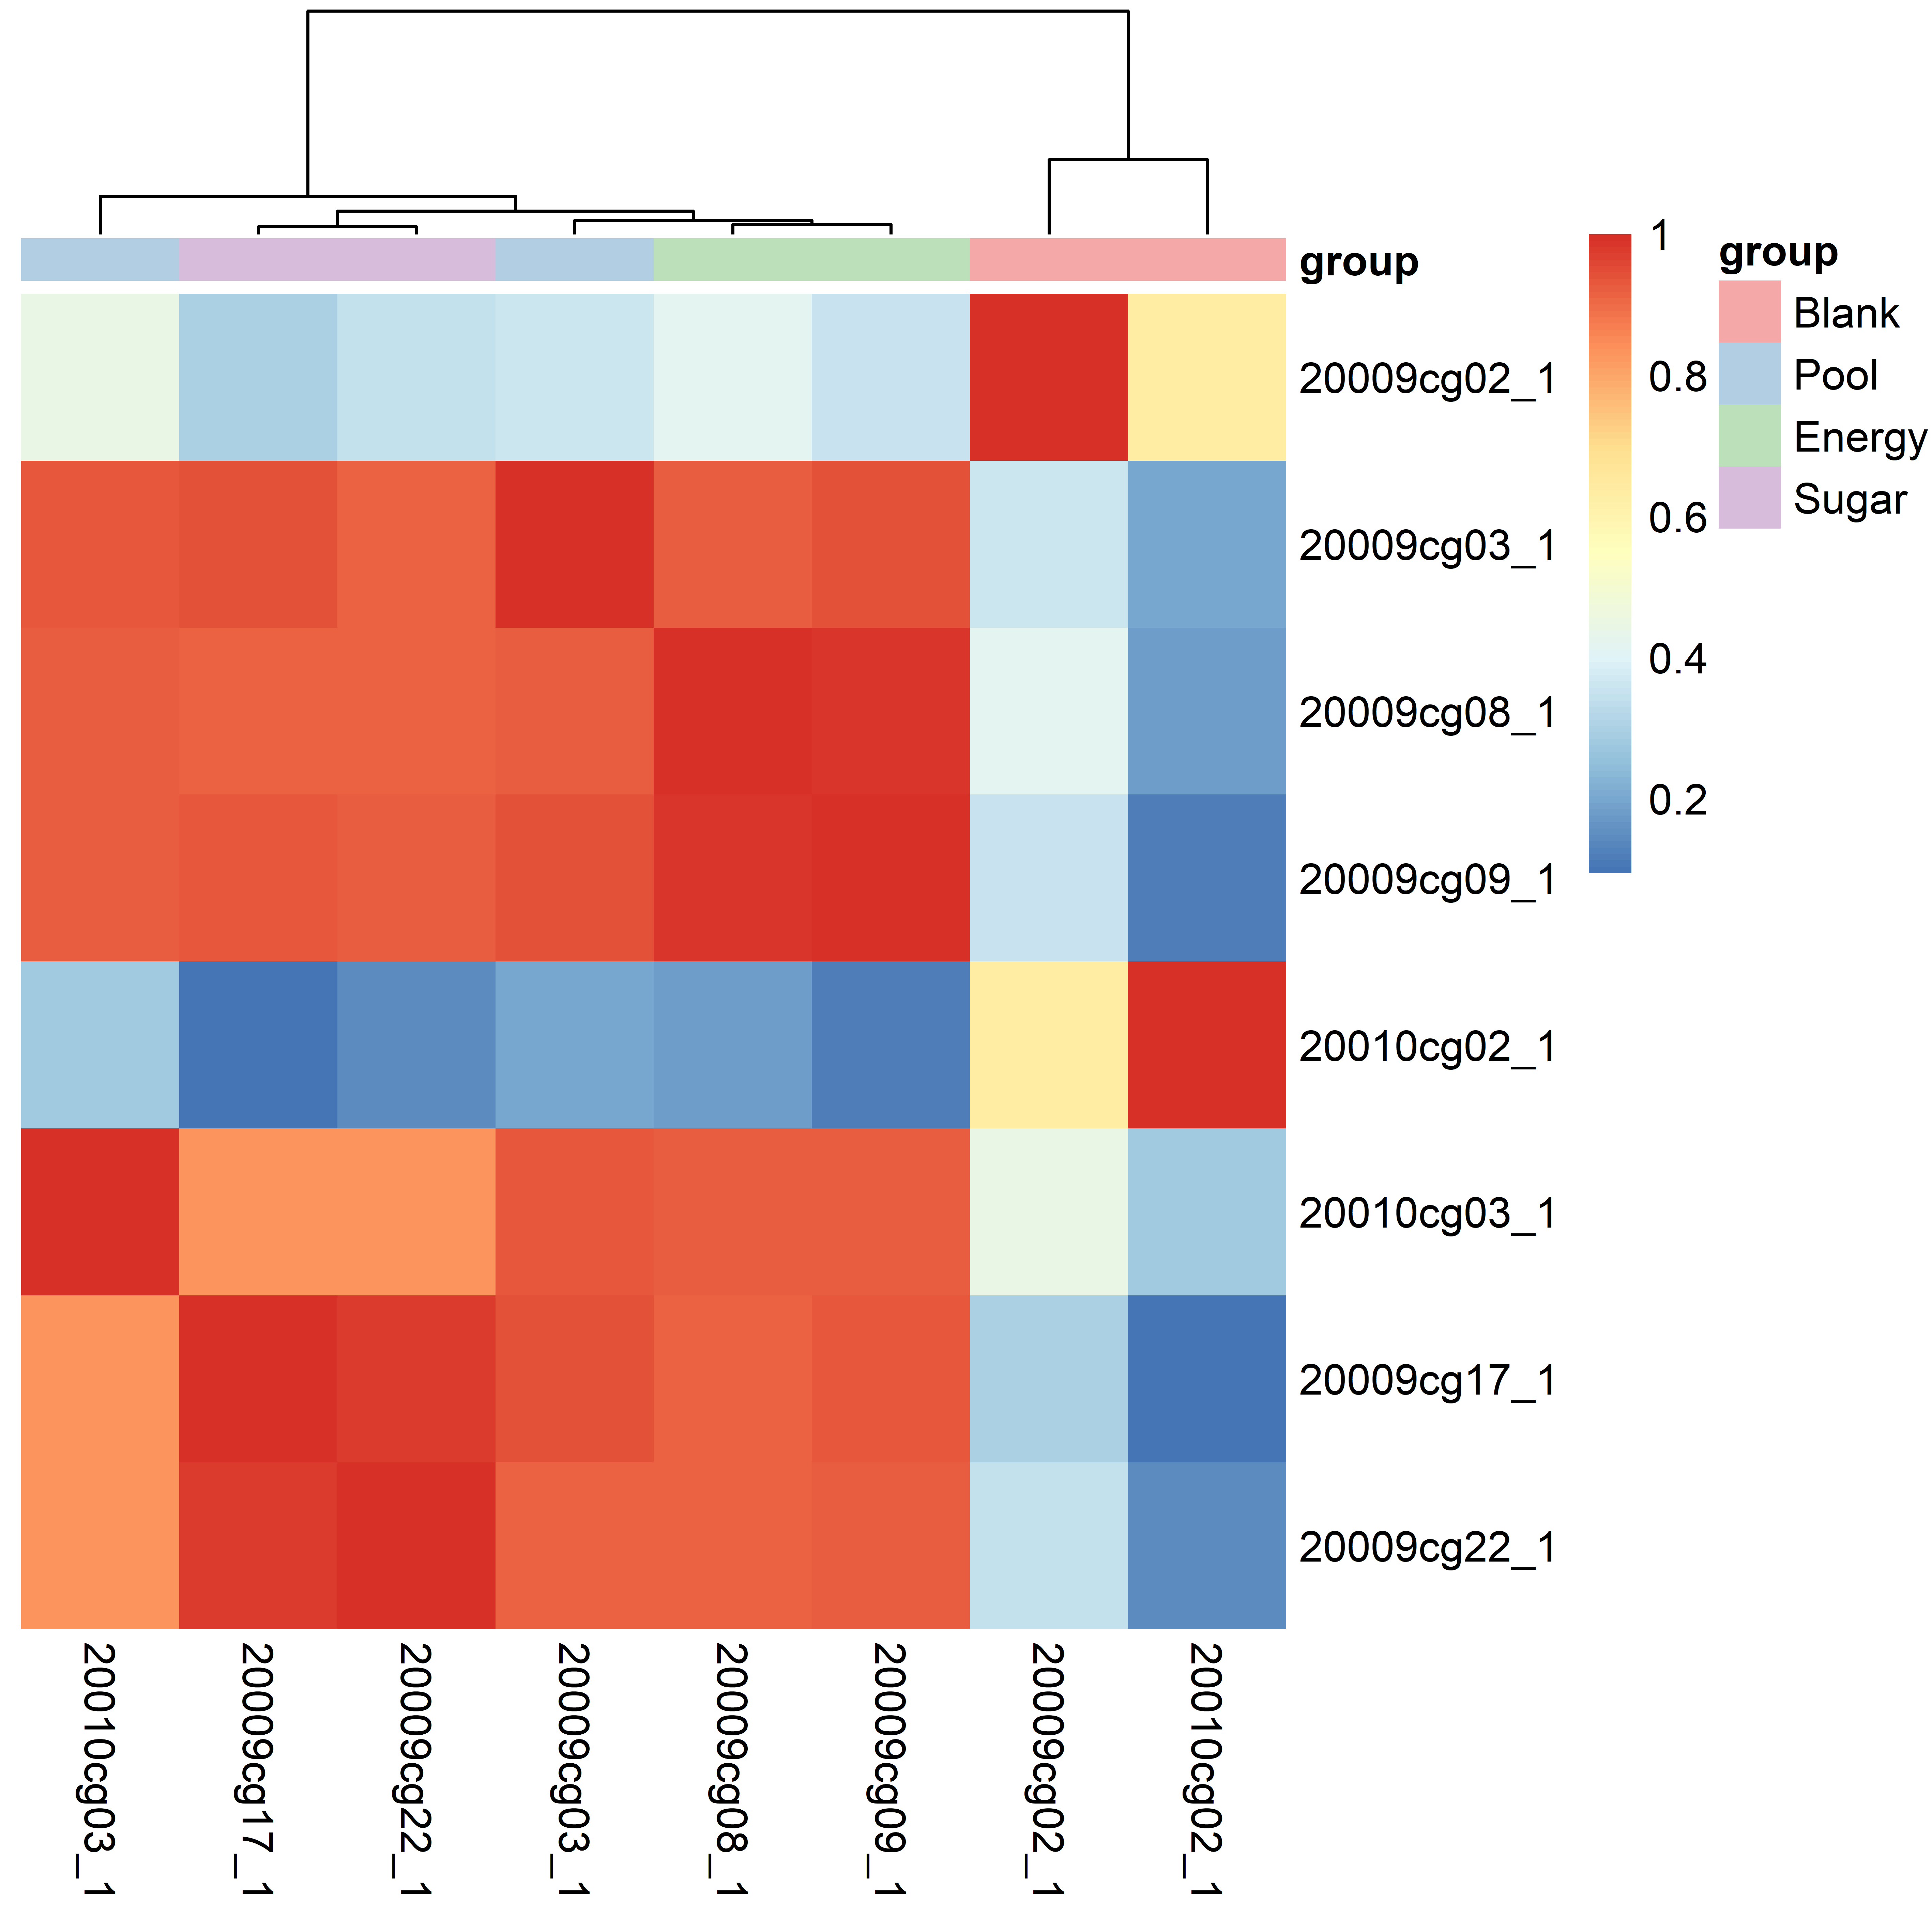
\includegraphics[width=0.8\linewidth]{group_sample__cluster} 

}

\caption{Cluster of the samples.}\label{fig:unnamed-chunk-13}
\end{figure}

\hypertarget{preprocessing}{%
\subsection{Preprocessing}\label{preprocessing}}

The first step in the preprocessing phase is the selection of peaks
among noise, done with the MatchedFilter algorythm from xcms. Therefore,
the true peaks will be picked as the one that can pass gaussian filters.
There is also de possibility of applying a filter to selec only peaks
above a certain intensity threshold.In the present example, we will be
using a 150 intensity threshold for final spectra quality improvement.

\begin{figure}

{\centering 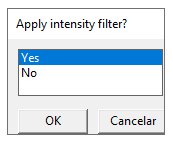
\includegraphics[width=0.25\linewidth]{6} 

}

\caption{Intensity filter.}\label{fig:unnamed-chunk-14}
\end{figure}
\begin{figure}

{\centering 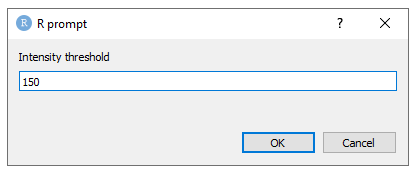
\includegraphics[width=0.4\linewidth]{7} 

}

\caption{Intensity threshold.}\label{fig:unnamed-chunk-15}
\end{figure}

Afterwards, a retention time correction and features grouping algorythms
will be applied and the user may also be asked to provide one category
from the metadata to lead the grouping step if there is more than one.
As a final step to the pre-processing step regarding to select viable
peaks, the raw data is used to fill peaks that seems to be missing.

As the previous step, the processing step generates multiple images so
that the user can evaluate the performance of the algorithms
implemented, such as chromatograms comparing the pre- and
post-processing steps, a boxplot of the samples intensities and a
distribution of peaks detected along the retention time for each of the
samples.

\begin{figure}

{\centering 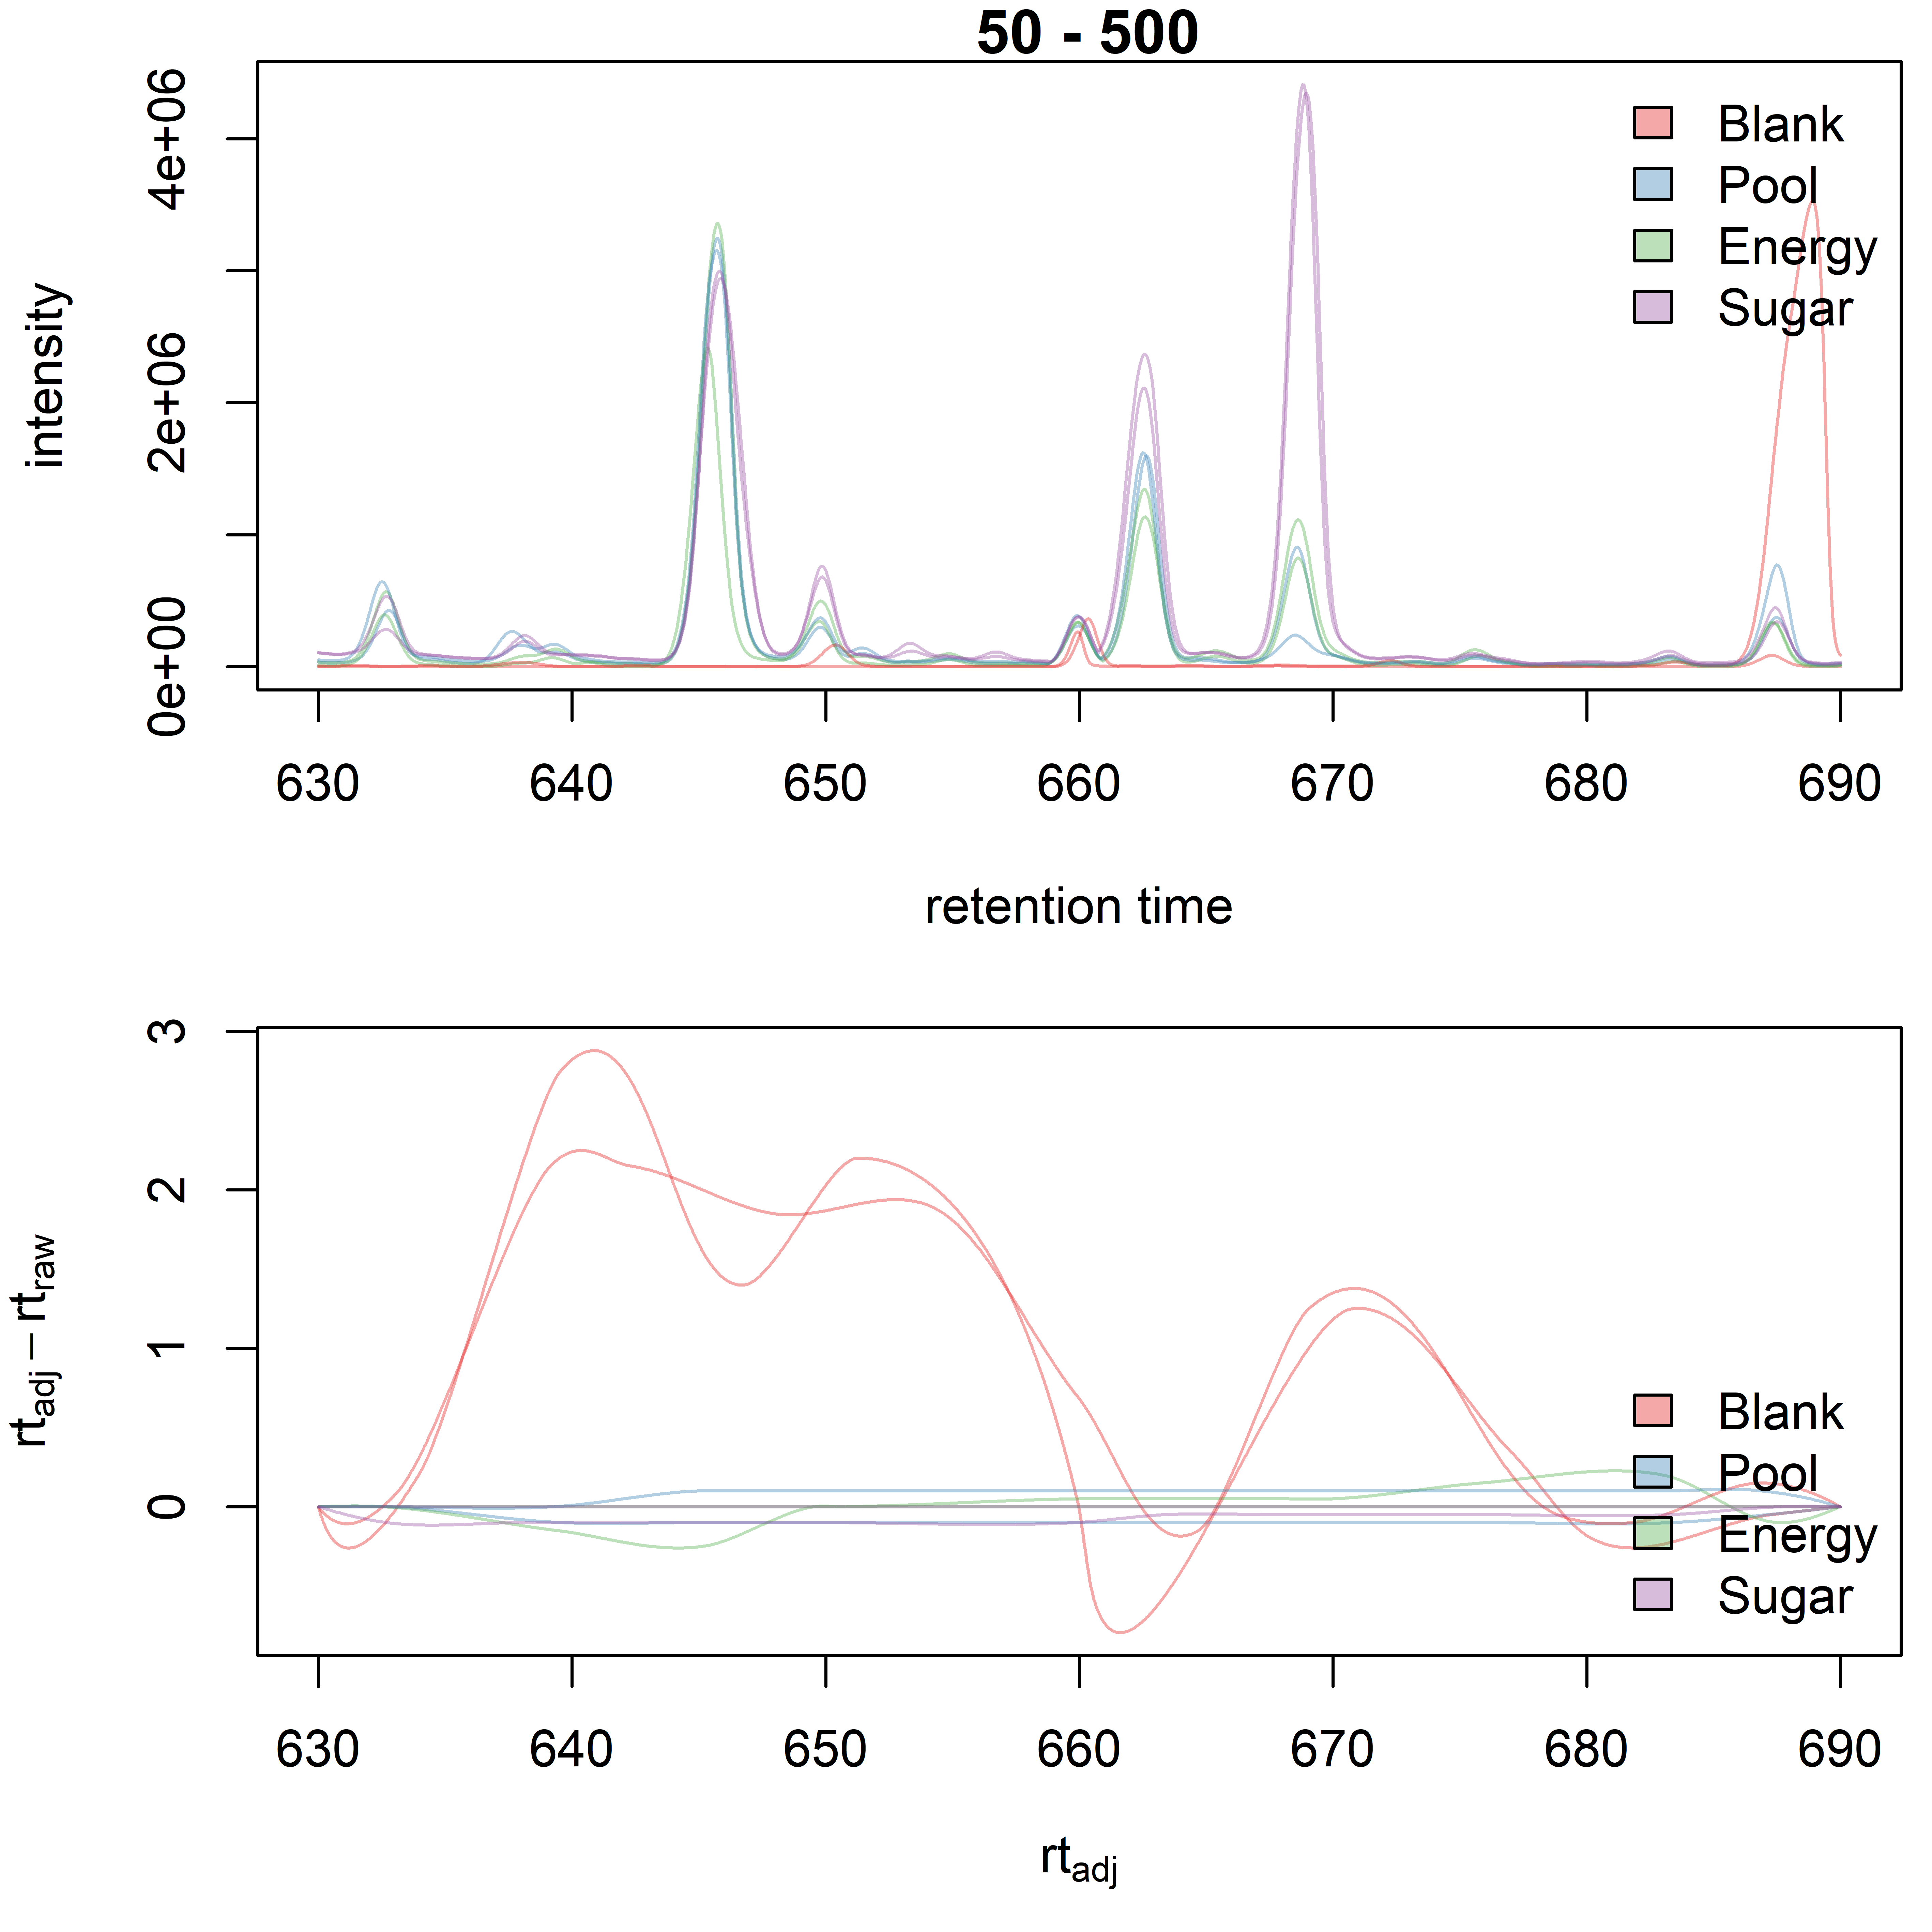
\includegraphics[width=0.8\linewidth]{group_postprocessedChromatogram} 

}

\caption{Chromatograms postprocessing.}\label{fig:unnamed-chunk-16}
\end{figure}
\begin{figure}

{\centering 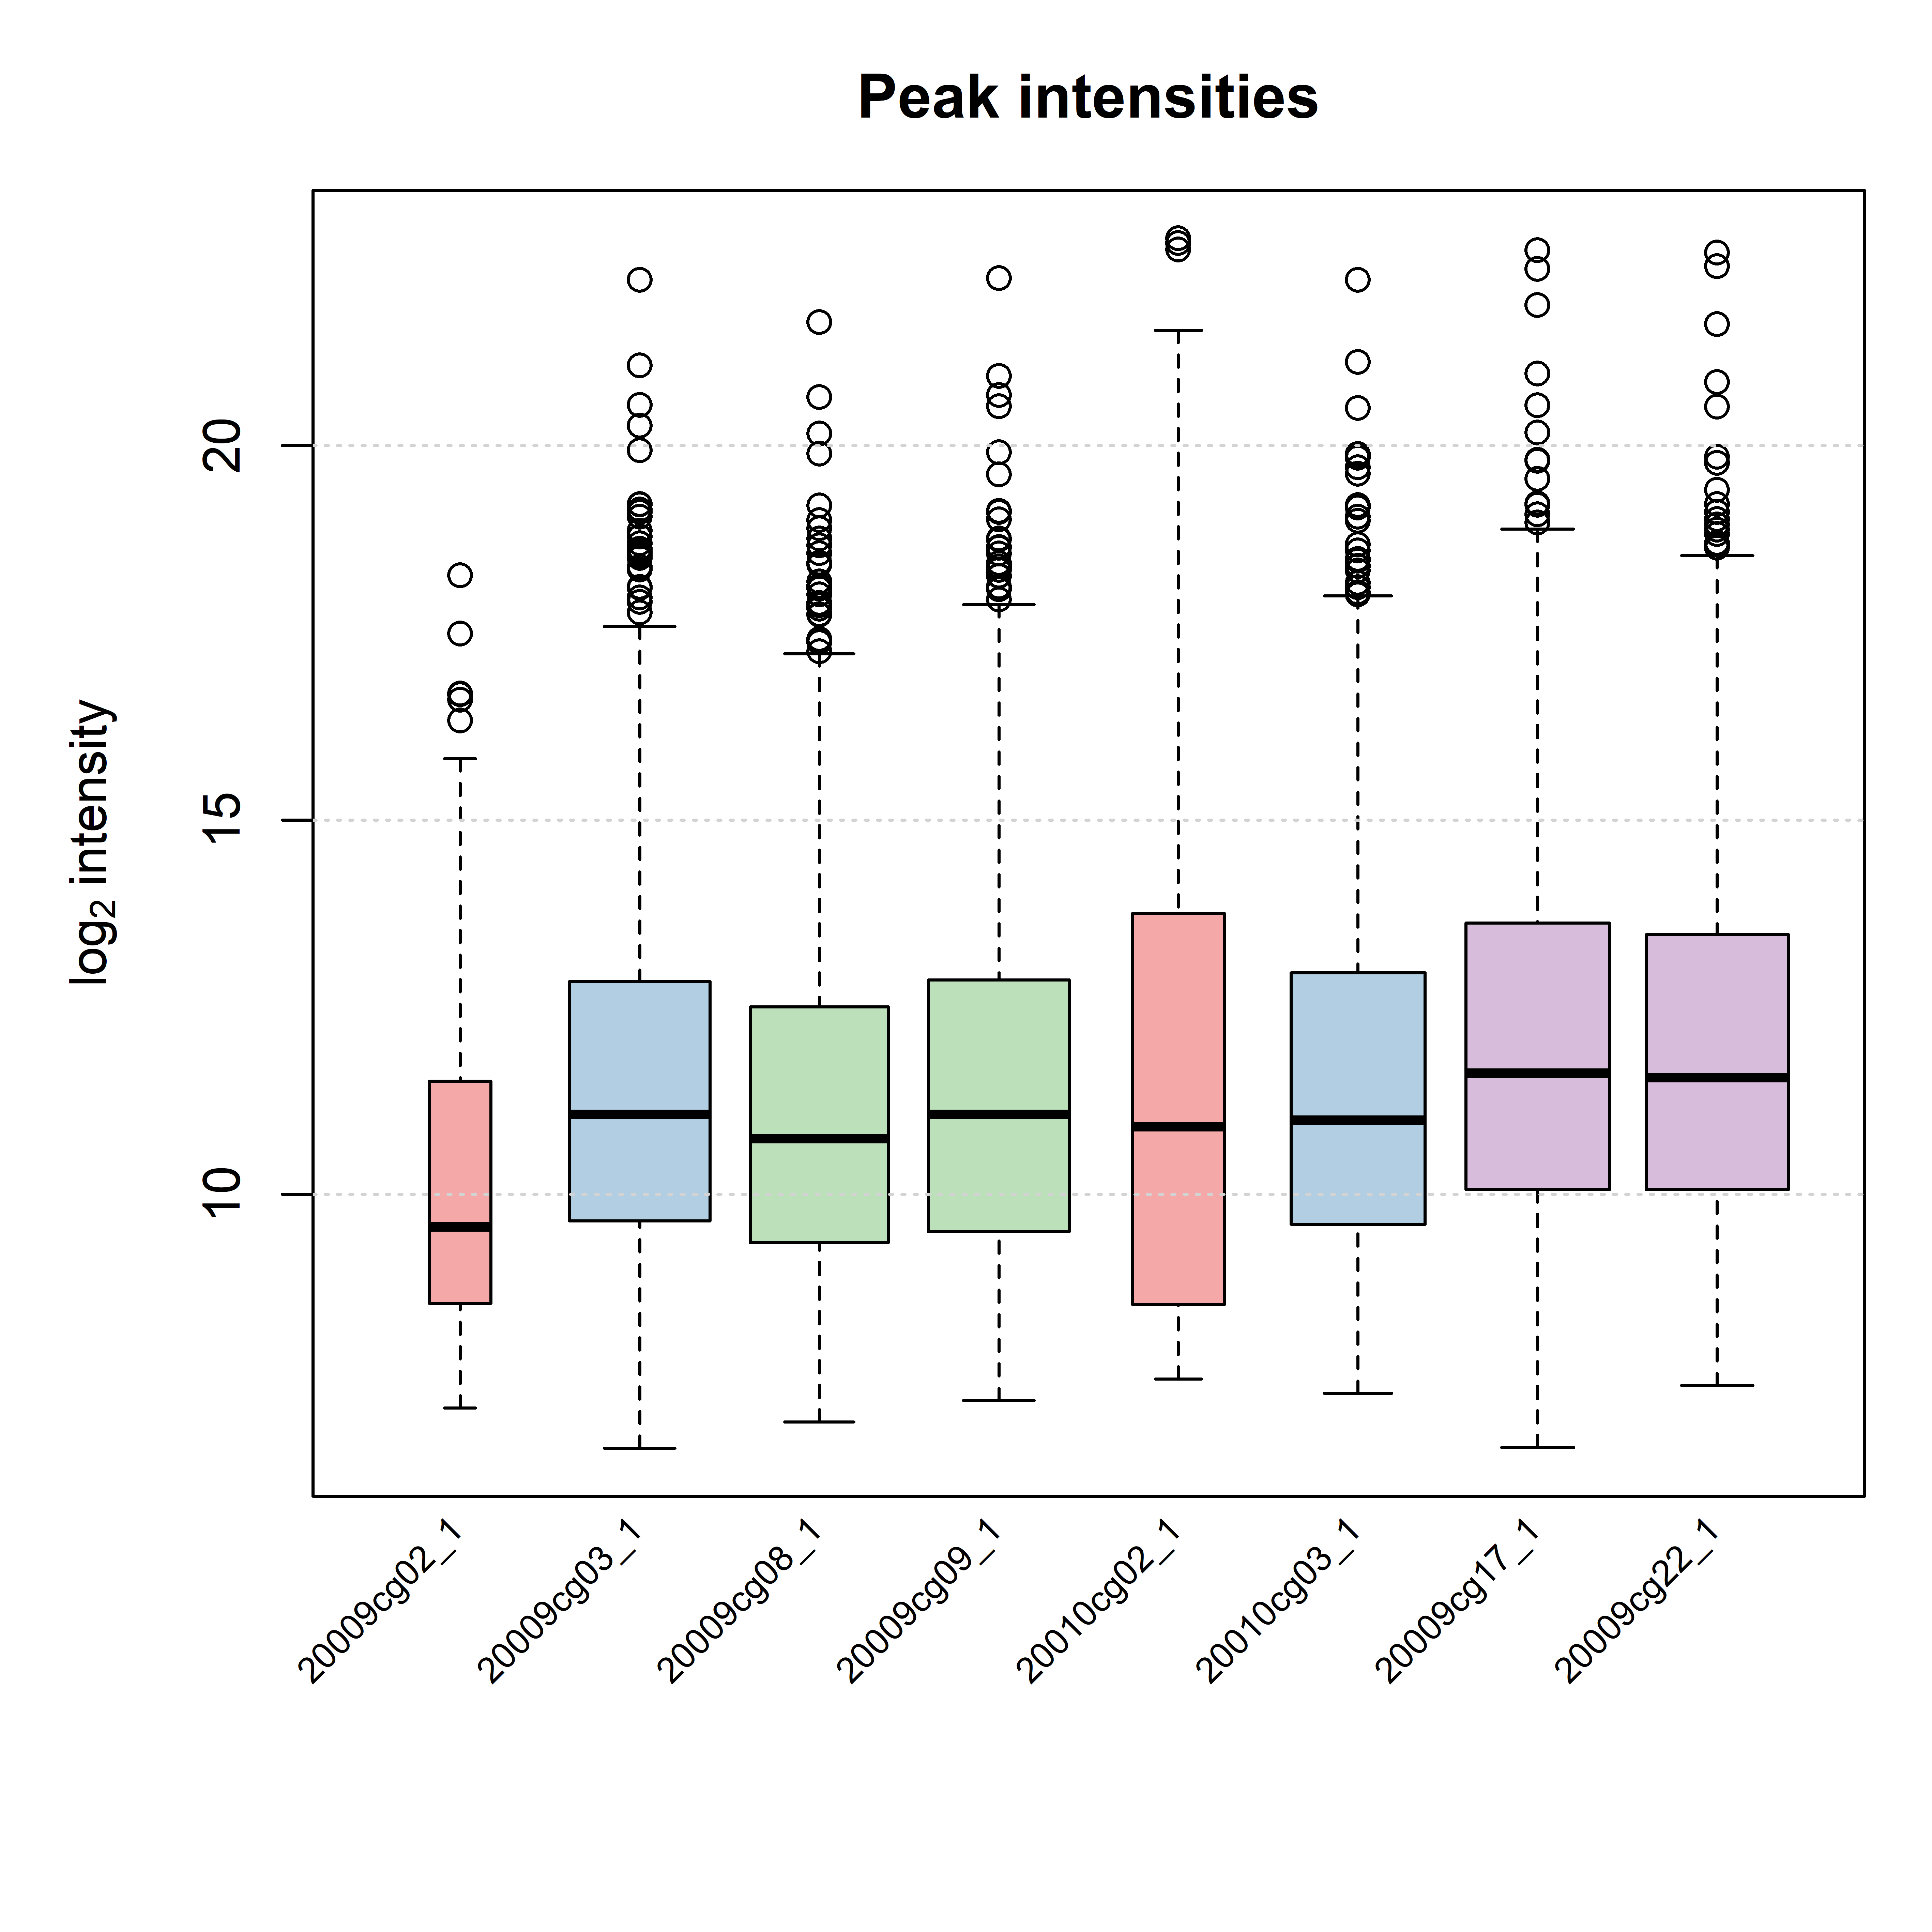
\includegraphics[width=0.8\linewidth]{group_boxplotLog2Postprocessed} 

}

\caption{Boxplot of intensities postprocessing.}\label{fig:unnamed-chunk-17}
\end{figure}
\begin{figure}

{\centering 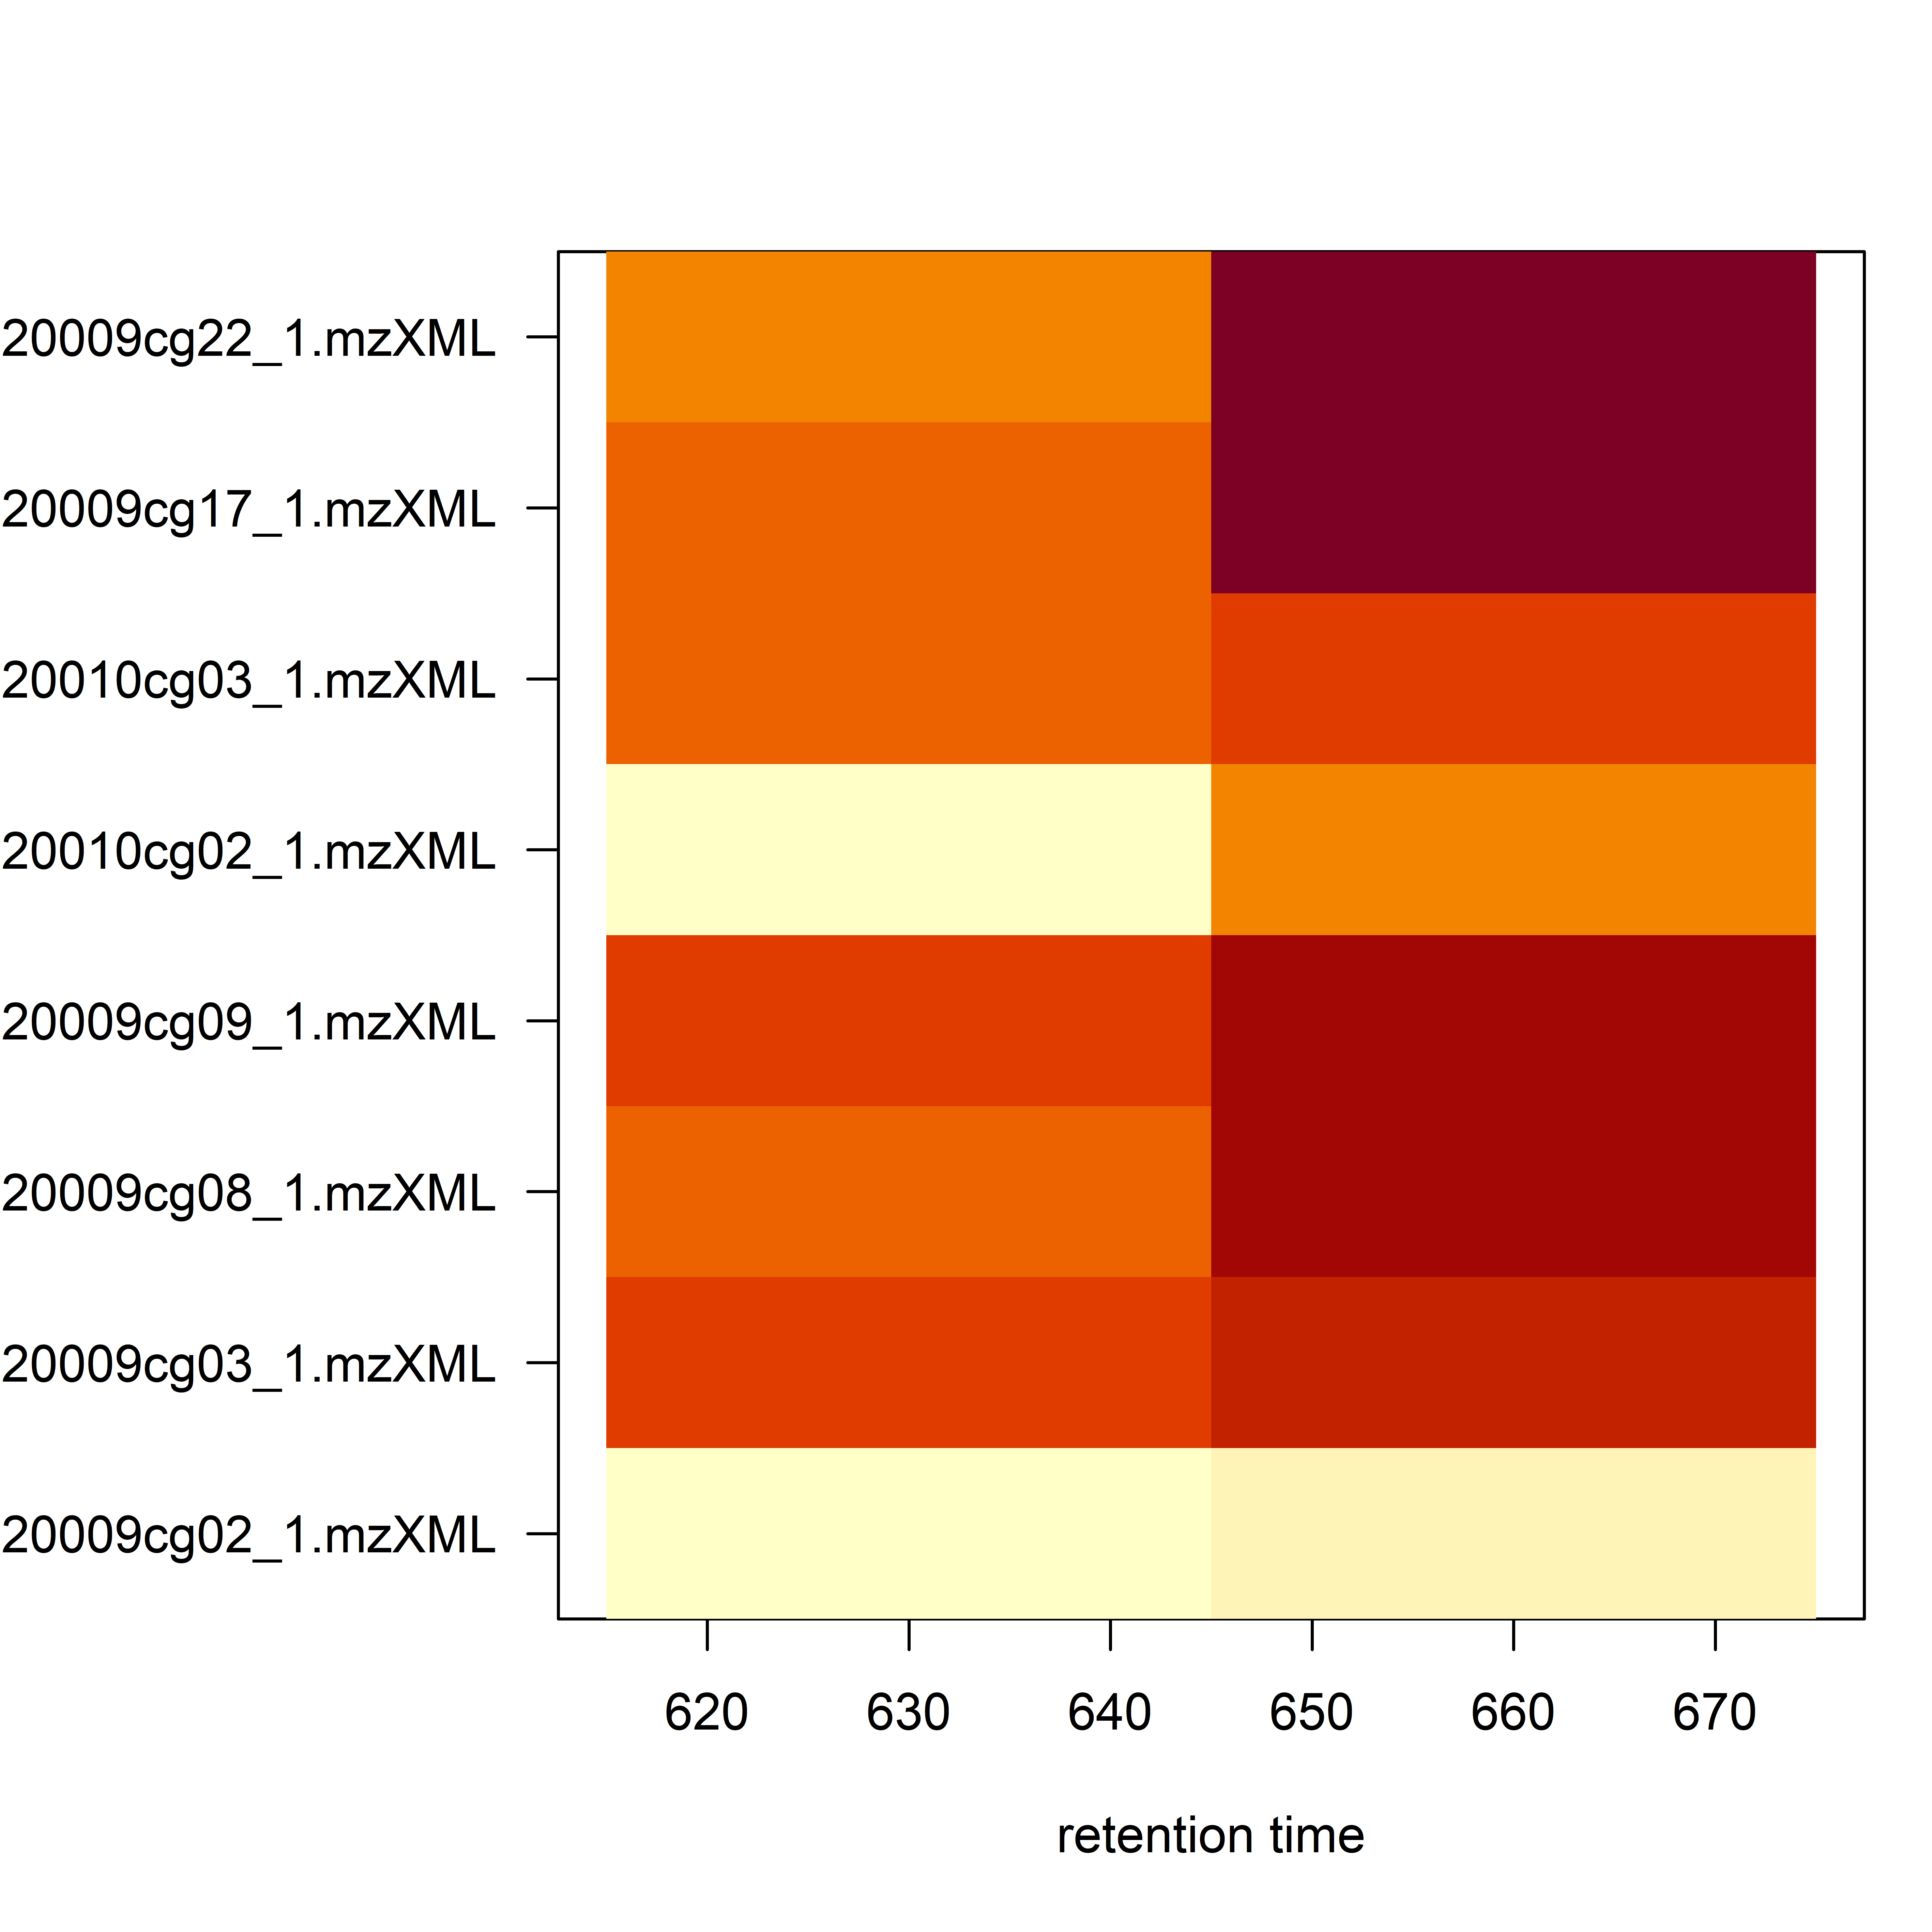
\includegraphics[width=0.8\linewidth]{plotChromPeakImage} 

}

\caption{Intensity of detected peaks in postprocessed data.}\label{fig:unnamed-chunk-18}
\end{figure}

\hypertarget{identification}{%
\subsection{Identification}\label{identification}}

\hypertarget{spectra-definition}{%
\subsubsection{Spectra definition}\label{spectra-definition}}

The peaks selected are furthered grouped into spectra using retention
time information and correlation information among the peaks. The user
will be asked the data acquisition mode (positive and negative), column
setup (polar and non-polar), temperatura program (isothermal, ramp,
custom). For the example, select the following: `positive', `non-polar'
and `ramp'.

\hypertarget{annotation}{%
\subsubsection{Annotation}\label{annotation}}

When the spectra are finalized, the PipMet software will create a .msp
file and a pre\_anno.csv file. The first is to be uploaded in the NIST
MS Search Software \textsuperscript{2} for the spectra search in the
available databases. Also, it is possible to generate a .pdf file with
EIC of the 6 most intense ions of each of spectrum.

\begin{figure}

{\centering 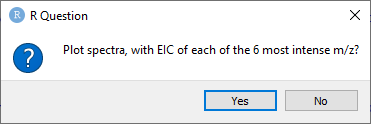
\includegraphics[width=0.5\linewidth]{03} 

}

\caption{Extracted ion chromatogram.}\label{fig:unnamed-chunk-19}
\end{figure}

The user must identify each of the spectrum and write the name of the
compound identified in the pre\_anno.csv sheet, using the id of the
spectrum, present in the .msp file and the table in pre\_anno.
Non-indentified spectra may remaining unnanotated. When finished, the
user must save the pre\_anno.csv file and click `Ok' in the pop-up.

\begin{figure}

{\centering 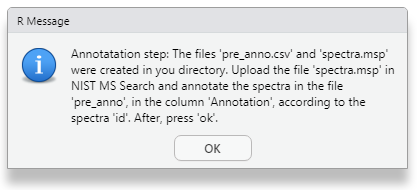
\includegraphics[width=0.5\linewidth]{9} 

}

\caption{Spectra annotation.}\label{fig:unnamed-chunk-20}
\end{figure}

For the 30 spectra generated, the pre\_anno.csv with the annotation
information is as follow:

\begin{longtable}[]{@{}rlrl@{}}
\toprule()
id & mz & rt & annotation \\
\midrule()
\endhead
1 & NA & 669.1000 & \\
2 & NA & 667.1472 & \\
3 & NA & 687.3255 & Palmitic acid \\
4 & NA & 645.7250 & Inositol \\
5 & NA & 662.4250 & \\
6 & NA & 650.3799 & Tyrosine \\
7 & NA & 632.7000 & Allantoin \\
8 & NA & 660.1515 & FAME C16 \\
9 & NA & 637.4276 & \\
10 & NA & 661.4000 & \\
12 & NA & 646.9499 & \\
13 & NA & 633.7106 & \\
14 & NA & 638.5364 & \\
15 & NA & 640.3500 & \\
16 & NA & 664.7471 & \\
18 & NA & 688.5554 & \\
19 & NA & 637.6735 & \\
21 & NA & 654.7856 & \\
23 & NA & 675.7625 & \\
24 & NA & 669.8623 & \\
25 & NA & 683.1997 & \\
27 & NA & 653.3966 & \\
28 & NA & 656.5103 & \\
29 & NA & 652.1000 & \\
33 & NA & 676.7077 & p-Coummaric acid \\
38 & NA & 680.5215 & \\
82 & NA & 639.2010 & \\
115 & NA & 683.1962 & \\
138 & NA & 679.7216 & \\
\bottomrule()
\end{longtable}

The annotation may vary due to different available libraries in the NIST
MS Search software. For improving the identification, the retention
index can also be used, if a RI.csv file is provided, containing a `rt'
and `RI' column. Once the example files are of a slim range of retention
time, we will not add any retention index.

\begin{figure}

{\centering 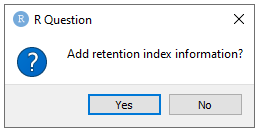
\includegraphics[width=0.5\linewidth]{12} 

}

\caption{Retention index.}\label{fig:unnamed-chunk-22}
\end{figure}

At the end of this substep, some pictures are plotted, such as
hierarchycal clustering and a heatmaps based on the similarity of the
samples. For more information, check the CluMSID R package.

\begin{figure}

{\centering 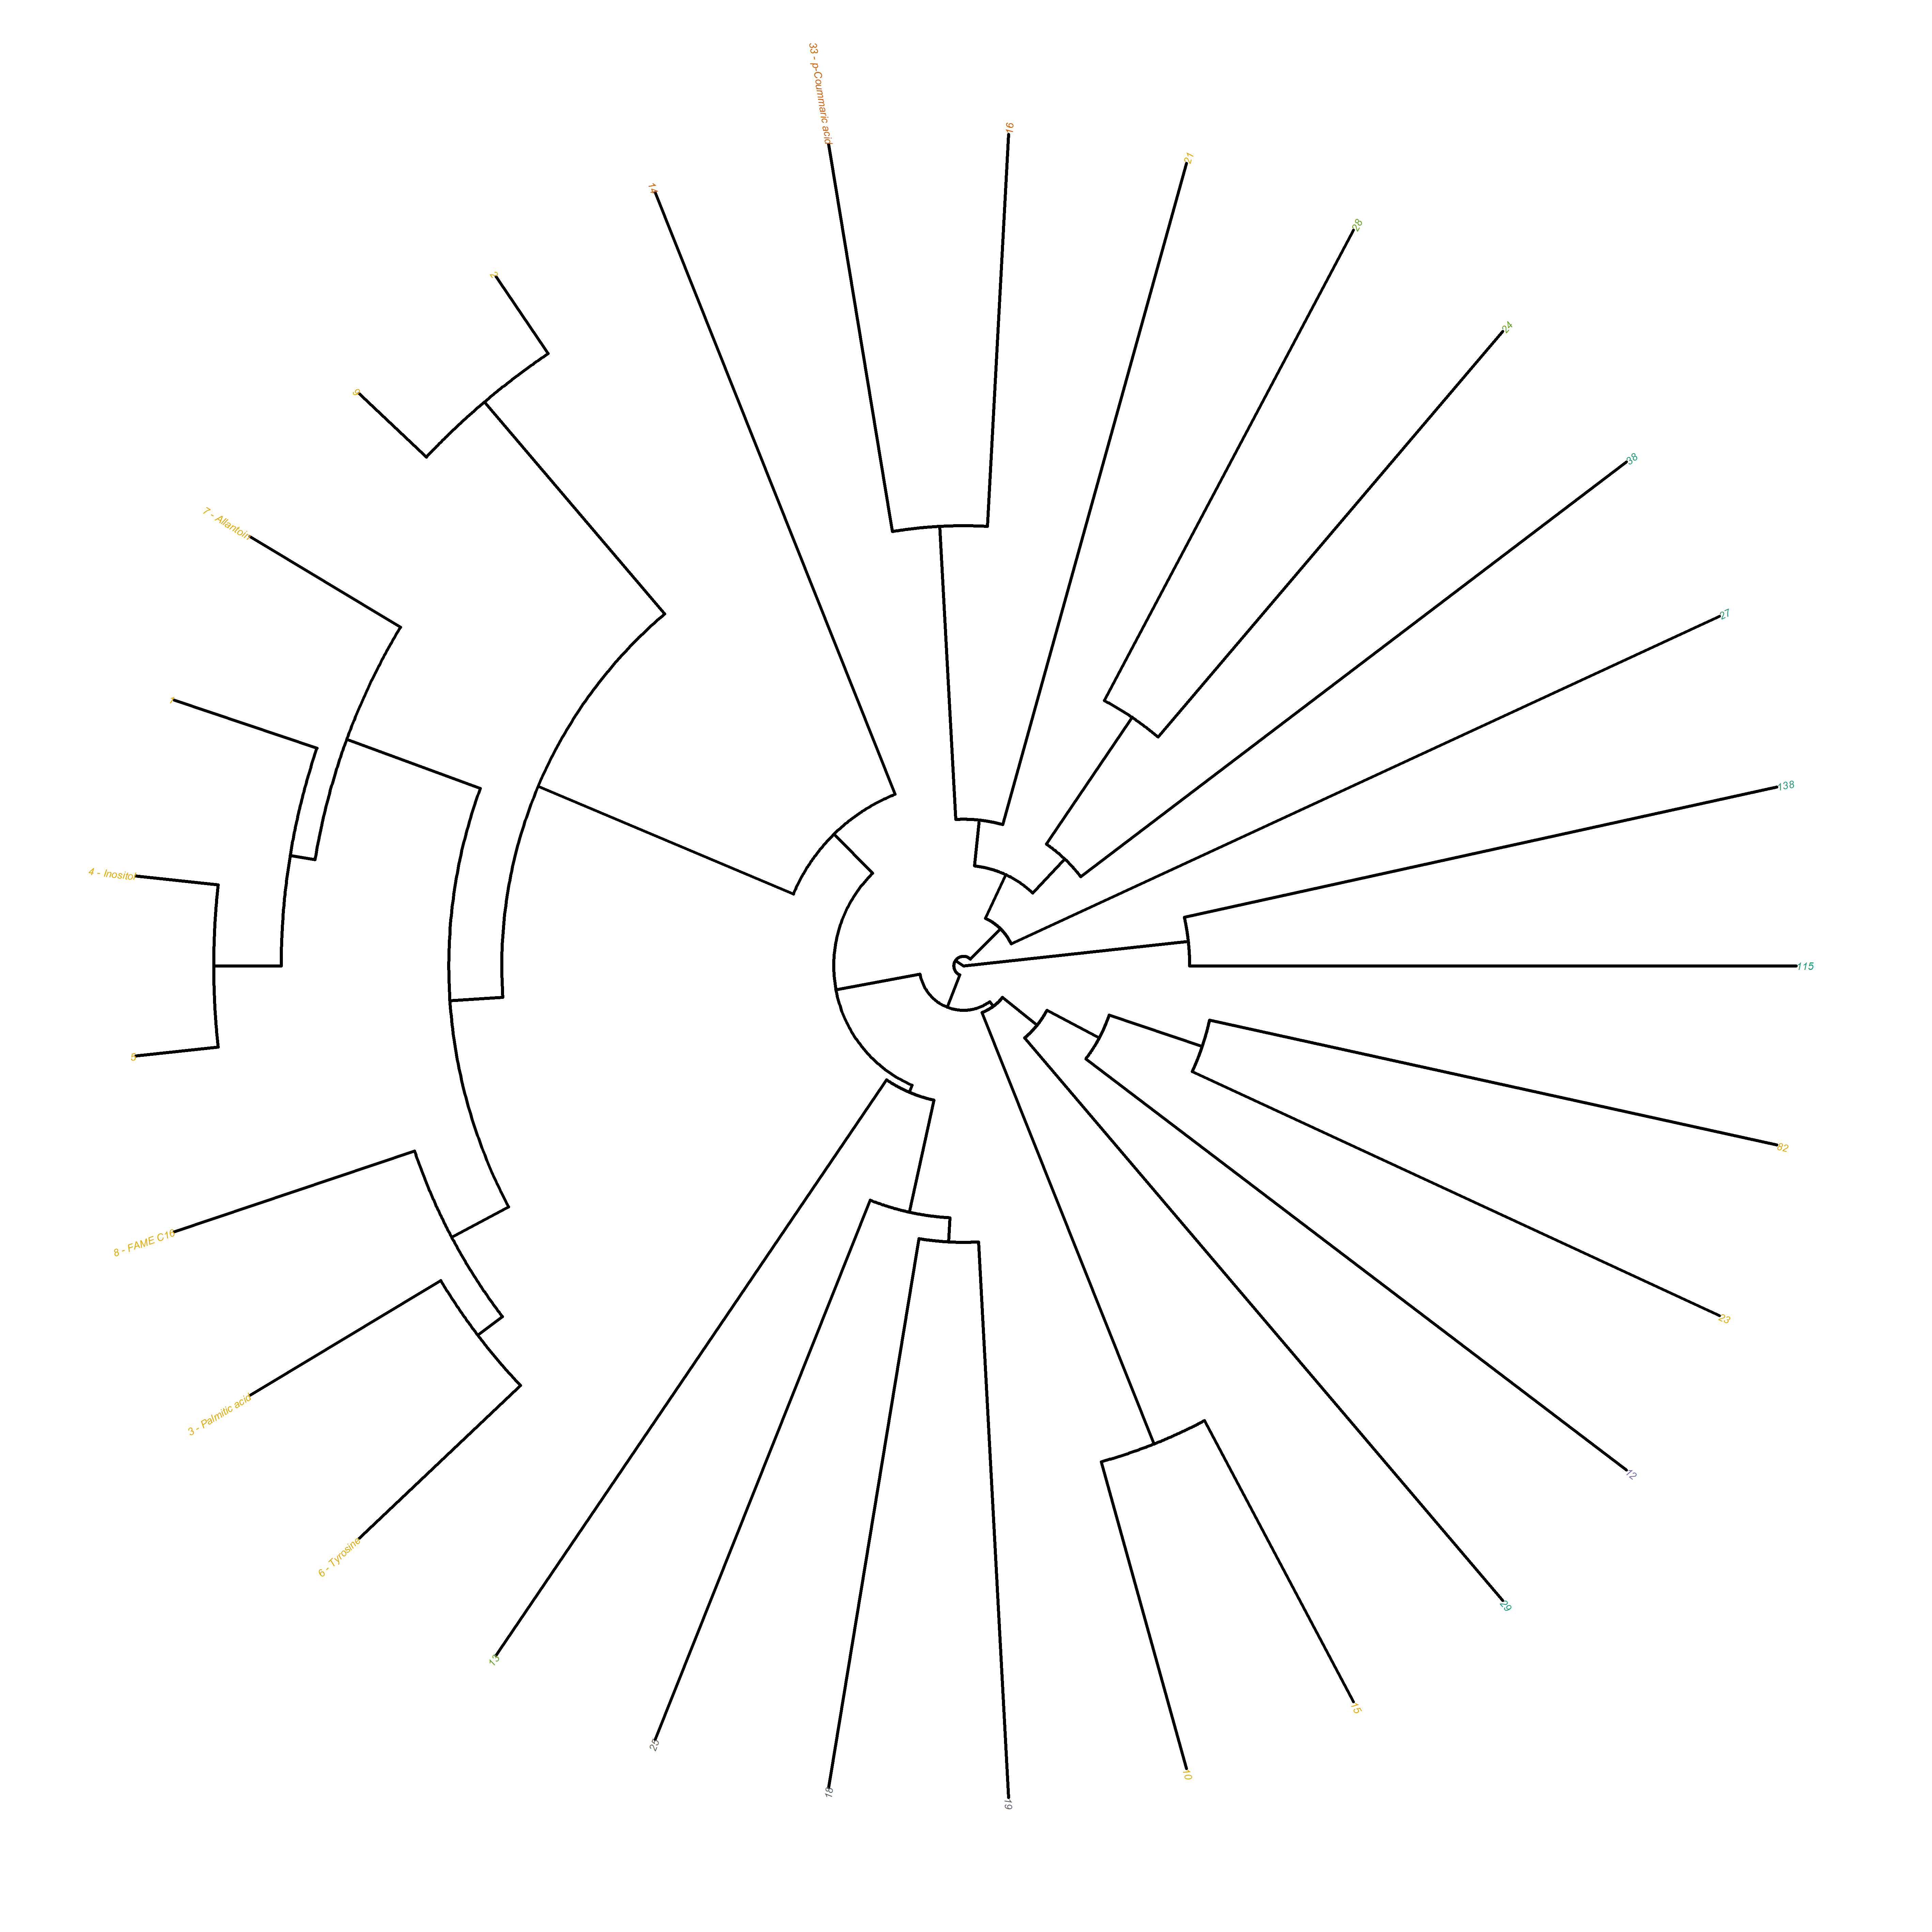
\includegraphics[width=1\linewidth]{hierarchy_plot} 

}

\caption{Hierarchycal plot.}\label{fig:unnamed-chunk-23}
\end{figure}
\begin{figure}

{\centering 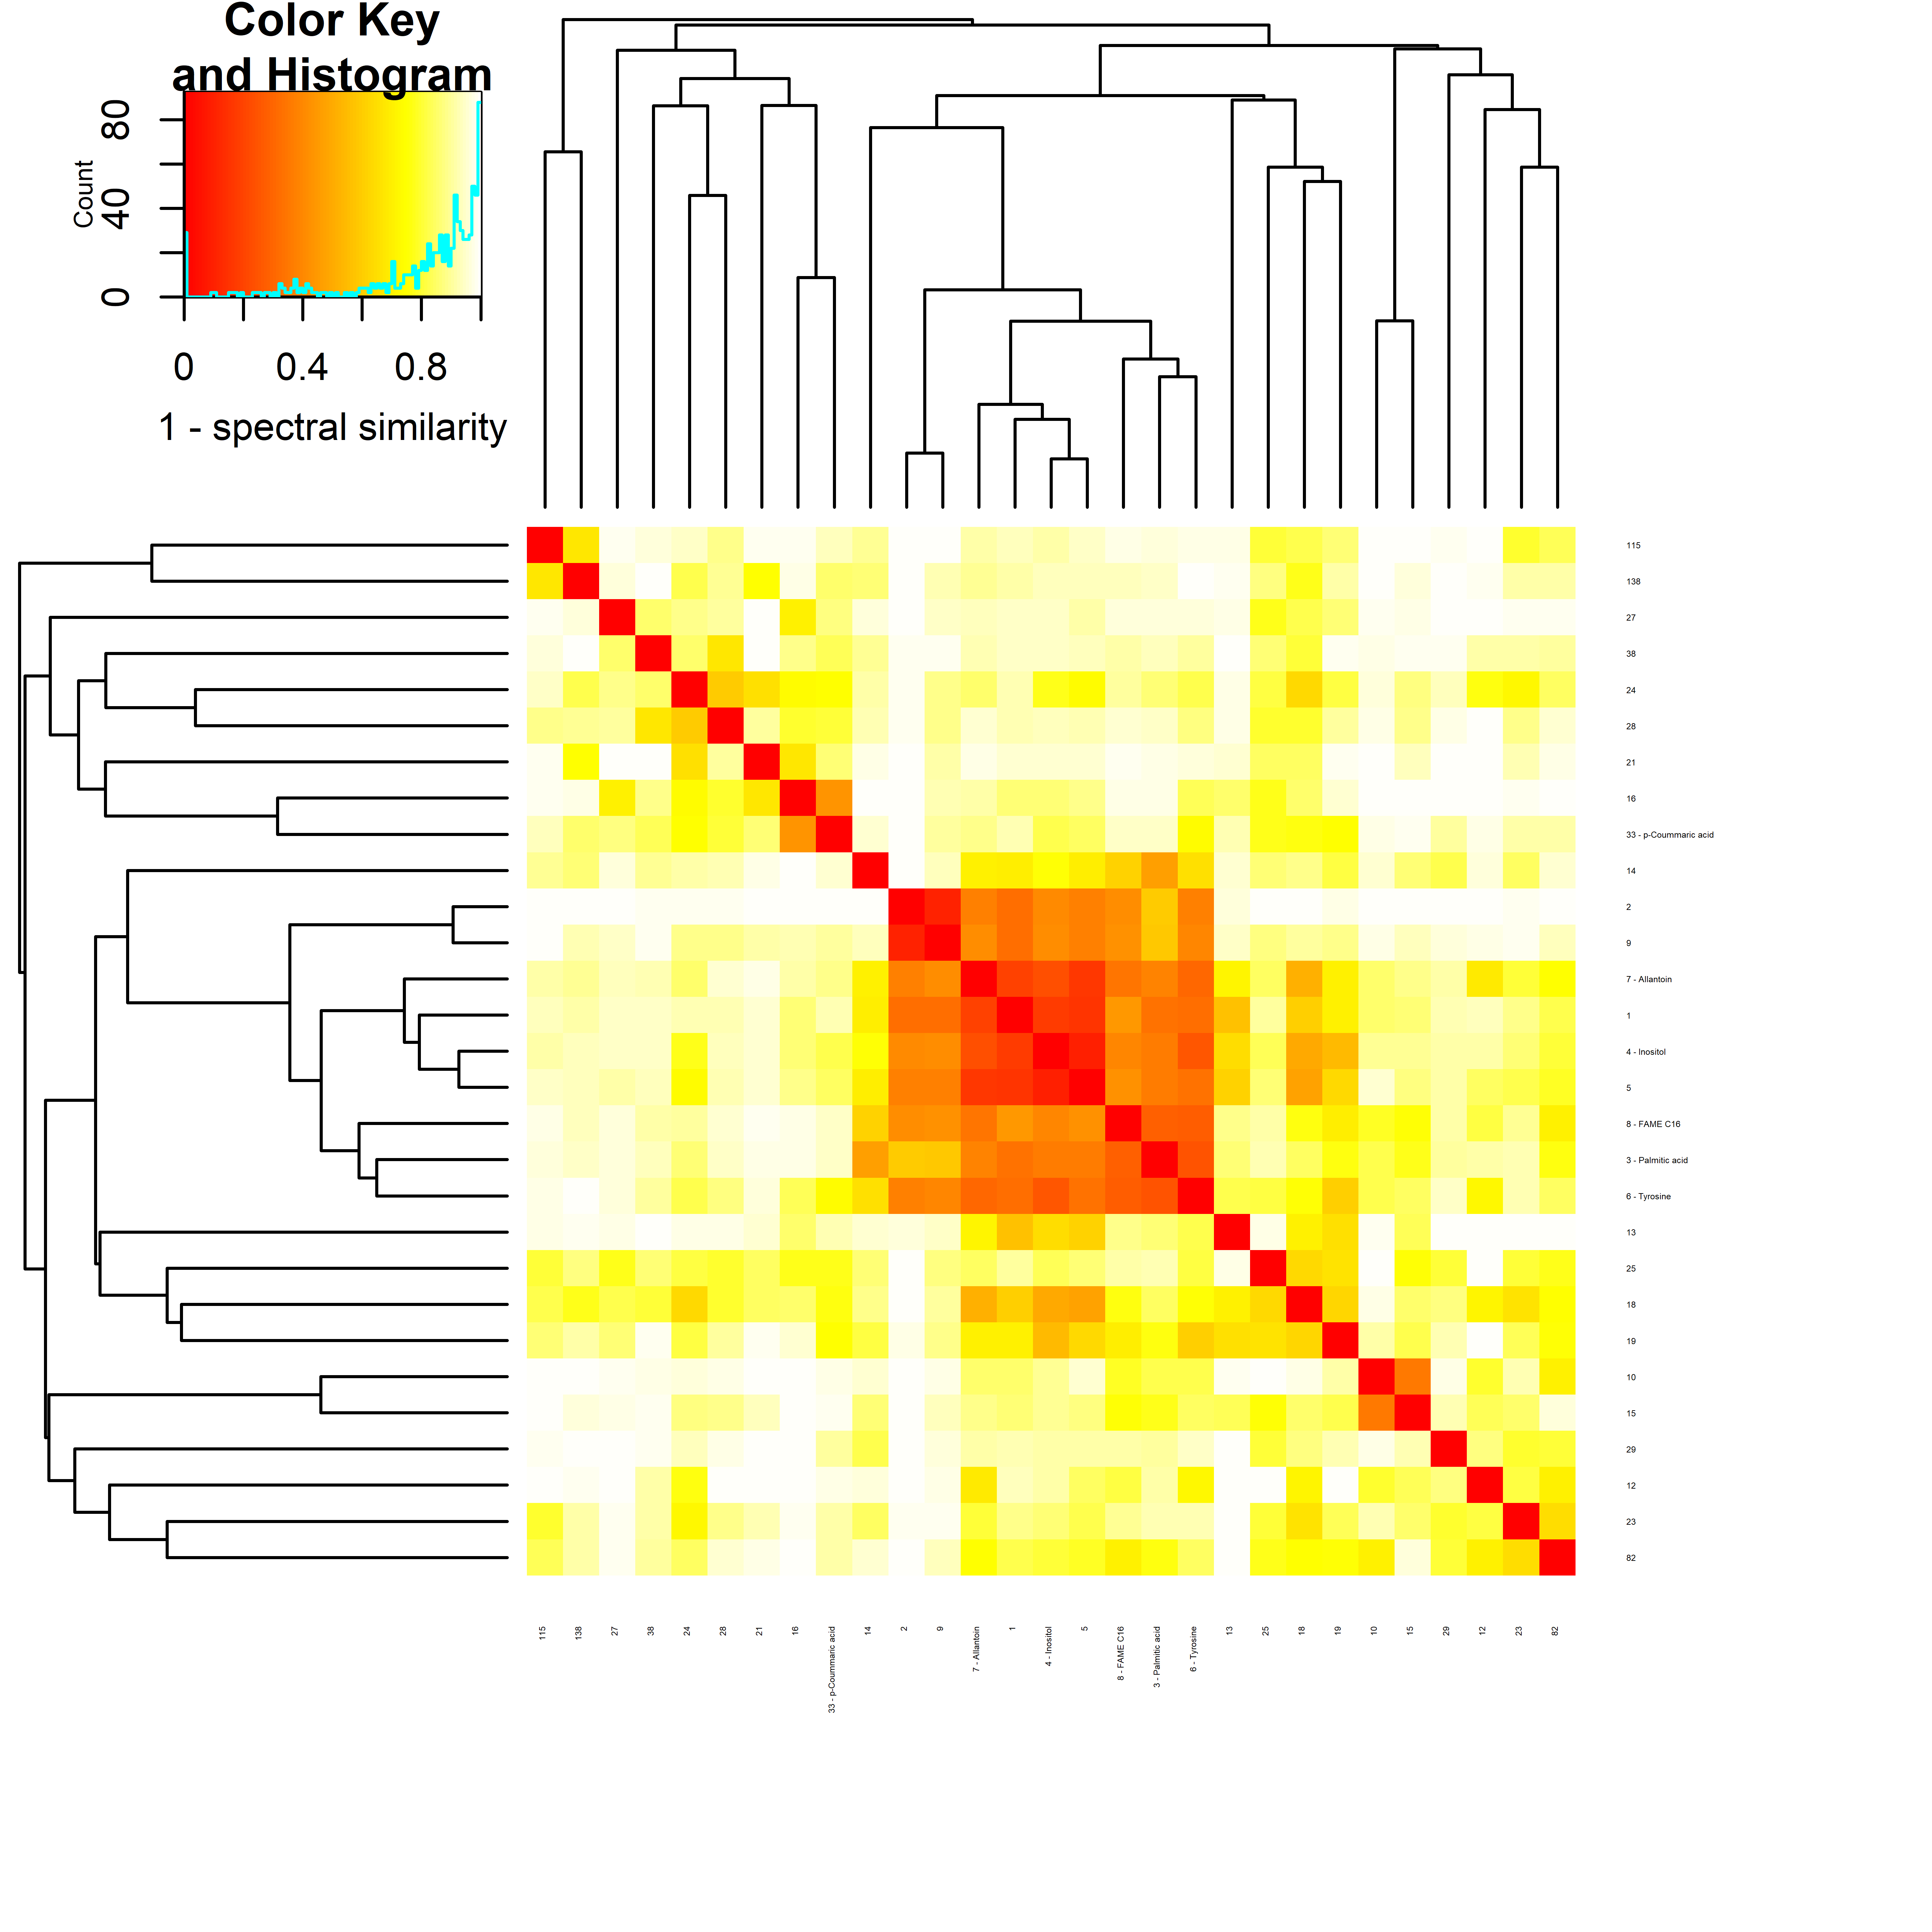
\includegraphics[width=1\linewidth]{heatmap} 

}

\caption{Heatmap.}\label{fig:unnamed-chunk-24}
\end{figure}

\hypertarget{quantitation}{%
\subsection{Quantitation}\label{quantitation}}

Once the spectra werer grouped and identified, the quantification step
will proceed by extracting the intensity of the most intense ion (called
representative ion) of each spectrum to represent the intensity of the
entire spectrum. However, GC-MS analysis often require some sort of
sample preparation that may alter the the representative ion of the
analyte. For example, sample derivatized with trimethylsilyl groups
present the m/z 73 fragment-ion as the most intense in almost every
spectrum, even though they represent the trimethylsilyl groups in the
analyte. For that occurrence, the PipMet asks the user if the samples
were derivatized (Trimethylsilation is currently supported) in order to
avoid the m/z 73 as the representative peak, what would include too much
variation in the the data. Therefore, if the m/z 73 is the most intense,
the second peak will be used as representative.

\begin{figure}

{\centering 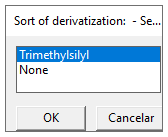
\includegraphics[width=0.5\linewidth]{10} 

}

\caption{Derivatization.}\label{fig:unnamed-chunk-25}
\end{figure}

Another feature for improve the quantification step is to merge or
remove compounds. In derivatization cases, the same compound may be
identified more than once, for the different numbers of trimethylsilyl
groups in the analyte, called derivates. For proper quantification, the
intensity of all derivatives that originated from the same molecule must
be summed in order to represent the real intensity of the analyte. The
user may also remove a compound identified previously from the
quantification, such as contaminantes or column bleeding.

\hypertarget{data-normalization}{%
\subsubsection{Data normalization}\label{data-normalization}}

The PipMet package, through the NormalyzerDE package, offers different
methods of normalization so that the user can choose the best to addapt
to the data after evaluation the models and the printed report. For the
normalization to occur, the user must point the category from which the
samples are better grouped. For the example, select `group'.

\begin{figure}

{\centering 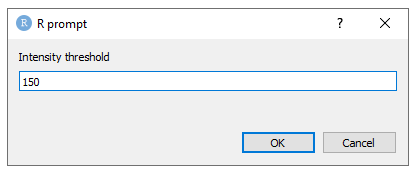
\includegraphics[width=0.5\linewidth]{7} 

}

\caption{Groups for normalization.}\label{fig:unnamed-chunk-26}
\end{figure}

The normalyzerDE R package provides different normalization methods and
a report with metrics for the user to pick the best normalization that
fit his data. In the Example, a folder `Normalyzer\_results' is created
and the user is invited to look at the pdf report and to choose among
the methodologies. Here, we picked the CycLoess normalization. Then a
histogram of the variance and standard deviation is plot in the
`Statistics' folder, along with a boxplot of the same metrics and its
outliers.

\begin{figure}

{\centering 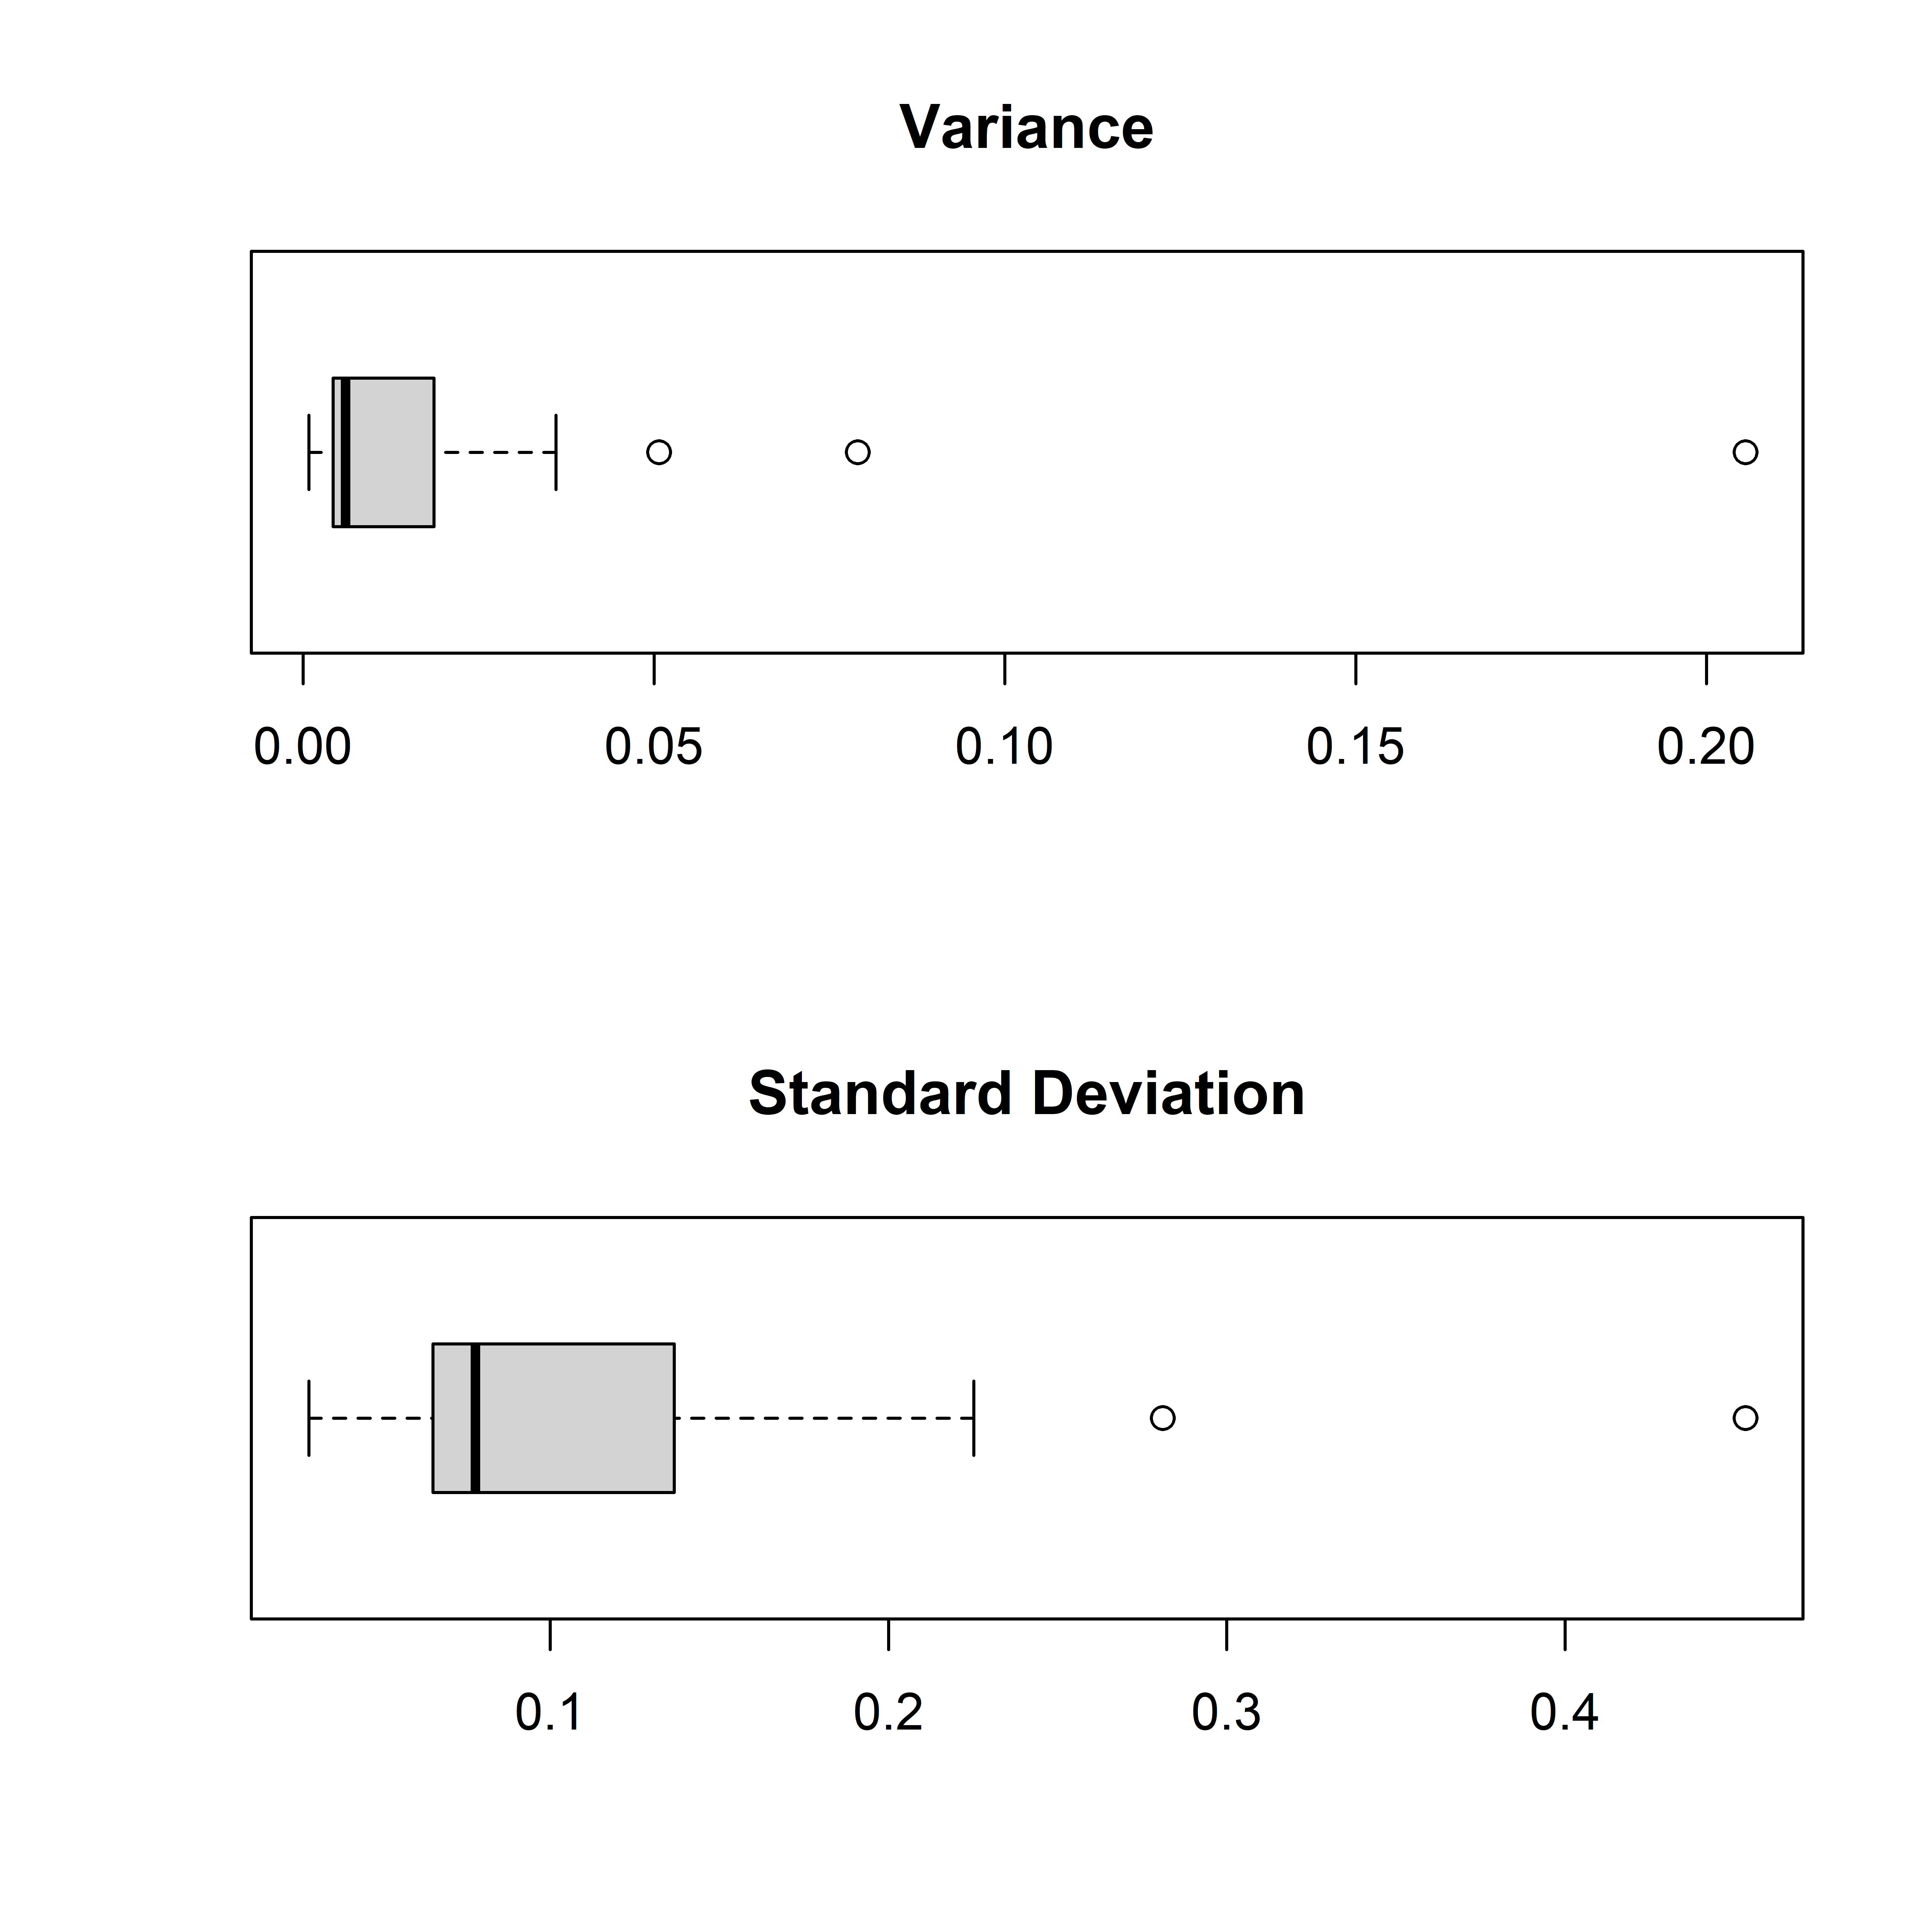
\includegraphics[width=1\linewidth]{boxplot} 

}

\caption{Boxplot, variance and standard deviation.}\label{fig:unnamed-chunk-27-1}
\end{figure}
\begin{figure}

{\centering 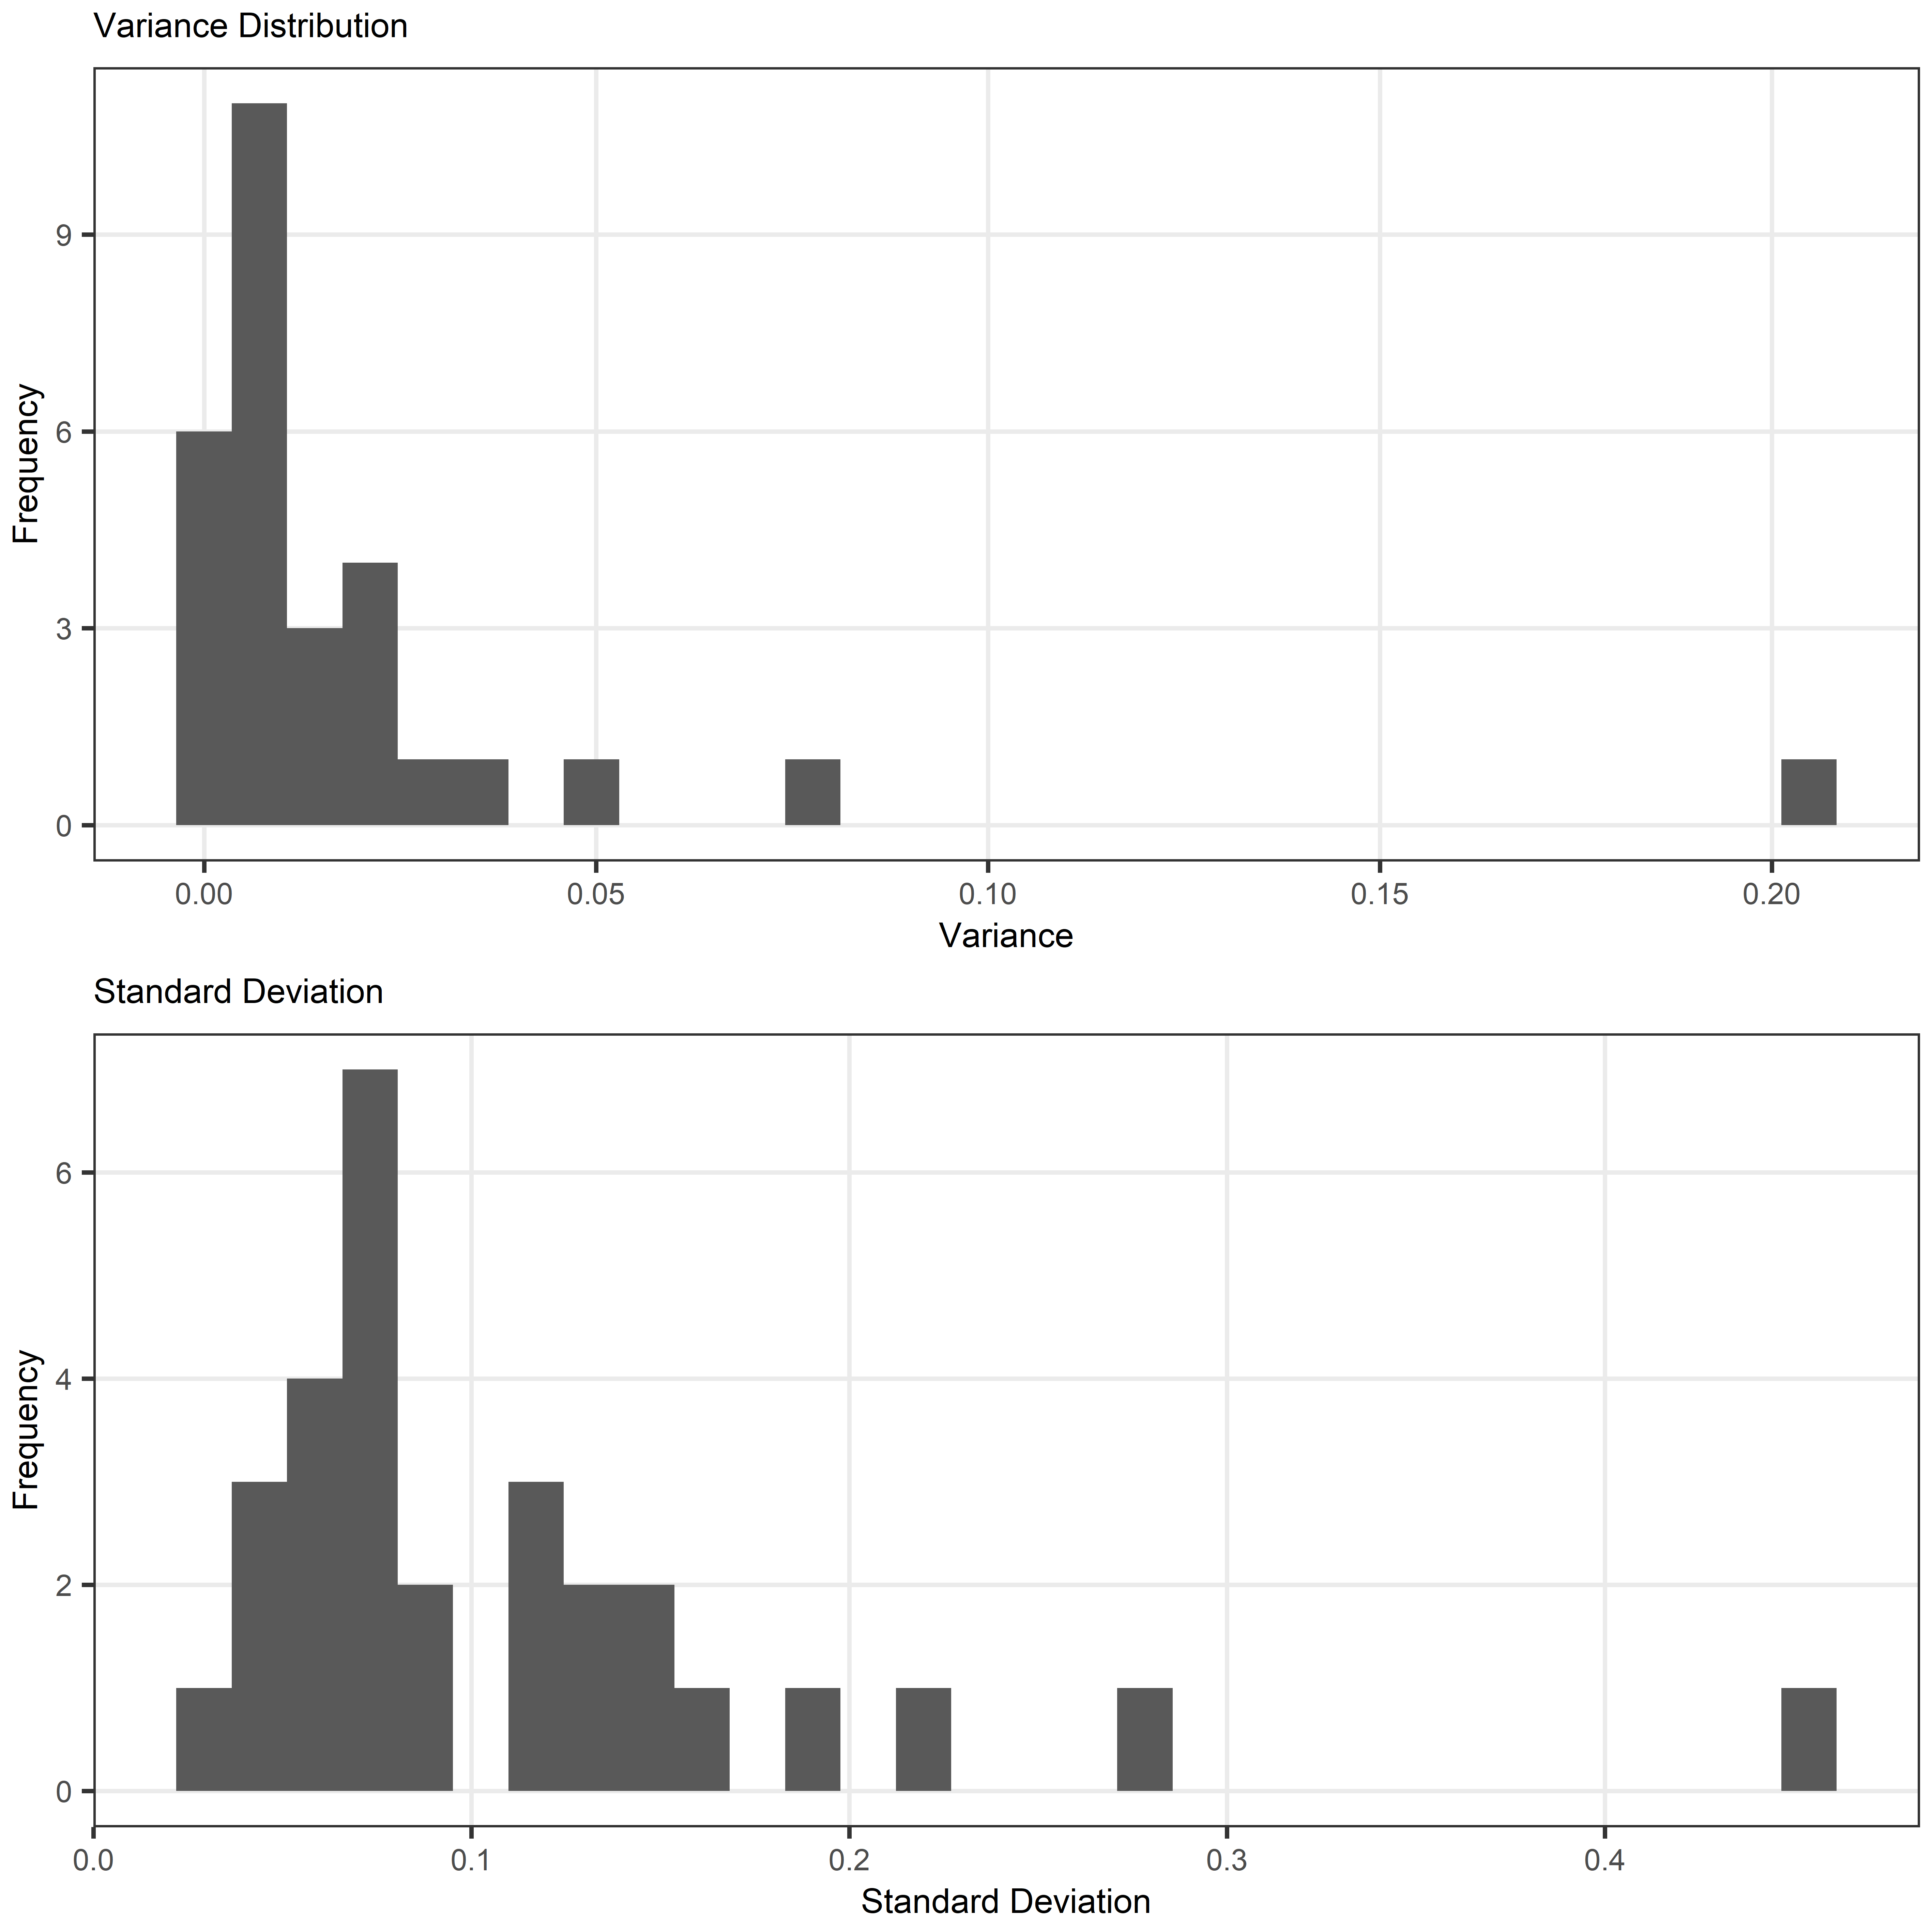
\includegraphics[width=1\linewidth]{variance_dp} 

}

\caption{Boxplot, variance and standard deviation.}\label{fig:unnamed-chunk-27-2}
\end{figure}

The variance and standard deviation is calculated from the intensities
of the representative ion and the second most intense in each of the
spectra. If the spectra is not correctly proposed (for example, if it
has a coelution not detected), the rate between the representative peak
and the second most intense will not be stable along the samples where
the compound appears, showing too much variance and standard deviation.
The same may happen to bleeders or contaminants. Therefore, the user
must monitor those results in order to have variance and standard
deviation (sd) as low as possible. If some compound present high
variance or sd, the user may choose to remove outliers in general (shown
in the boxplot image) ou remove compounds with variance bigger than a
threshold. For the example, the CycLoess normalization is enough and it
won't be necessary to remove outliers ou any compound.

\begin{figure}

{\centering 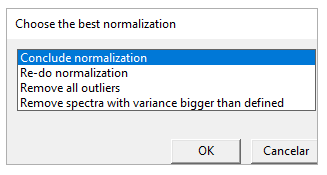
\includegraphics[width=0.3\linewidth]{13} 

}

\caption{Normalization check.}\label{fig:unnamed-chunk-28-1}
\end{figure}
\begin{figure}

{\centering 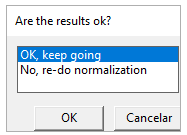
\includegraphics[width=0.3\linewidth]{14} 

}

\caption{Normalization check.}\label{fig:unnamed-chunk-28-2}
\end{figure}

Further on, the user is asked which column from the metadata table
represents the replicate column, if there is any. For the example files,
that information is also represented by the `group' column.

\begin{figure}

{\centering 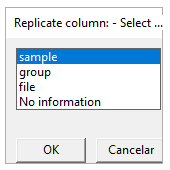
\includegraphics[width=0.25\linewidth]{15} 

}

\caption{Replicate information.}\label{fig:unnamed-chunk-29}
\end{figure}

\hypertarget{statistics-figures}{%
\subsubsection{Statistics Figures}\label{statistics-figures}}

After the quantification step is completed, it is plotted the figures
regarding the statistics step of the workflow. They are: volcano plots,
heatmaps and PCA. The first is volcano. The user is instructed to select
a condition from the metadata table to compare two characteristics from
that condition. Here, we choose `group' to compare the `Energy' and
`Sugar' compounds.

\begin{figure}

{\centering 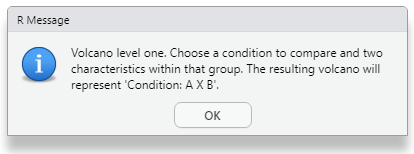
\includegraphics[width=0.3\linewidth]{16} 

}

\caption{Volcano setup.}\label{fig:unnamed-chunk-30-1}
\end{figure}
\begin{figure}

{\centering 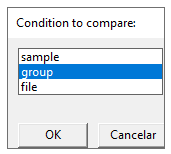
\includegraphics[width=0.3\linewidth]{17} 

}

\caption{Volcano setup.}\label{fig:unnamed-chunk-30-2}
\end{figure}
\begin{figure}

{\centering 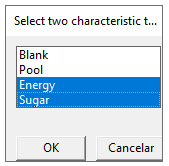
\includegraphics[width=0.3\linewidth]{18} 

}

\caption{Volcano setup.}\label{fig:unnamed-chunk-30-3}
\end{figure}

If more than one category to describe the samples are availabe, the user
may do a Level 2 volcano plot, to compare using to describers. Such as
`Energy: Control X Treatment' and `Sugar: Control X Treatment'.

Along with each of the comparison for plotting the Volcano plot, a file
containing the p-value (significance) and foldchange of the comparisons
is written inside the volcano plot folder.

\begin{figure}

{\centering 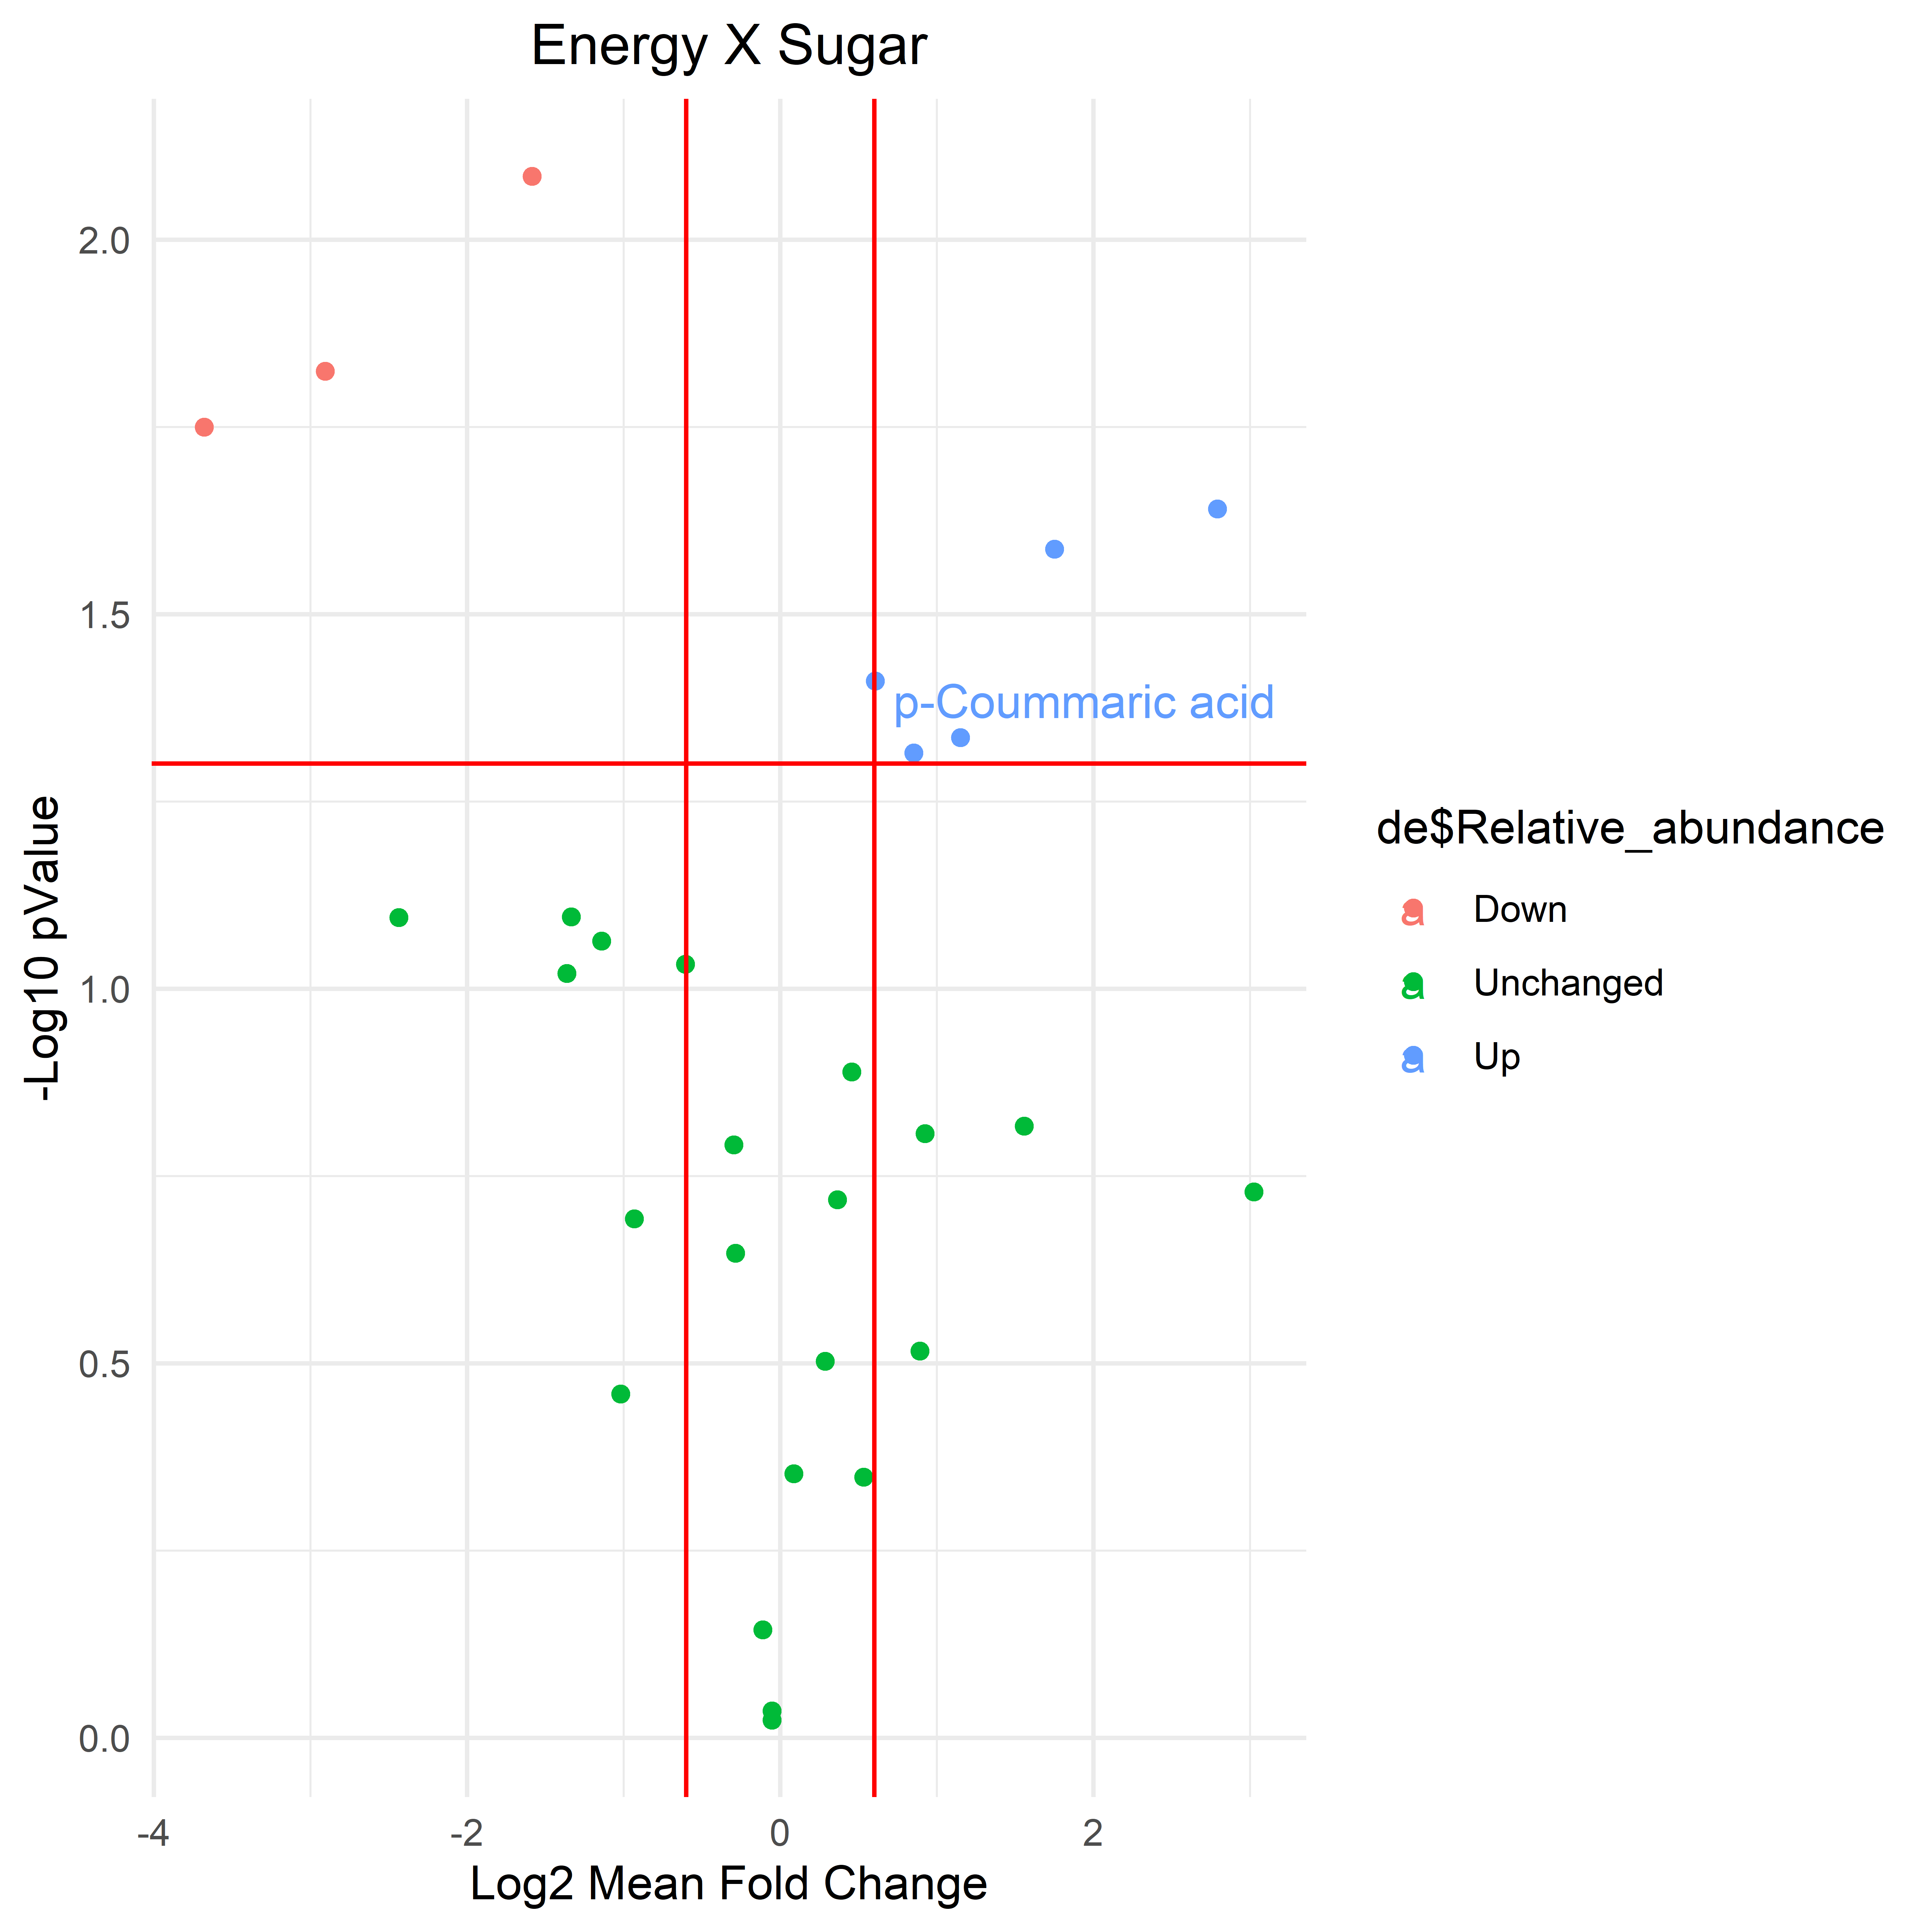
\includegraphics[width=0.4\linewidth]{volcano_identified} 

}

\caption{Volcano plot.}\label{fig:unnamed-chunk-31}
\end{figure}

Next, the PCA of all samples are plotted, using all spectra proposed.

\begin{figure}

{\centering 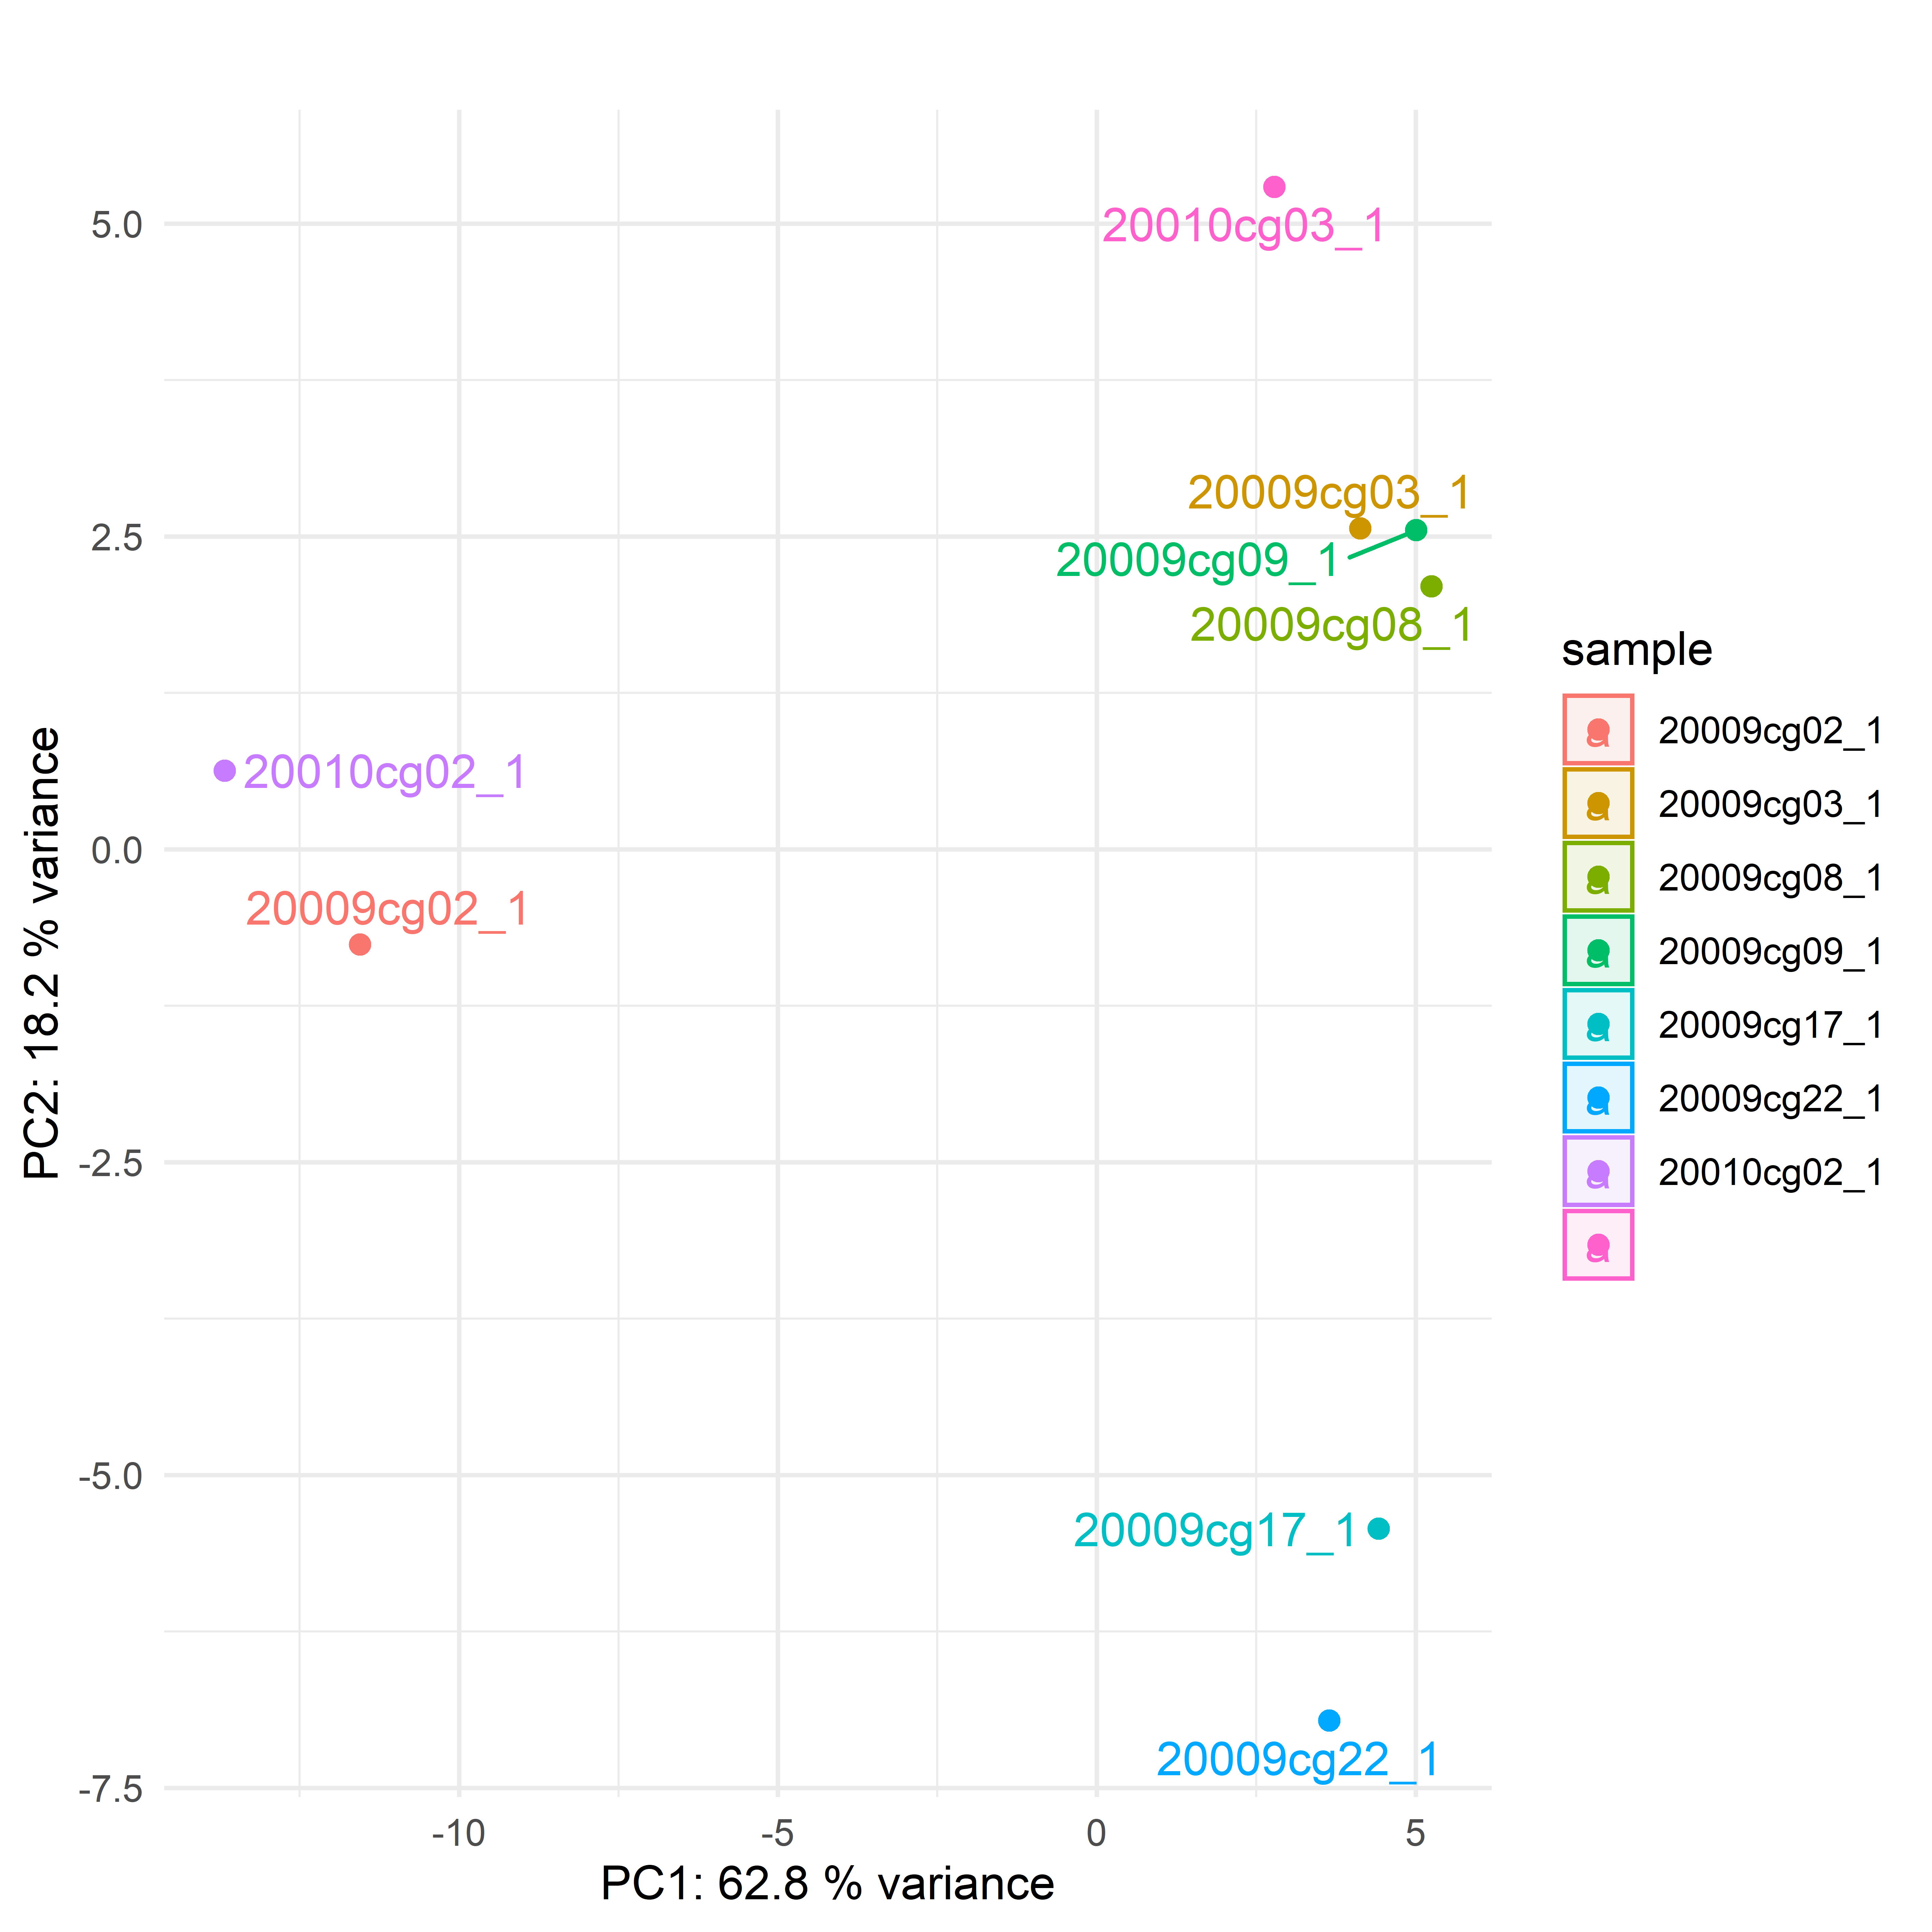
\includegraphics[width=0.4\linewidth]{PCA_named_sample} 

}

\caption{PCA of samples.}\label{fig:unnamed-chunk-32}
\end{figure}

The user is then asked to choose a particular condition to plot the PCA
for specified samples only. For example, we choose to only look at
Sugarcane and Energycane samples, therefore, we choose `group' and
select both `Sugar' and `Energy' describers.

\begin{figure}

{\centering 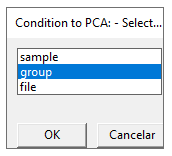
\includegraphics[width=0.25\linewidth]{19} 

}

\caption{PCA selected samples.}\label{fig:unnamed-chunk-33}
\end{figure}
\begin{figure}

{\centering 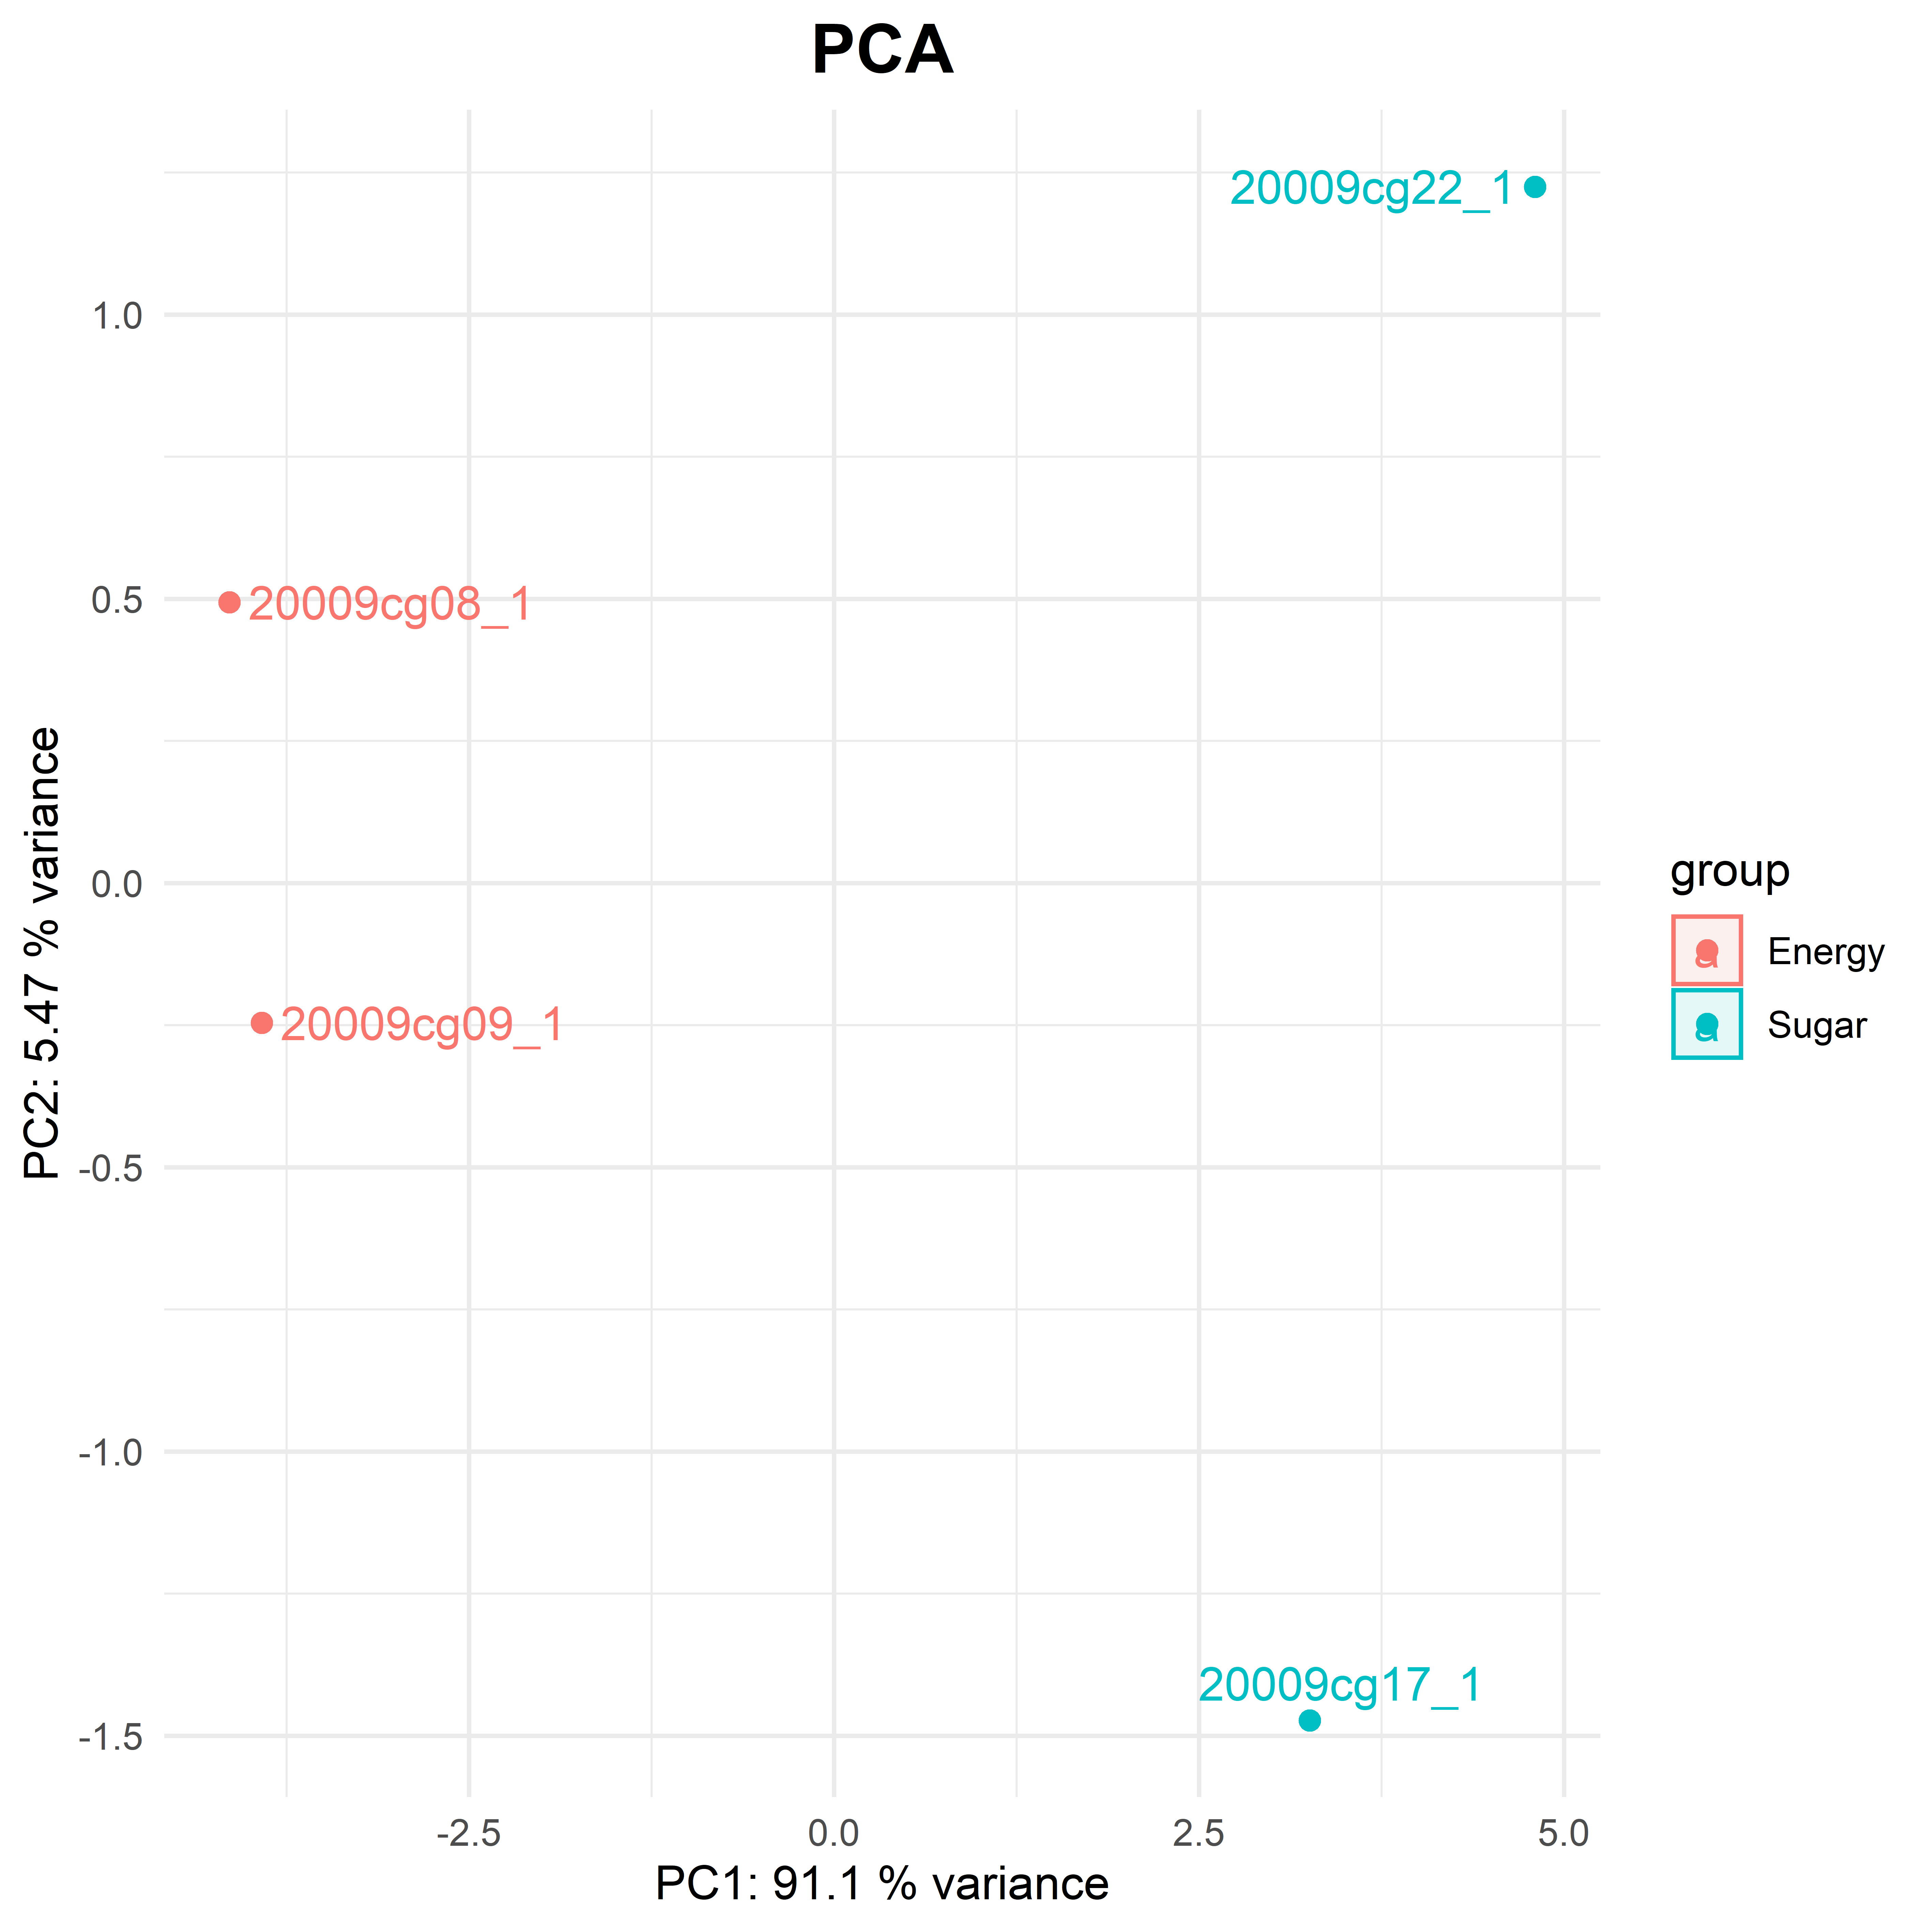
\includegraphics[width=0.5\linewidth]{PCAselected_named_group} 

}

\caption{PCA of selected samples.}\label{fig:unnamed-chunk-34}
\end{figure}

The PCA is plotted again only for the identified compounds, this time,
repeating the some process as before: plot of all samples and asking for
specific samples.

\begin{figure}

{\centering 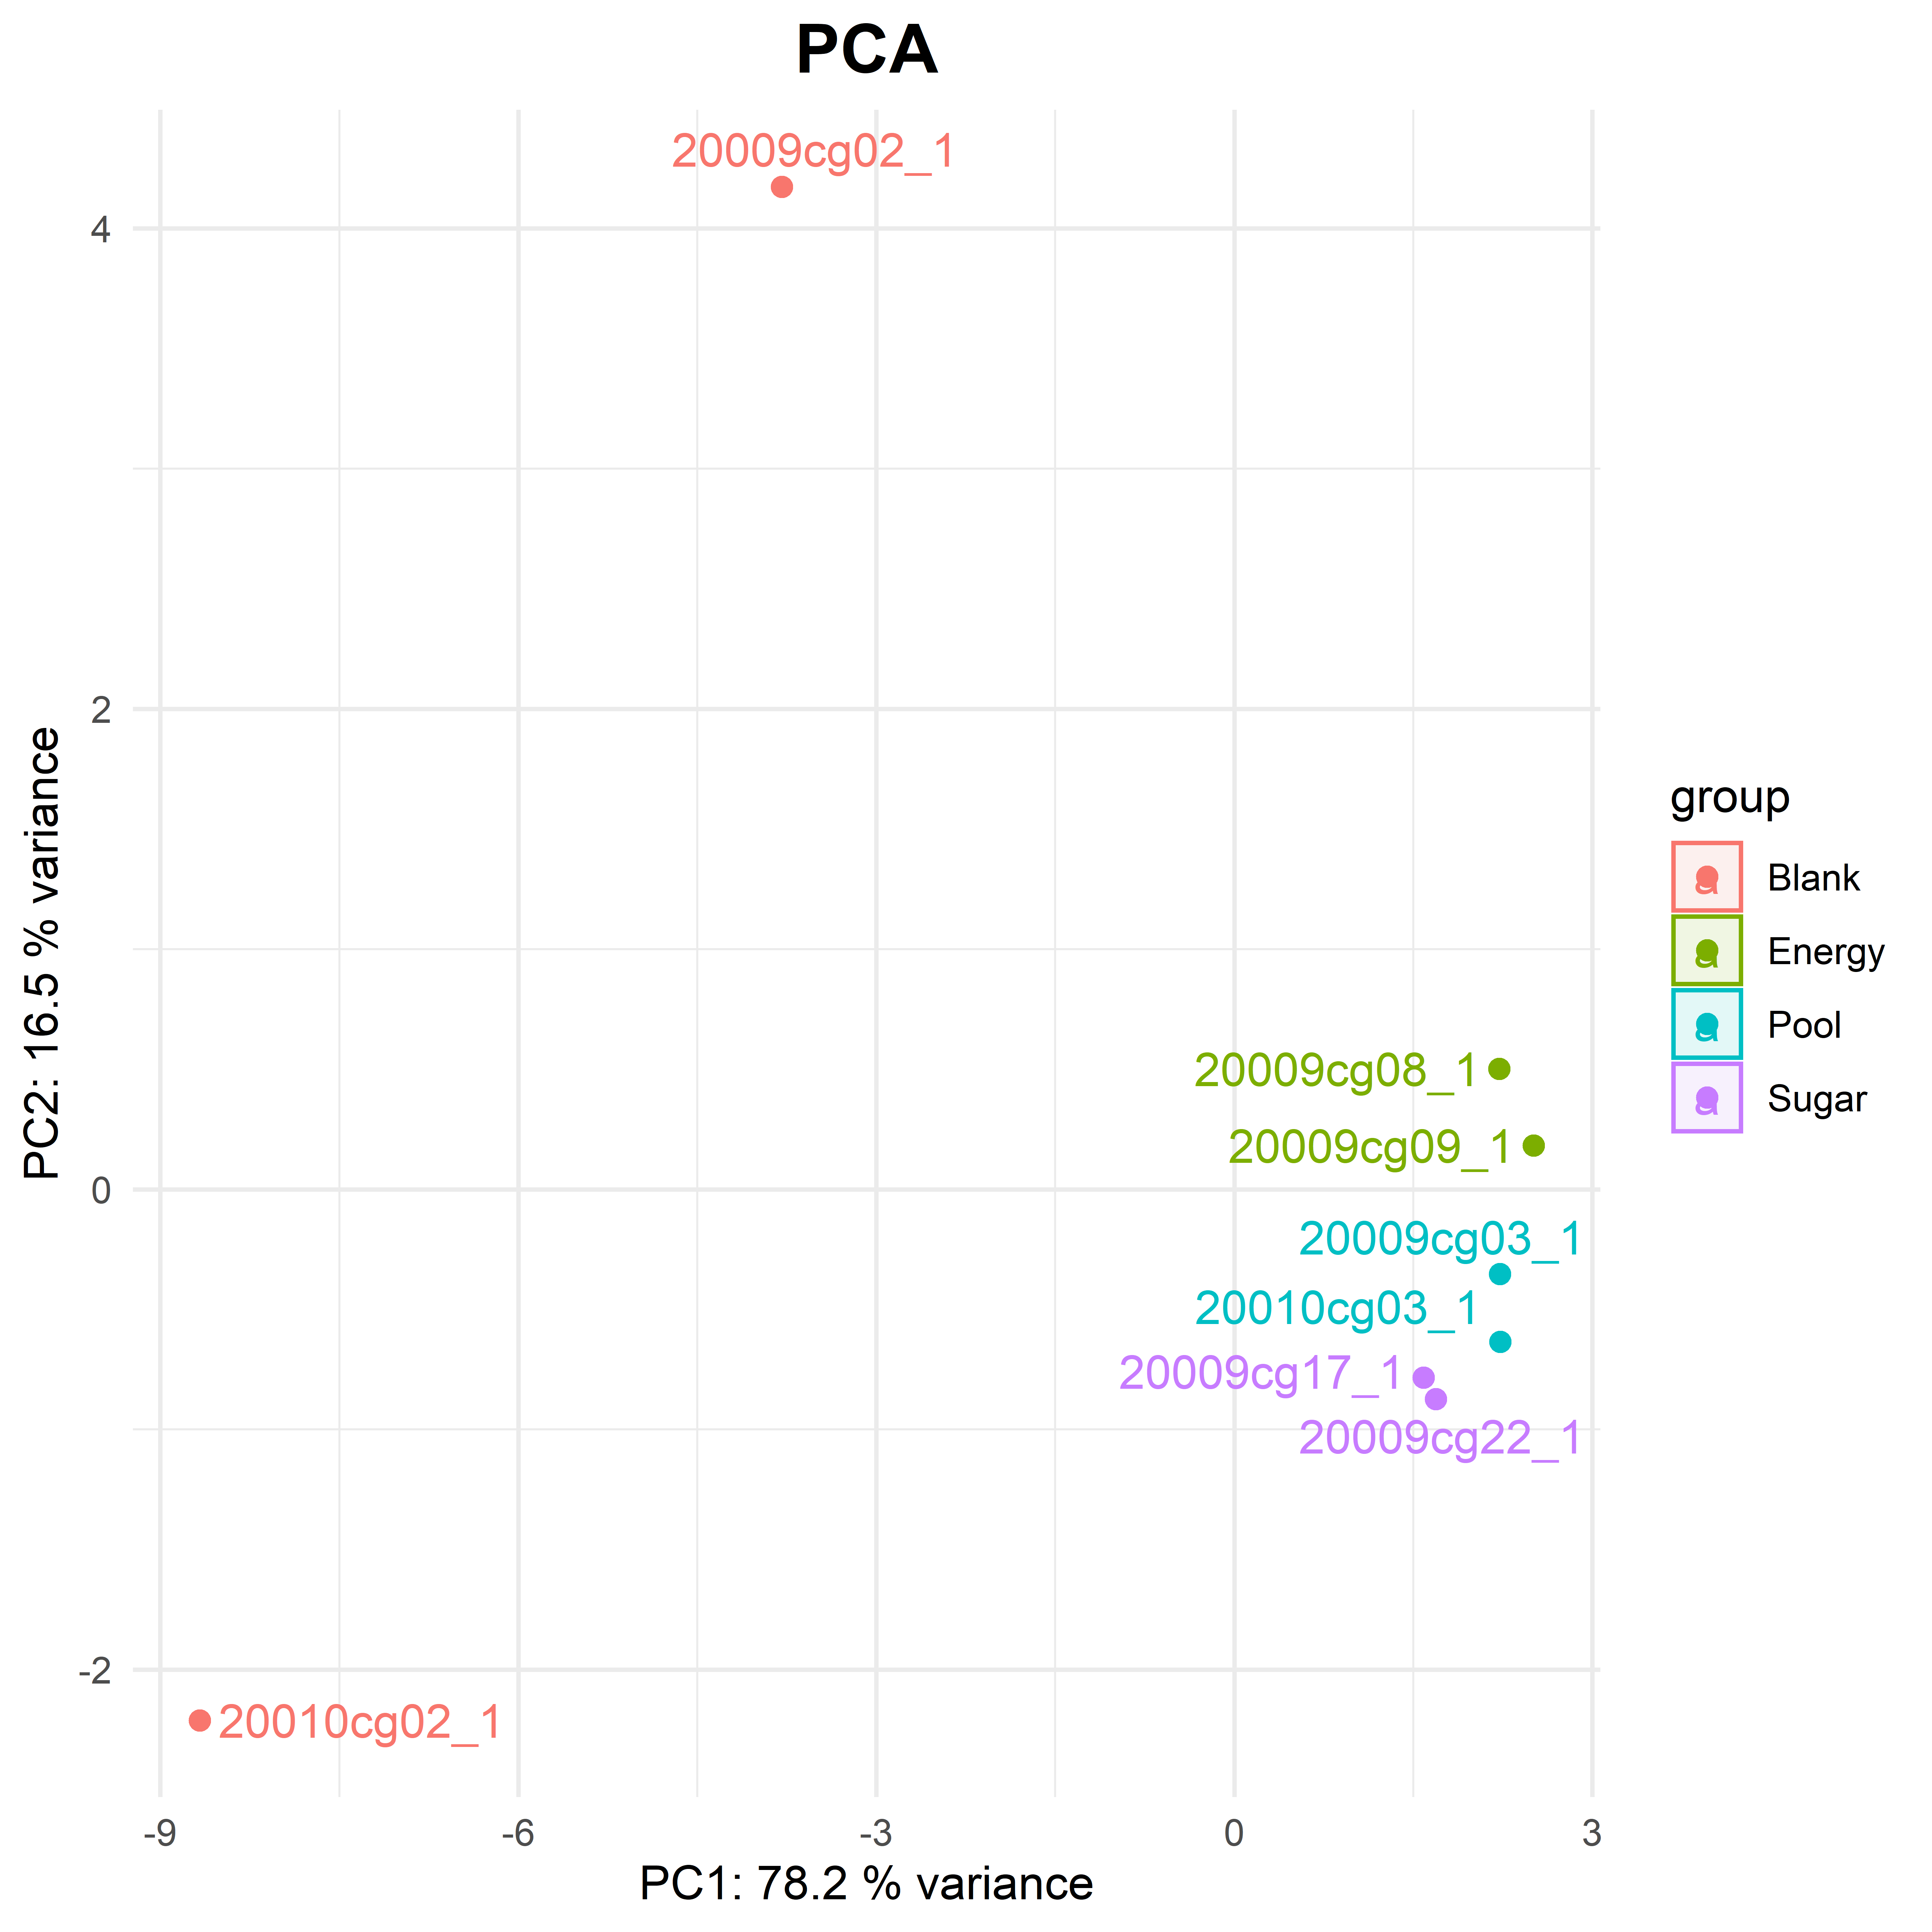
\includegraphics[width=0.5\linewidth]{PCA_named_group_identified} 

}

\caption{PCA of all samples - Identified compounds only.}\label{fig:unnamed-chunk-35}
\end{figure}
\begin{figure}

{\centering 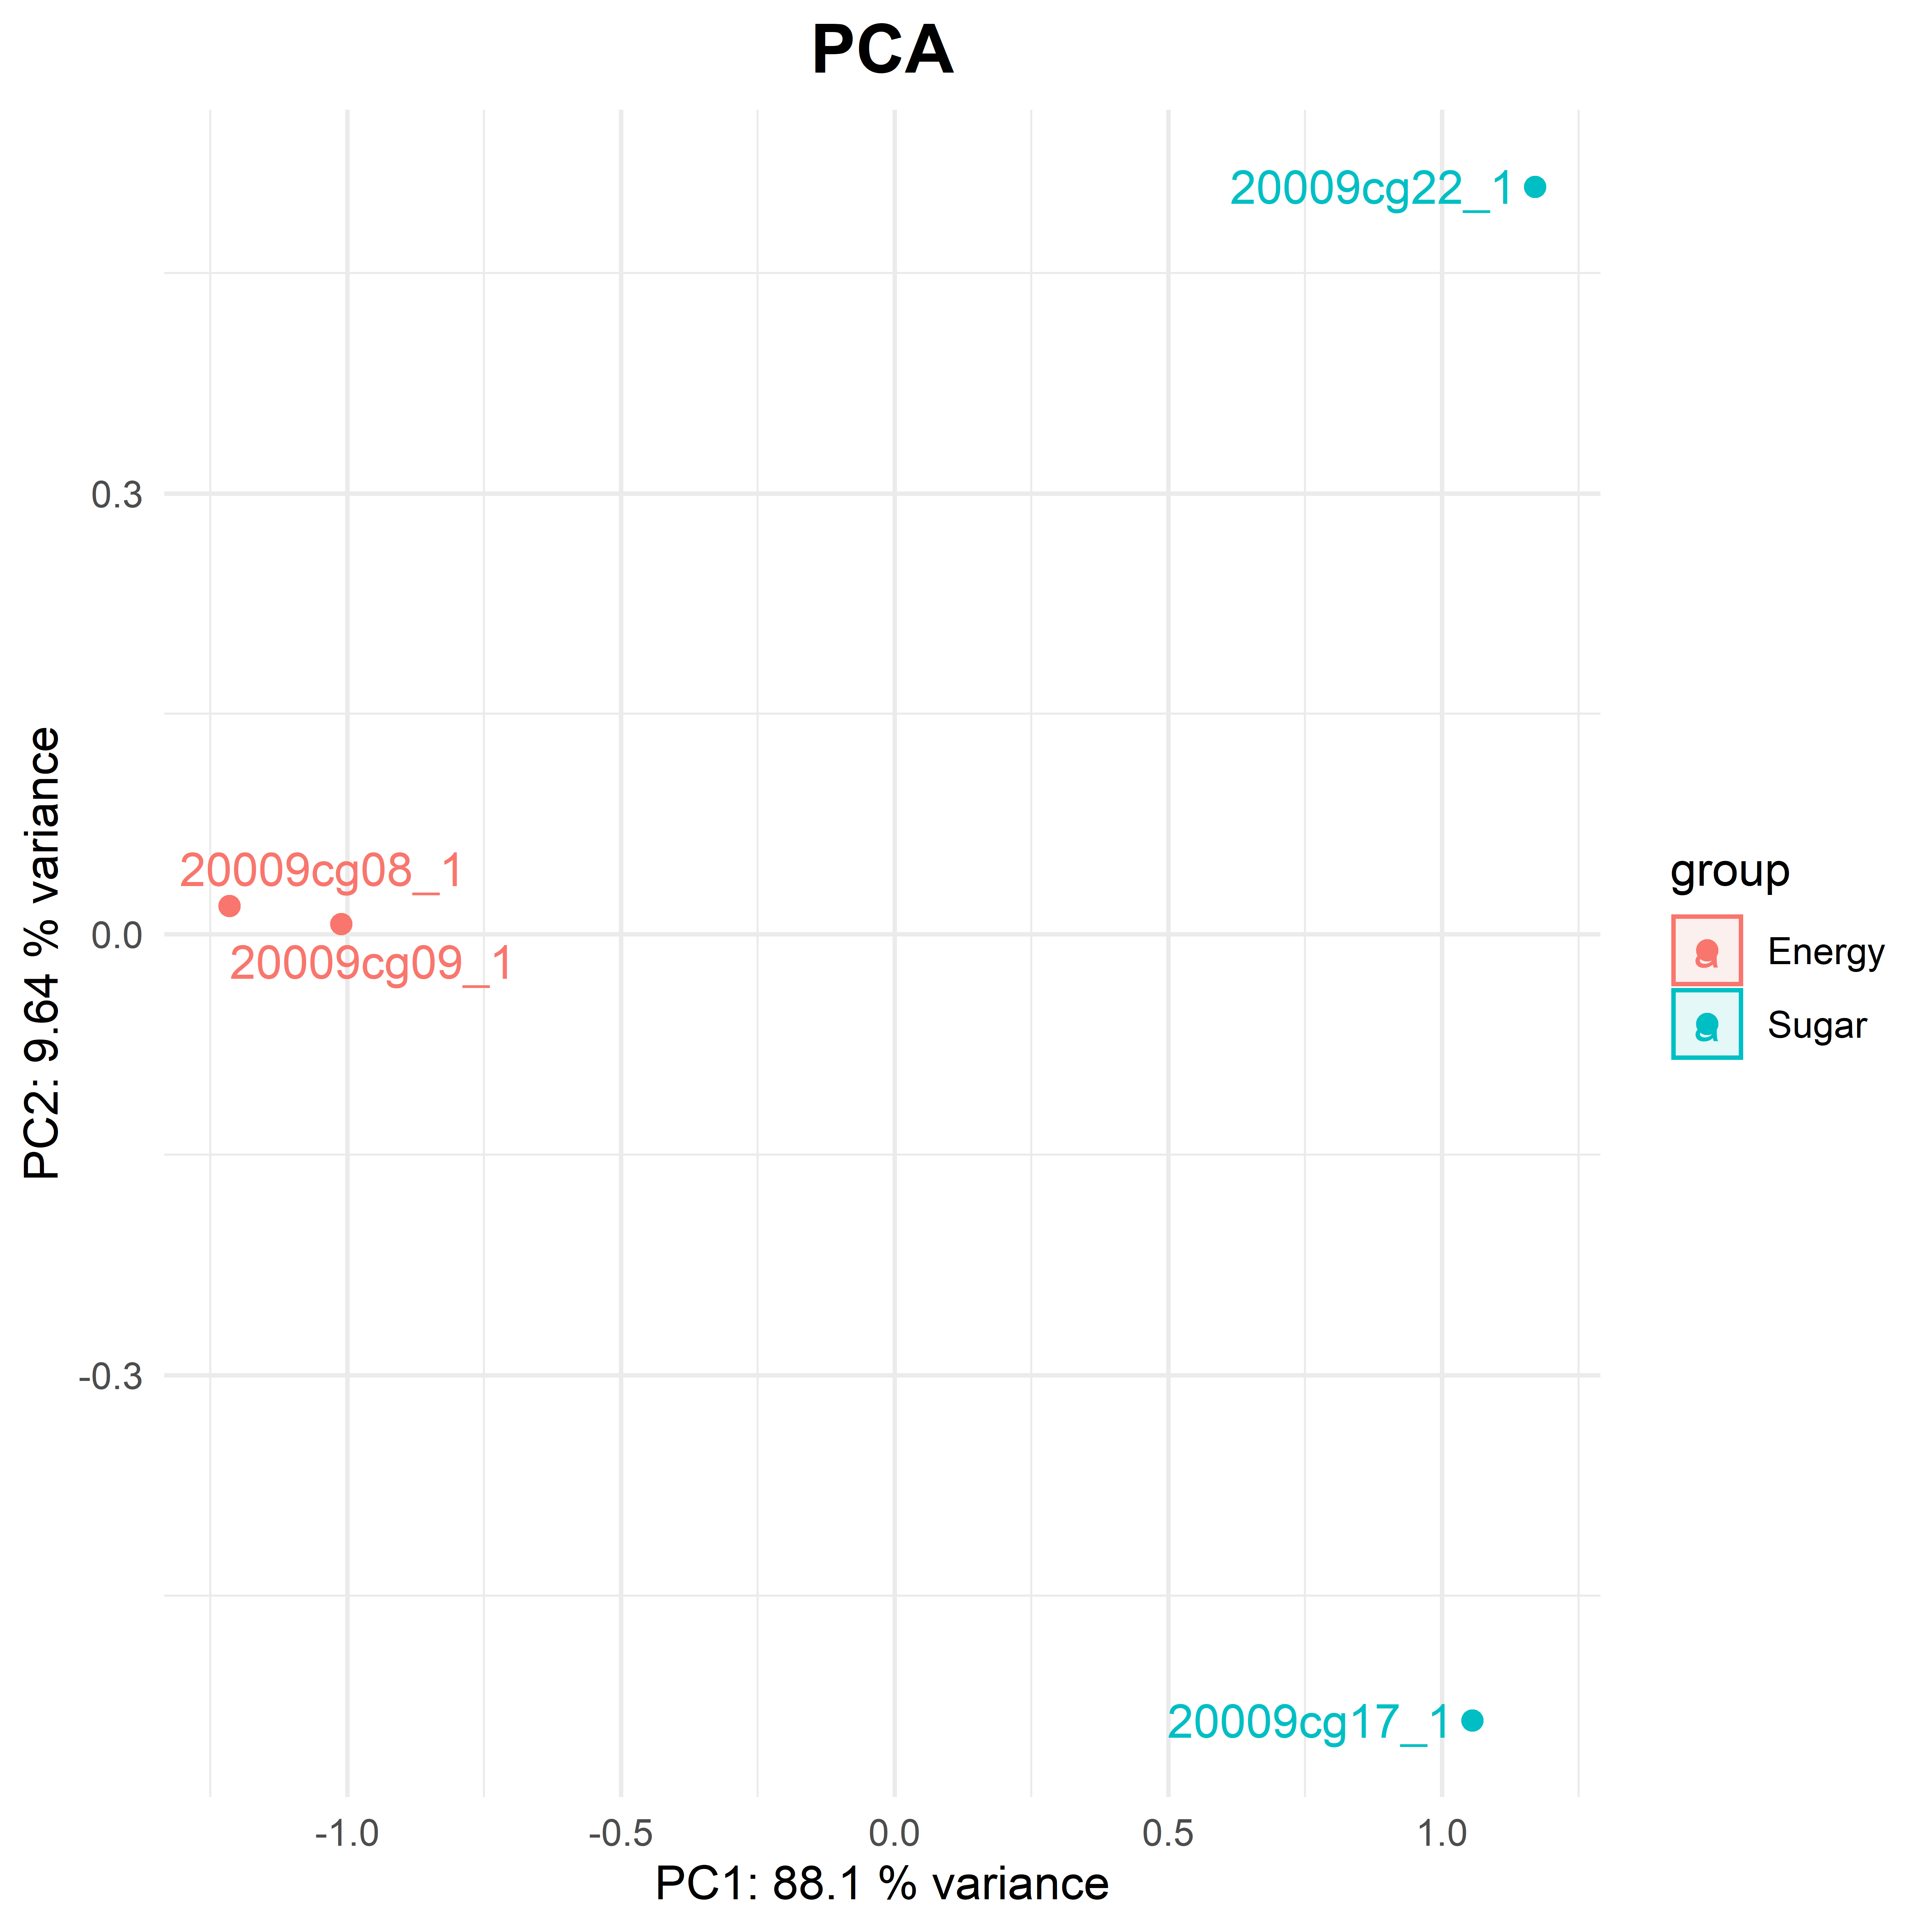
\includegraphics[width=0.5\linewidth]{PCAselected_named_group_identified} 

}

\caption{PCA of selected samples - Identified compounds only.}\label{fig:unnamed-chunk-36}
\end{figure}

The heatmaps are plotted colored by the different categories describing
the samples and to plot them, the user is asked how the samples should
be named if the pictures.

\begin{figure}

{\centering 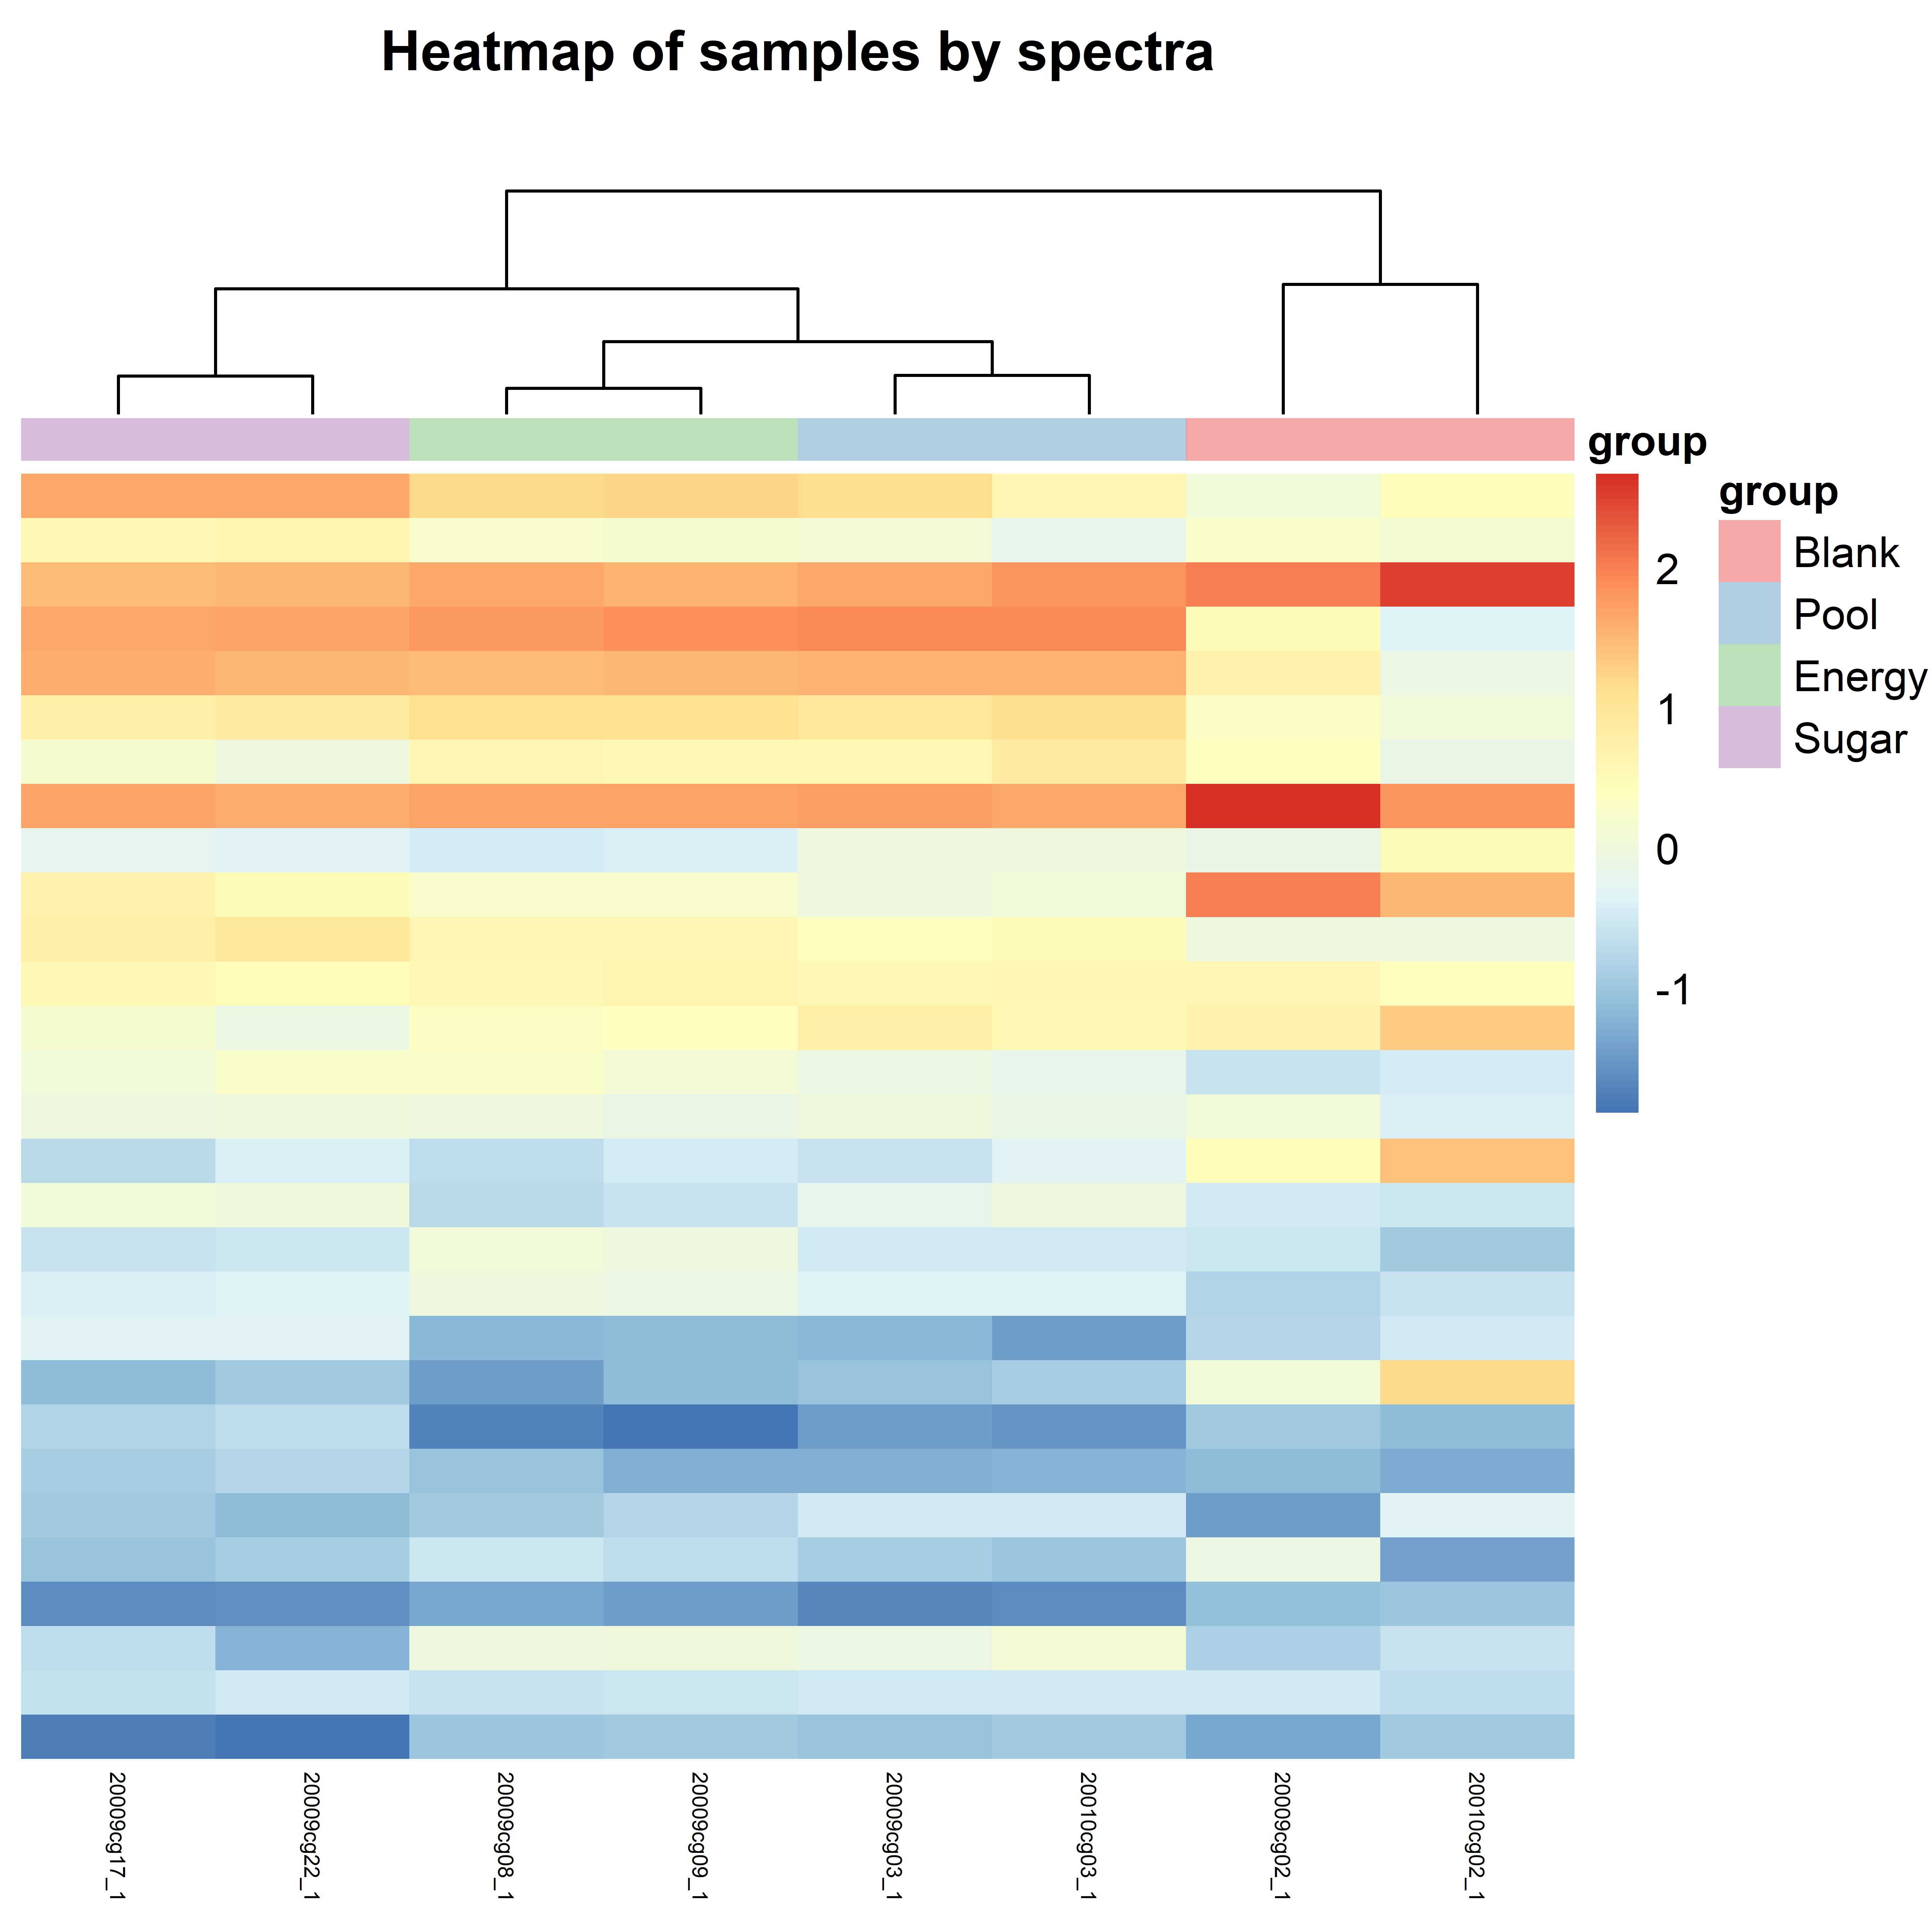
\includegraphics[width=0.6\linewidth]{group_heatmap_scaled_geral} 

}

\caption{Heatmaps of all spectra generated.}\label{fig:unnamed-chunk-37}
\end{figure}
\begin{figure}

{\centering 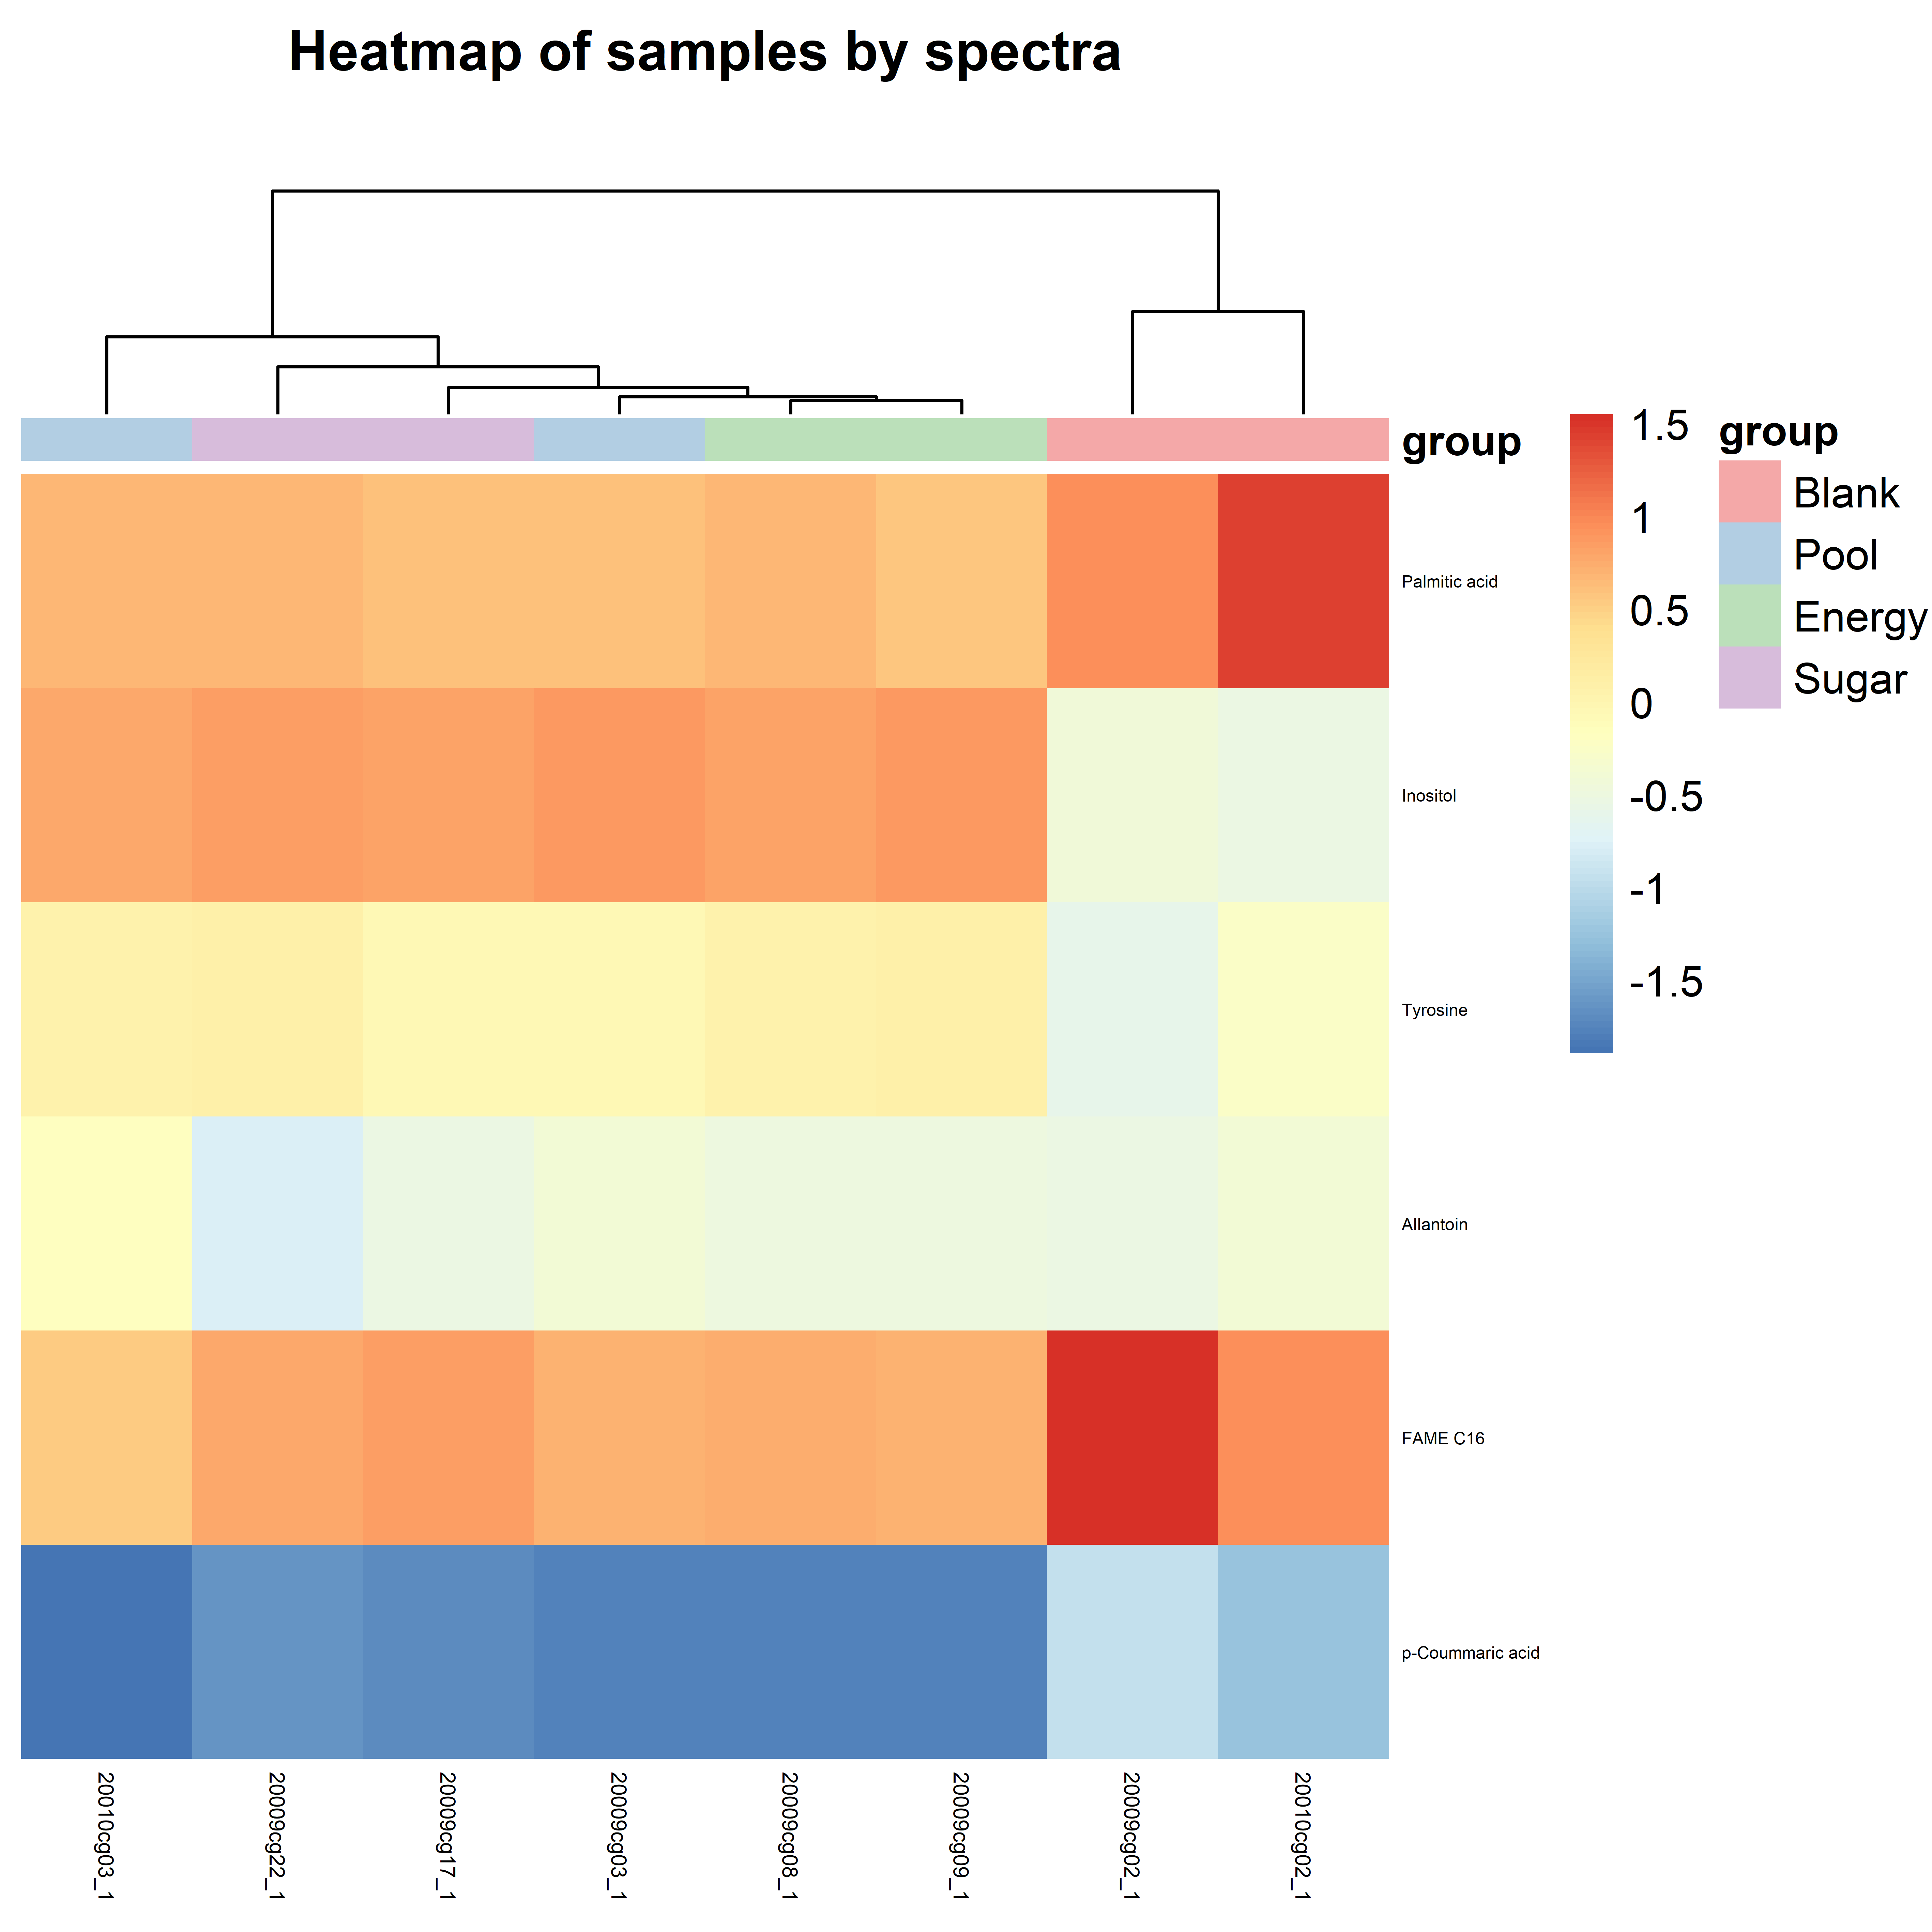
\includegraphics[width=0.6\linewidth]{heatmap_scaled_ident_group_} 

}

\caption{Heatmap of identified spectra only.}\label{fig:unnamed-chunk-38}
\end{figure}
\begin{figure}

{\centering 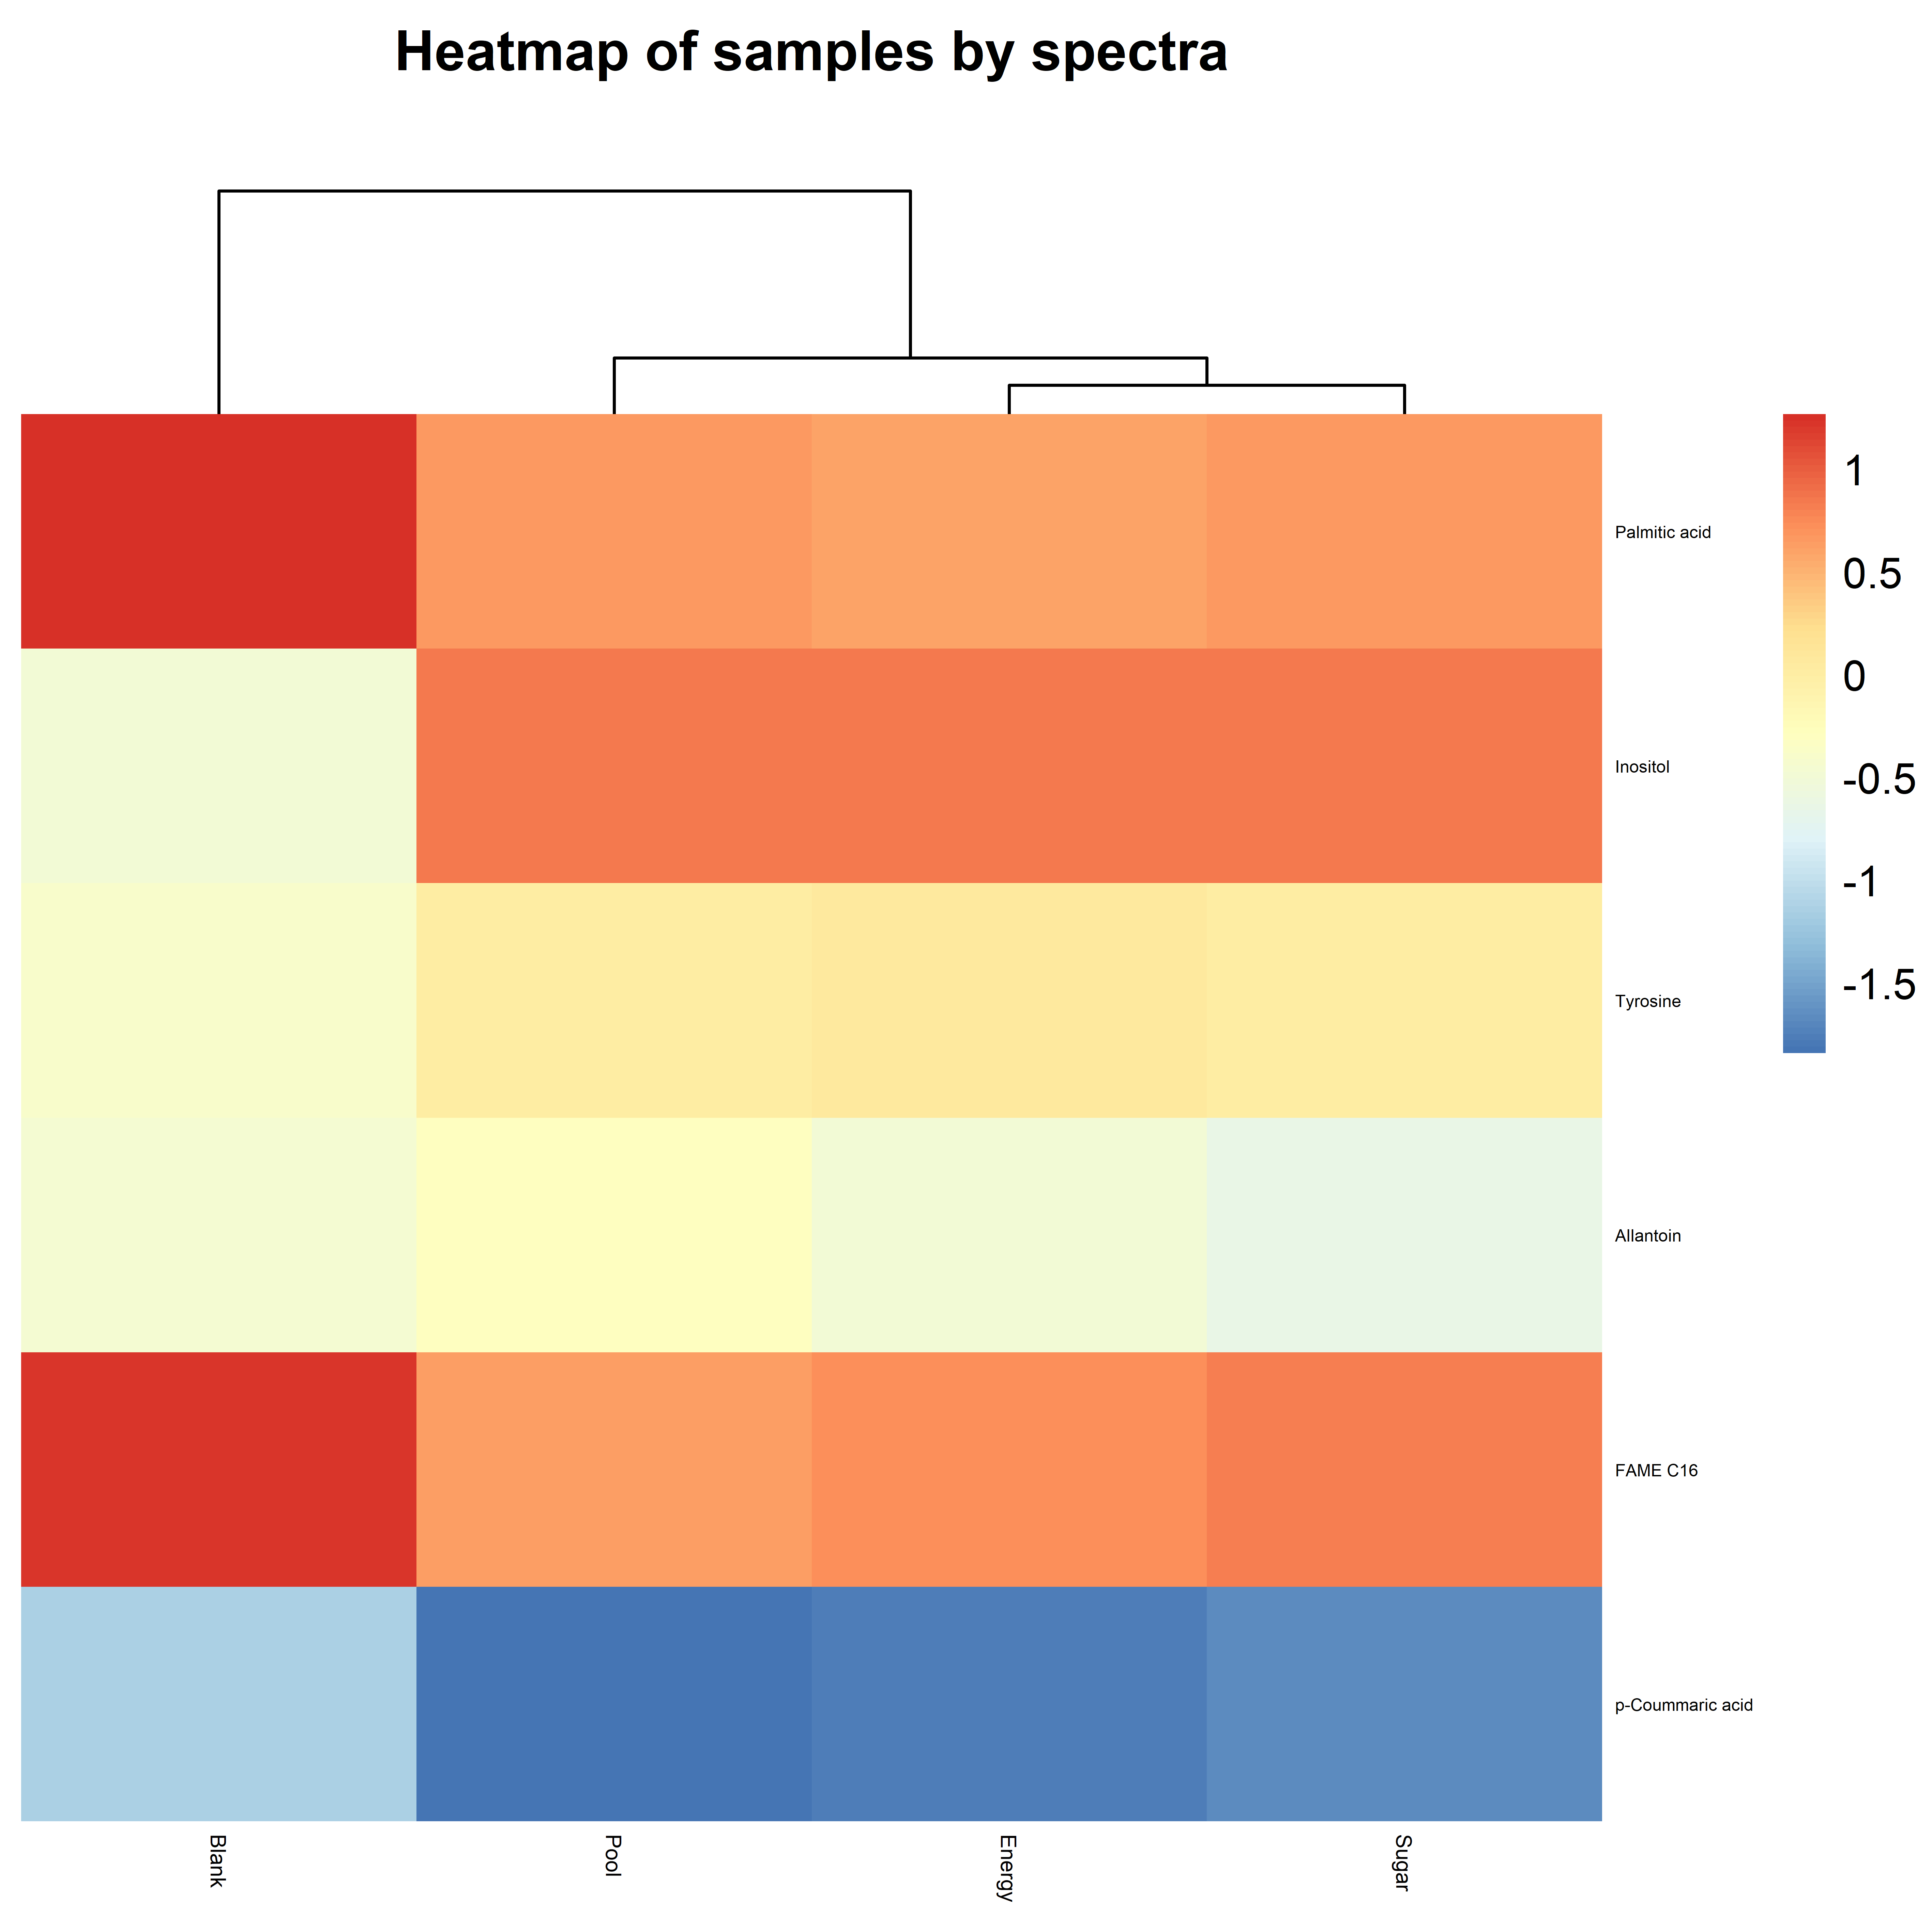
\includegraphics[width=0.6\linewidth]{heatmap_repMean_scaled_ident_unique} 

}

\caption{Heatmap of identified spectra with samples as the mean of their replicates.}\label{fig:unnamed-chunk-39}
\end{figure}

The aforementioned pictures are all generated and saved inside the
project folder, along with the normalization results, such as the
quantification table normalized and not-normalized, including the
variance and standard deviation for the first one. The time and memory
consumption may vary due to the size of the processing data, image
format file chosen along with the decision to generate them, the
parallelization mode and numbers of cores used, among other things.

The pop-ups only appear if the user do not specify the information
required in the parameters of the main function. If everything is given
prior to the beginning of the processing, the function will work without
any intervention or pop-up. For the parameters, refer to the
\texttt{PipMet} documentation.

\begin{figure}

{\centering 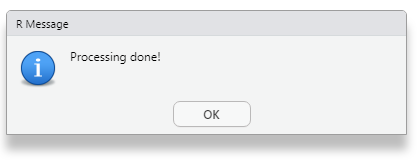
\includegraphics[width=0.4\linewidth]{20} 

}

\caption{Processing done.}\label{fig:unnamed-chunk-40}
\end{figure}

\hypertarget{in-house-database}{%
\subsection{In-house database}\label{in-house-database}}

Once the processing is done, the identified compounds can be used to
create a in-house database to be uploaded in NIST MS Search Software. In
this case, the user is asked wether to create or not, as following:

\begin{figure}

{\centering 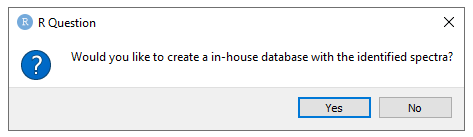
\includegraphics[width=0.4\linewidth]{22} 

}

\caption{In-house database creation.}\label{fig:unnamed-chunk-41}
\end{figure}

For this extra step, the user may provide more information than the
name, retention time and index and spectrum. A dataInfo.csv will be
created in the folder, if the user agree to add more information, where
information about molecule describers such as CAS, InChiKey, PubChem ID,
ChemSpider ID, retention index and more can be included.

\begin{figure}

{\centering 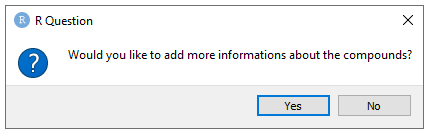
\includegraphics[width=0.4\linewidth]{23} 

}

\caption{Add more information to the compounds.}\label{fig:unnamed-chunk-42-1}
\end{figure}
\begin{figure}

{\centering 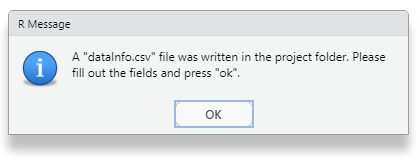
\includegraphics[width=0.4\linewidth]{24} 

}

\caption{Add more information to the compounds.}\label{fig:unnamed-chunk-42-2}
\end{figure}

After filling most of the information as possible, there can still be
missing information, as in the case of these example:

\begin{longtable}[]{@{}
  >{\raggedright\arraybackslash}p{(\columnwidth - 18\tabcolsep) * \real{0.1453}}
  >{\raggedright\arraybackslash}p{(\columnwidth - 18\tabcolsep) * \real{0.0769}}
  >{\raggedleft\arraybackslash}p{(\columnwidth - 18\tabcolsep) * \real{0.0940}}
  >{\raggedleft\arraybackslash}p{(\columnwidth - 18\tabcolsep) * \real{0.0769}}
  >{\raggedright\arraybackslash}p{(\columnwidth - 18\tabcolsep) * \real{0.1026}}
  >{\raggedright\arraybackslash}p{(\columnwidth - 18\tabcolsep) * \real{0.0940}}
  >{\raggedright\arraybackslash}p{(\columnwidth - 18\tabcolsep) * \real{0.2393}}
  >{\raggedleft\arraybackslash}p{(\columnwidth - 18\tabcolsep) * \real{0.0940}}
  >{\raggedright\arraybackslash}p{(\columnwidth - 18\tabcolsep) * \real{0.0513}}
  >{\raggedright\arraybackslash}p{(\columnwidth - 18\tabcolsep) * \real{0.0256}}@{}}
\toprule()
\begin{minipage}[b]{\linewidth}\raggedright
Name
\end{minipage} & \begin{minipage}[b]{\linewidth}\raggedright
formula
\end{minipage} & \begin{minipage}[b]{\linewidth}\raggedleft
exact.mass
\end{minipage} & \begin{minipage}[b]{\linewidth}\raggedleft
rt
\end{minipage} & \begin{minipage}[b]{\linewidth}\raggedright
CAS
\end{minipage} & \begin{minipage}[b]{\linewidth}\raggedright
ChemSpider
\end{minipage} & \begin{minipage}[b]{\linewidth}\raggedright
InChIKey
\end{minipage} & \begin{minipage}[b]{\linewidth}\raggedleft
PubChem.ID
\end{minipage} & \begin{minipage}[b]{\linewidth}\raggedright
Class
\end{minipage} & \begin{minipage}[b]{\linewidth}\raggedright
RI
\end{minipage} \\
\midrule()
\endhead
Palmitic acid & C16H32O2 & 256.2402 & 687.3255 & 408-35-5 & NA &
IPCSVZSSVZVIGE-UHFFFAOYSA-N & 985 & NA & NA \\
Inositol & C6H12O6 & 180.0634 & 645.7250 & 173524-45-3 & NA &
CDAISMWEOUEBRE-UHFFFAOYSA-N & 892 & NA & NA \\
Tyrosine & C9H11NO3 & 181.0739 & 650.3799 & 55520-40-6 & NA &
OUYCCCASQSFEME-QMMMGPOBSA-N & 6057 & NA & NA \\
Allantoin & C4H6N4O3 & 158.0440 & 632.7000 & 5377-33-3 & NA &
POJWUDADGALRAB-UHFFFAOYSA-N & 204 & NA & NA \\
FAME C16 & C17H34O2 & 270.5000 & 660.1515 & & NA &
FLIACVVOZYBSBS-UHFFFAOYSA-N & NA & NA & NA \\
p-Coummaric acid & C9H8O3 & 164.1600 & 676.7077 & & NA &
NGSWKAQJJWESNS-ZZXKWVIFSA-N & NA & NA & NA \\
\bottomrule()
\end{longtable}

After filling the forms and pressing `Ok', the software will still try
to recover the missing information and more. It will be asked if the
user would like to add retention index information, if there missing
indexes. For that, the user must provide the kind of retention index
(supported one are `linear', `lee' and `kovats') and from what
information to look for. It is recommended that the user provide a
InChiKey or CAS number for each compound for they are much more reliable
and non-ambiguous to look for in the NIST system in order to recover de
retention index information.If more than one retention index is present,
the the software returns the RI as a mean of the registered RIs.

\begin{figure}

{\centering 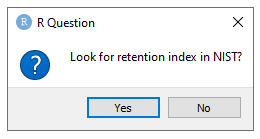
\includegraphics[width=0.4\linewidth]{25} 

}

\caption{Retention index information.}\label{fig:unnamed-chunk-44}
\end{figure}

Here we use InChiKey information and the user is asked to check the
DatabaseInfo.csv file and fill missing fields, if possible. The
resulting information file is as such:

\begin{longtable}[]{@{}
  >{\raggedright\arraybackslash}p{(\columnwidth - 18\tabcolsep) * \real{0.1382}}
  >{\raggedright\arraybackslash}p{(\columnwidth - 18\tabcolsep) * \real{0.0732}}
  >{\raggedleft\arraybackslash}p{(\columnwidth - 18\tabcolsep) * \real{0.0894}}
  >{\raggedleft\arraybackslash}p{(\columnwidth - 18\tabcolsep) * \real{0.0732}}
  >{\raggedright\arraybackslash}p{(\columnwidth - 18\tabcolsep) * \real{0.0976}}
  >{\raggedright\arraybackslash}p{(\columnwidth - 18\tabcolsep) * \real{0.0894}}
  >{\raggedright\arraybackslash}p{(\columnwidth - 18\tabcolsep) * \real{0.2276}}
  >{\raggedleft\arraybackslash}p{(\columnwidth - 18\tabcolsep) * \real{0.0894}}
  >{\raggedright\arraybackslash}p{(\columnwidth - 18\tabcolsep) * \real{0.0488}}
  >{\raggedleft\arraybackslash}p{(\columnwidth - 18\tabcolsep) * \real{0.0732}}@{}}
\toprule()
\begin{minipage}[b]{\linewidth}\raggedright
Name
\end{minipage} & \begin{minipage}[b]{\linewidth}\raggedright
formula
\end{minipage} & \begin{minipage}[b]{\linewidth}\raggedleft
exact.mass
\end{minipage} & \begin{minipage}[b]{\linewidth}\raggedleft
rt
\end{minipage} & \begin{minipage}[b]{\linewidth}\raggedright
CAS
\end{minipage} & \begin{minipage}[b]{\linewidth}\raggedright
ChemSpider
\end{minipage} & \begin{minipage}[b]{\linewidth}\raggedright
InChIKey
\end{minipage} & \begin{minipage}[b]{\linewidth}\raggedleft
PubChem.ID
\end{minipage} & \begin{minipage}[b]{\linewidth}\raggedright
Class
\end{minipage} & \begin{minipage}[b]{\linewidth}\raggedleft
RI
\end{minipage} \\
\midrule()
\endhead
Palmitic acid & C16H32O2 & 256.2402 & 687.3255 & 408-35-5 & NA &
IPCSVZSSVZVIGE-UHFFFAOYSA-N & 985 & NA & 1964.833 \\
Inositol & C6H12O6 & 180.0634 & 645.7250 & 173524-45-3 & NA &
CDAISMWEOUEBRE-UHFFFAOYSA-N & 892 & NA & NA \\
Tyrosine & C9H11NO3 & 181.0739 & 650.3799 & 55520-40-6 & NA &
OUYCCCASQSFEME-QMMMGPOBSA-N & 6057 & NA & NA \\
Allantoin & C4H6N4O3 & 158.0440 & 632.7000 & 5377-33-3 & NA &
POJWUDADGALRAB-UHFFFAOYSA-N & 204 & NA & NA \\
FAME C16 & C17H34O2 & 270.5000 & 660.1515 & NA & NA &
FLIACVVOZYBSBS-UHFFFAOYSA-N & NA & NA & 1917.444 \\
p-Coummaric acid & C9H8O3 & 164.1600 & 676.7077 & NA & NA &
NGSWKAQJJWESNS-ZZXKWVIFSA-N & NA & NA & NA \\
\bottomrule()
\end{longtable}

And the creation of the in-house database is concluded.

\begin{figure}

{\centering 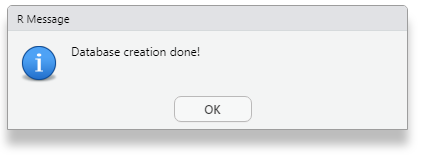
\includegraphics[width=0.4\linewidth]{28} 

}

\caption{In-house database created.}\label{fig:unnamed-chunk-46}
\end{figure}

\begin{center}\rule{0.5\linewidth}{0.5pt}\end{center}

\hypertarget{references}{%
\section{References}\label{references}}

\begin{enumerate}
\def\labelenumi{\arabic{enumi}.}
\item
  Abreu LGF, Silva N, Ferrari A, Carvalho L, Fiamenghi M, Carazolle M,
  Fill T, Pilau E, Pereira G, Grassi M: \textbf{Metabolite profiles of
  energy cane and sugarcane reveal different strategies during the
  axillary bud outgrowth}. \emph{Plant Physiology and Biochemistry},
  2021, \textbf{\emph{167}}:504-516.
\item
  NIST. \textbf{NIST Standard Reference Database 1A}. Available in:
  \url{https://chemdata.nist.gov/mass-spc/ms-search/docs/Ver20Man_11.pdf}.
\item
  TANAKA S, FUJITA Y, PARRY HE, YOSHIZAWA AC, MORIMOTO K, MURASE M,
  YAMADA Y, UTSUNOMIYA S, KAJIHARA K, FUKUDA M, IKAWA M, TABATA T,
  KATAHASHI K, AOSHIMA K, NIHEI Y, NISHIOKA T, ODA Y, TANAKA K:
  \textbf{Mass++: a visualization and analysis tool for mass
  spectrometry}. \emph{Journal Of Proteome Research}, 2014,
  \textbf{\emph{13}}:3846-3853.
\item
  KESSNER D, CHAMBERS M, BURKE R, AGUS D, MALLICK P:
  \textbf{ProteoWizard: open source software for rapid proteomics tools
  development}. \emph{Bioinformatics}, 2008,
  \textbf{\emph{24(21)}}:2534-6.
\end{enumerate}

\end{document}
